%%%%%%%%%%%%%%%%%%%%%%%%%%%%%%%%%%%%%
% This file is the "main" or root file for the book. It describes what packages
% and content should be included in what order.

\documentclass[14pt]{memoir}

\usepackage{comment}
\usepackage{etoolbox}
\usepackage{fancyvrb}
\usepackage{graphicx}
%\usepackage{hyperref}
\usepackage{xurl}
\usepackage[round]{natbib}
\usepackage{xspace}
\usepackage{amsmath}
\usepackage{algpseudocode}
\usepackage{algorithm}
%\usepackage{algorithmic}
\usepackage{multirow}
\usepackage{tikz}
\usepackage{boxedminipage}
\usepackage{alltt}
\usepackage{epigraph}
\usepackage{amssymb}
\usepackage{amsthm}
\usepackage[hashEnumerators,smartEllipses,hybrid]{markdown}
\def\sqrtofthree{1.732050808}
\usepackage{minted}

% This is for multilingual work. Would be nice to support Chinese and Thai.
\usepackage[utf8]{inputenc}                         % Acentuação direta
\usepackage[T1]{fontenc}  
\usepackage[portuguese]{babel}
\usepackage{listings}
\renewcommand{\lstlistingname}{Código} % Listing->Code
\usepackage{xcolor}



\definecolor{LightGray}{gray}{0.9}


\definecolor{lightblue}{rgb}{0.68, 0.85, 0.9}
\definecolor{mygreen}{rgb}{0,0.6,0}
\definecolor{mygray}{rgb}{0.5,0.5,0.5}
\definecolor{mymauve}{rgb}{0.58,0,0.82}

\lstset{ 
  backgroundcolor=\color{white},   % choose the background color; you must add \usepackage{color} or \usepackage{xcolor}; should come as last argument
  basicstyle=\footnotesize,        % the size of the fonts that are used for the code
  breakatwhitespace=false,         % sets if automatic breaks should only happen at whitespace
  breaklines=true,                 % sets automatic line breaking
  captionpos=b,                    % sets the caption-position to bottom
  commentstyle=\color{mygreen},    % comment style
  deletekeywords={...},            % if you want to delete keywords from the given language
  escapeinside={\%*}{*)},          % if you want to add LaTeX within your code
  extendedchars=true,              % lets you use non-ASCII characters; for 8-bits encodings only, does not work with UTF-8
  firstnumber=1,                % start line enumeration with line 1000
  frame=single,	                   % adds a frame around the code
  keepspaces=true,                 % keeps spaces in text, useful for keeping indentation of code (possibly needs columns=flexible)
  keywordstyle=\color{blue},       % keyword style
  morekeywords={*,...},            % if you want to add more keywords to the set
  numbers=left,                    % where to put the line-numbers; possible values are (none, left, right)
  numbersep=5pt,                   % how far the line-numbers are from the code
  numberstyle=\tiny\color{mygray}, % the style that is used for the line-numbers
  rulecolor=\color{black},         % if not set, the frame-color may be changed on line-breaks within not-black text (e.g. comments (green here))
  showspaces=false,                % show spaces everywhere adding particular underscores; it overrides 'showstringspaces'
  showstringspaces=false,          % underline spaces within strings only
  showtabs=false,                  % show tabs within strings adding particular underscores
  stepnumber=1,                    % the step between two line-numbers. If it's 1, each line will be numbered
  stringstyle=\color{mymauve},     % string literal style
  tabsize=2,	                   % sets default tabsize to 2 spaces
  title=\lstname                   % show the filename of files included with \lstinputlisting; also try caption instead of title
}

% This file is for commands / macros / functions.

% That at least was the original intention. As you can see from the comments, some of the commands
% that work for TeX and pdf output are innefective when applied to HTML and eBooks!

% These are useful because HTML output corrupts the result of the \latex command.
\newcommand{\latex}{LaTeX\xspace}
\newcommand{\tex}{TeX\xspace}
\newtheorem{exemplo}{Exemplo}[chapter]
\newtheorem{definition}{Definição}[chapter]
\newtheorem{theorem}{Teorema}[chapter]
\renewcommand\qedsymbol{$\blacksquare$}

% Makes extra space in HTML but not in PDF output.
\def\htbr{\ifdefined\HCode{\HCode{<br/><br/>}}\fi}

\newcommand\nextpage[1][]{
\ifdefined\HCode {
  \HCode{<mbp:pagebreak />}}
\else
  \newpage
\fi
}

% Makes small typewriter text, comparable to other font sizes.
\def\smalltt#1{\texttt{\small #1}}

% Makes small verbatim inline typewriter text, comparable to other font sizes.
% Use as \sverb|My verbatim text|
\def\sverb{\Verb[fontsize=\small]}

% Makes small URL text, comparable to other font sizes.
\def\surl#1{{\small{\url{#1}}}}


% This line stops the insertion of extra blank pages between chapters.
\ifdefined\HCode{\KOMAoptions{twoside=false}} \fi

\begin{document}

% Title and author are written down in the cover_page.tex file, and author
% appears also as an argument to the ebook-convert command in the build.sh file.
%% This is a cover page.

\thispagestyle{empty}

\vspace{3cm}
  \begin{center}
	\bfseries  \Huge Estrutura de Dados \par   % Your own title would go here.
        \bfseries \Large Wladimir Araújo Tavares \par   % The author's name goes here.
        \vspace{3cm}
      	{\centering 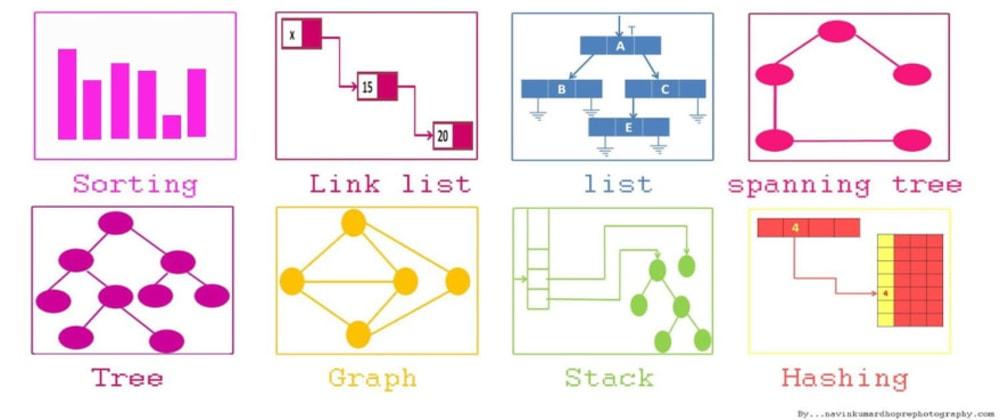
\includegraphics[width=1.0\linewidth,scale=1.5]{images/cover.jpg}}
    \end{center}
    
\par

\newpage


\tableofcontents

%\nextpage
%%%%
\chapter{Recursividade}

\section{Definições Recursivas de funções}

Em alguns casos, pode ser difícil definir um objeto explicitamente. Nestes casos, podemos definir um objeto em termos dele mesmo. Esse processo é chamado recursão.


Considere o seguinte exemplo: 

\begin{exemplo}
Uma linha de quadrados é construída usando palitos de fósforo, como mostrado na figura abaixo.


\begin{figure}[htbp]
\centering
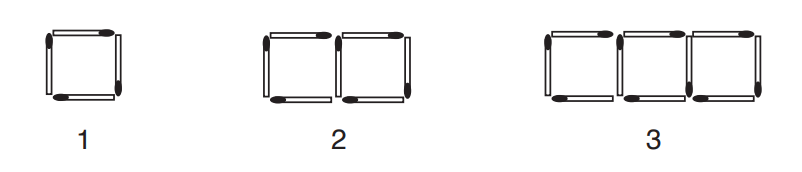
\includegraphics[width=.9\textwidth]{images/fosforos.png}
\label{fig:exampleFig2}
\end{figure}

Quantos palitos são necessários para a construção de uma linha de $n$ quadrados? 

Podemos definir uma função recursivamente para resolver este problema acima. A definição recursiva de uma função pode ser separada em dois casos:

\begin{itemize}
    \item Passo Base: Especifica o valor da função para o menor valor.
    \item Passo Recursivo: Apresenta uma regra para obter o valor para um número n a partir de casos menores.
\end{itemize}

Seja $f(n)$ o número de palitos necessários para construir uma linha de $n$ quadrados.

\begin{itemize}
    \item Passo Base: $f(1) = 4$
    \item Passo Recursivo: $f(n) = f(n-1) + 3$
\end{itemize}

Observe que juntando 3 novos palitos a linha de 1 quadrado podemos construir uma linha de 2 quadrados. No caso geral, se juntamos 3 novos palitos a uma linha de $n-1$ quadrados obtemos uma linha de $n$ quadrados.
\end{exemplo}

\newpage

\begin{exemplo}

João trabalha no supermercado, e seu gerente pediu que ele empilhasse latas de ervilhas como na figura abaixo.

\begin{center}
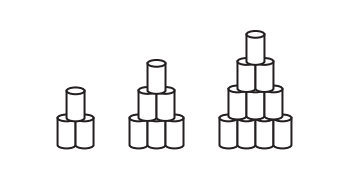
\includegraphics{images/Latas.png} 
\end{center}

Proponha uma definição recursiva para o número de latas necessárias para construir uma pilha de latas nesse formato com altura de $n$ latas. 

Seja $p(n)$ o número de latas necessárias para construir uma pilhas de latas no formato acima com uma altura $n$. Note que a pilha de altura 1 pode ser construída com apenas uma única lata.
Observe que podemos construir uma pilha de latas nesse formato com altura de $n$ latas, colocando $n$ latas na base e colocando a pilha de latas de altura $n-1$ sobre a base de $n$ latas. Dessa maneira, a definição recursiva para $p(n)$ será:

$$
p(n) = 
\begin{cases}
1 &  \text{ , $n$ =  1} \\
n + p(n-1) & \text{ , caso contrário}\\ 
\end{cases}
$$

\end{exemplo}





\begin{exemplo}
Imagine que você queira construir uma parede de tijolos com tijolos com o comprimento igual a duas vezes a sua altura. Considere que a nossa parede sempre terá apenas duas unidades de altura. Calcule de quantos padrões podemos construir uma parede com comprimento $n$.

\begin{figure}[!htbp]
\caption{Padrões de construções da parede com tijolos 1 x 2}
\label{fig::tijolos}
\begin{center}
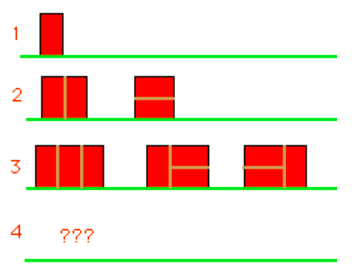
\includegraphics[scale=0.7]{images/pattern.png} 
\end{center}
\end{figure}

A Figura \ref{fig::tijolos} mostra a parede de comprimento igual a 3 pode ser construída de 3 maneiras diferentes.

Seja $t(n)$ o número de maneira de construir uma parede de comprimento $n$ com altura 2 usando apenas o tijolo 2x1. Note que podemos colocar o primeiro tijolo na parede de duas maneiras: um em pé ou dois tijolos deitados. Se colocarmos um tijolo em pé na parede de comprimento 3, podemos completar parede de duas maneiras diferentes ($t(2)$). Se o colocamos dois tijolos deitados, podemos completar a parede apenas de uma maneira ($t(1)$). O argumento acima está exemplificado na Figura \ref{fig::tijolos2}. De maneira geral,

$$t(n) = 
\begin{cases}
1 & n = 1\\
2 & n = 2\\
t(n-1) + t(n-2) & n \geq 3\\
\end{cases}
$$

\begin{figure}[!htbp]
\caption{Construção da parede usando o pensamento recursivo}
\label{fig::tijolos2}
\begin{center}
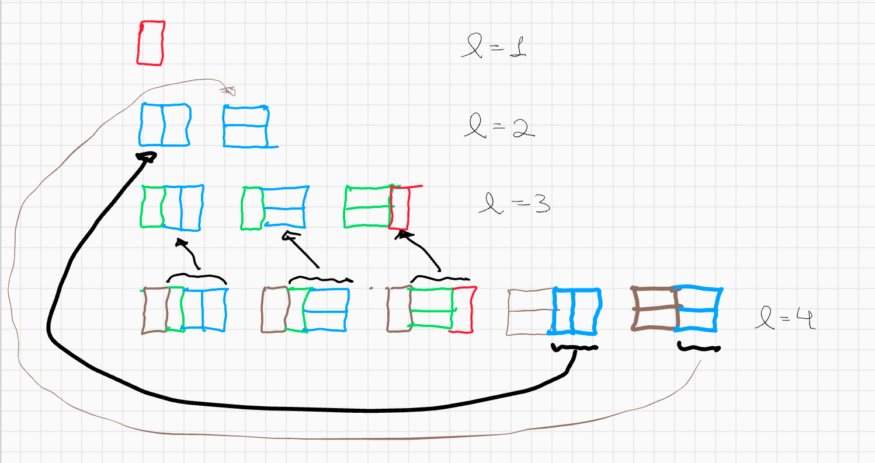
\includegraphics[scale=0.4]{images/tijolos.png} 
\end{center}
\end{figure}

\end{exemplo}



\begin{exemplo}
Você passa em uma loja perto de sua casa e vê a seguinte oferta: Uma garrafa de Choco Cola para cada 3 garrafas vazias devolvidas. Agora, você decide comprar algumas garrafas de cola nessa loja, quantas garrafas de cola você pode beber aproveitando essa promoção?

A Figura \ref{fig::chococola} mostra quantas garrafas de chococola você pode beber comprando inicialmente 8 garrafas de chococola.


\begin{figure}[!htbp]
\caption{Promoção chococola}
\label{fig::chococola}
\begin{center}
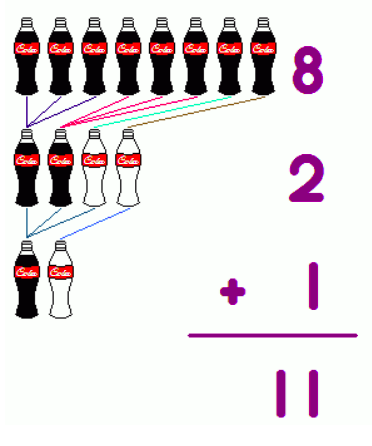
\includegraphics[scale=0.6]{images/cola.png} 
\end{center}
\end{figure}

Dê uma definição recursiva para a função $coca(n,m)$ que devolve o número de garrafas que você pode beber considerando que você tem $n$ garrafas cheias e $m$ garrafas vazias.



Primeiramente, vamos considerar os casos mais simples da função $coca(n,m)$:
$$coca(n,m) = 
\begin{cases}
0 & \text{, $m \leq 2 \wedge n = 0$}\\
n & \text{, $n \leq 2 \wedge m = 0$} 
\end{cases}
$$

Quando o número de garrafas vazias for menor ou igual a 2 e o número de garrafas cheias for zero não bebemos nenhuma garrafa. Quando o número de garrafas cheias for menor ou igual a 2 e o número de garrafas vazias for zero, bebemos apenas as garrafas cheias. 

Agora vamos considerar os casos mais complexos, vamos separar em dois casos:

$$coca(n,m) = 
\begin{cases}
coca(0, n+m) & \text{, $n \geq 0$}\\
coca(\lfloor m/3 \rfloor ,m \textbf{ mod } 3) & \text{, caso contrário} 
\end{cases}
$$

\end{exemplo}


\begin{exemplo}
3 objetos distintos podem ser organizados em sequência de seis maneiras diferentes.

\begin{center}
\begin{tabular}{c}
A,B,C\\
A,C,B\\
B,A,C\\
B,C,A\\
C,A,B\\
C,B,A\\
\end{tabular}
\end{center}

Dê uma definição recursiva para a função $f(n)$ que devolve o número de maneiras que podemos organizar n objetos distintos em sequência.

Seja f(n) o número de maneiras que podemos organizar n objetos distintos em uma sequência de tamanho $n$. O primeiro elemento de uma sequência pode ser escolhido de $n$ maneiras restando $n-1$ objetos para ser organizado em uma sequência de tamanho $n-1$. Logo,

$$
f(n) = 
\begin{cases}
1 & n = 1\\
n \cdot f(n-1) & \text{caso contrário}\\
\end{cases}
$$

\end{exemplo}

\begin{exemplo}



3 objetos distintos podem ser organizados em uma sequência de tamanho 2 de seis maneiras diferentes.

\begin{center}
\begin{tabular}{c}
A,B\\
A,C\\
B,A\\
B,C\\
C,A\\
C,B\\
\end{tabular}
\end{center}

Dê uma definição recursiva para a função $f(n, k)$ que devolve o número de maneiras que podemos organizar n objetos distintos em sequência de tamanho $k$ tal $k \leq n$.


Seja f(n,k) o número de maneiras que podemos organizar $n$ objetos distintos em uma sequência de tamanho $k$ tal que $k \leq n$. O primeiro elemento de uma sequência pode ser escolhido de $n$ maneiras restando $n-1$ objetos para ser organizado em uma sequência de tamanho $k-1$. Logo,

$$
f(n,k) = 
\begin{cases}
n & k = 1\\
n \cdot f(n-1,k-1) & \text{caso contrário}\\
\end{cases}
$$

\end{exemplo}

\begin{exemplo}{Números de triângulos em uma grade triangular}


\begin{minipage}{\textwidth}

Quantos triângulos em pé (tamanhos variados)
  podemos encontrar em uma grade de triângulos com
  altura $n$?
  
\begin{center}
    \begin{tikzpicture}
    \foreach \i in {0,1,2,3,4} {
      \draw (0 + 0.5*\i, \i * 0.5 * \sqrtofthree) -- (4 - 0.5*\i, \i * 0.5 * \sqrtofthree);
      \draw (0:\i) -- (60:\i);
      \draw[xshift=4cm] (180:\i) -- (120:\i);
    }
    \end{tikzpicture}
    \qquad
    \begin{tikzpicture}
    \fill[yellow!80] (0,0) -- (3,0) -- (1.5,3*0.5*\sqrtofthree);
    \fill[green!80] (1.5,0.5*\sqrtofthree) -- (3.5,0.5*\sqrtofthree) -- (2.5,3*0.5*\sqrtofthree);
    \foreach \i in {0,1,2,3,4} {
      \draw (0 + 0.5*\i, \i * 0.5 * \sqrtofthree) -- (4 - 0.5*\i, \i * 0.5 * \sqrtofthree);
      \draw (0:\i) -- (60:\i);
      \draw[xshift=4cm] (180:\i) -- (120:\i);
    }
    \end{tikzpicture}
  \end{center}

Destacamos dois triângulos de tamanhos variados encontrados em um triângulo de altura 4.

\end{minipage}


Seja $t(n)$ o número de triângulos em pé de tamanho variados que podemos encontrar em um grade triangulas com altura $n$.

Para uma grade de altura $n = 1$, temos $t(1) = 1$ triângulo

\begin{center}
    \begin{tikzpicture}
      \draw (0,0) -- (4,0) -- (2,4*0.5*\sqrtofthree) -- cycle;
    \end{tikzpicture}
  \end{center}
  
Para uma grade de altura $n = 2$, temos $t(2) = 4$ triângulo.

\begin{itemize}
  \item 2 com o vértice superior coincidindo com o vértice superior do maior triângulo.
  \item 2 outros triângulos com o vértice superior diferente do vértice superior do maior triângulo.
\end{itemize}

\begin{center}

\begin{tabular}{ll}

     \begin{tikzpicture}
      \foreach \i in {0,1,2} {
        \draw (0 + 1*\i, \i * 1 * \sqrtofthree) -- (4 - 1*\i, \i * 1 * \sqrtofthree);
        \draw (0:2*\i) -- (60:2*\i);
        \draw[xshift=4cm] (180:2*\i) -- (120:2*\i);
      }
      \draw[fill=blue!80] (1,\sqrtofthree) -- (3,\sqrtofthree) -- (2,2*\sqrtofthree) -- cycle;
      \draw[ultra thick, red!80] (0,0) -- (4,0) -- (2, 2*\sqrtofthree) -- cycle;
      \draw[ultra thick, red!80] (0,0) -- (4,0) -- (2, 2*\sqrtofthree) -- cycle;
    \end{tikzpicture}
&
         \begin{tikzpicture}
      \foreach \i in {0,1,2} {
        \draw (0 + 1*\i, \i * 1 * \sqrtofthree) -- (4 - 1*\i, \i * 1 * \sqrtofthree);
        \draw (0:2*\i) -- (60:2*\i);
        \draw[xshift=4cm] (180:2*\i) -- (120:2*\i);
      }
     
      \draw[fill=green!80] (0,0) -- (2,0) -- (1,\sqrtofthree) -- cycle;     
      \draw[fill=yellow!80] (2,0) -- (4,0) -- (3,\sqrtofthree) -- cycle;
      
    \end{tikzpicture}\\
\end{tabular}
  \end{center}

Podemos encontrar alguma padrão para $n=4$?

\begin{center}
    \begin{tikzpicture}
    
    
    
    
    \foreach \i in {0,1,2,3,4} {
      \draw (0 + 0.5*\i, \i * 0.5 * \sqrtofthree) -- (4 - 0.5*\i, \i * 0.5 * \sqrtofthree);
      \draw (0:\i) -- (60:\i);
      \draw[xshift=4cm] (180:\i) -- (120:\i);
    }
    \end{tikzpicture}
  \end{center}


Temos 4 triângulos têm o vértice superior coincidente com o vértice superior do triângulo maior

  \begin{center}
    \begin{tikzpicture}
      \fill[red!80]  (0,0) -- (4,0) -- (2, 2*\sqrtofthree) -- cycle;
      \fill[blue!80] (0.5,0.5 * \sqrtofthree) -- (3.5,0.5 * \sqrtofthree) -- (2, 4*0.5*\sqrtofthree) -- cycle;
      \fill[green!80] (1,\sqrtofthree) -- (3,\sqrtofthree) -- (2, 4*0.5*\sqrtofthree) -- cycle;
      \fill[yellow!80] (1.5,1.5*\sqrtofthree) -- (2.5,1.5*\sqrtofthree) -- (2, 4*0.5*\sqrtofthree) -- cycle;

      \foreach \i in {0,1,2,3,4} {
        \draw (0 + 0.5*\i, \i * 0.5 * \sqrtofthree) -- (4 - 0.5*\i, \i * 0.5 * \sqrtofthree);
      }
      \draw (0,0) -- (4,0) -- (2,4*0.5*\sqrtofthree) -- cycle;
    \end{tikzpicture}
  \end{center}
  
Os outros triângulos cujos vértices superiores não coincidem com o vértice superior do triângulo maior podem aparecer nesses dois triângulos amarelos internos (t(n-1)). Observe que somamos todos os triângulos que estão nos dois triângulos amarelos, os triângulos que estão dentro do triângulo vermelho (t(n-2)) serão contados duas vezes




\begin{center}
        \begin{tikzpicture}
          \foreach \i in {0,1,2,3,4} {
            \draw (0 + 0.5*\i, \i * 0.5 * \sqrtofthree) -- (4 - 0.5*\i, \i * 0.5 * \sqrtofthree);
            \draw (0:\i) -- (60:\i);
            \draw[xshift=4cm] (180:\i) -- (120:\i);
          }
          \draw[fill=yellow!80] (1,0) -- (4,0) -- (2.5, 3*0.5*\sqrtofthree) -- cycle;
          \draw[fill=yellow!80] (0,0) -- (3,0) -- (1.5, 3*0.5*\sqrtofthree) -- cycle;
          \draw[fill=red]  (1,0) -- (3,0) -- (2,   2*0.5*\sqrtofthree) -- cycle;
        \end{tikzpicture}
\end{center}

A definição recursiva de $t(n)$ é:
$$
t(n) =
\begin{cases}
1  & n = 1 \\
4  & n = 2 \\
n + 2 \cdot t(n-1) - t(n-2) & n \geq 3\\
\end{cases}
$$

\end{exemplo}


\begin{exemplo}

Ao subir a escada de seu prédio, José às vezes sobe dois degraus de uma vez e às vezes sobe um de cada
vez. Sabendo que a escada tem 3 degraus, de quantas maneiras diferentes José pode subir a escada? Você
consegue generalizar para o caso de uma escada com $n$ degraus?


Primeiramente, vamos pensar nos casos menores:

\begin{itemize}
    \item Uma escada de 1 degrau, podemos subir as escadas de 1 maneira (1).
    \item Uma escada de 2 degrau, podemos subir as escadas de 2 maneiras (1+1,2).
    \item Uma escada de 3 degraus, podemos subir as escadas de 3 maneiras (1+1+1,1+2,2+1).
\end{itemize}

Seja $x_n$ número de maneira de subir uma escada de $n$ degraus.  O primeiro passo para subir uma escada de n degraus pode ser dado de duas maneiras:

\begin{itemize}
    \item Se você subir apenas um degrau, então teremos $x_{n-1}$ maneiras de subir o restante da escada.
    \item Se você subir dois degraus, então teremos $x_{n-2}$ maneiras de subir o restante da escada.
\end{itemize}

A recorrência para $x_n$ será:

$$
x_n = \begin{cases}
1 & n = 1\\
2 & n = 2\\ 
x_{n-1} + x_{n-2} & n \geq 3\\
\end{cases}
$$
\end{exemplo}

\begin{exemplo}
Quantas são as sequências de n termos pertencentes a \{0,1\} , que possuem um número ímpar de termos iguais a 0?

Por exemplo,

Sequências de tamanho 1: 1 (0) 

Sequências de tamanho 2: 2 ( 01 e 10)

Encontre uma relação de recorrência que relaciona o número de termos dessa sequência.

Seja f(n) o número de sequências de $n$ termos 0 e 1 com uma quantidade ímpar de termos iguais a 0. O número de sequência de $n+1$ termos 0 e 1 com um número ímpar de termos iguais a 0 é igual a soma:
\begin{itemize}
    \item do número de sequências começadas por 1 seguido por uma sequência de $n$ termos com um número ímpar de zeros 
    \item com o número de sequências começadas por zero seguido por um sequência de $n$ termos com um número par de zeros.
\end{itemize}


Portanto,

\begin{equation}
    f(n+1) = f(n) + 2^n - f(n) = 2^n
\end{equation}

Logo,

\begin{equation}
    f(n)  = 2^{n-1}
\end{equation}

\end{exemplo}

\section{Exercícios}


\begin{enumerate}
\item 



Suponha que um par de coelhos recém-nascidos, um macho e uma fêmea, sejam colocados em um campo. Os coelhos podem acasalar com um mês de idade, de modo que no final do segundo mês uma fêmea pode produzir outro casal de coelhos. Suponha que nossos coelhos nunca morram e que a fêmea sempre produz um novo par (um macho, uma fêmea) a cada mês a partir do segundo mês.  

\begin{center}
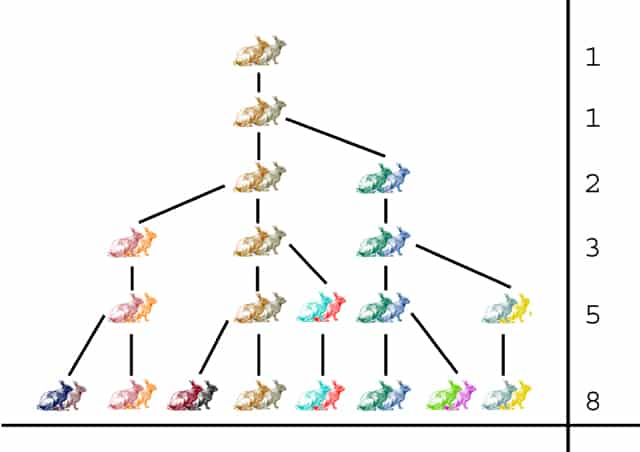
\includegraphics[scale=0.4]{images/rabbits.jpg} 
\end{center}

A imagem mostra que ao final do sexto mês teremos 8 pares de coelhos.


Quantos pares de coelhos teremos ao final de n meses?

Desenvolva uma função recursiva $f(n)$ que devolve o número de pares de coelhos após $n$ meses.

\item 




Suponha agora os nossos coelhos não vivam para sempre e morrem depois de k meses. Contudo, os coelhos acasalam com um mês de idade e cada fêmea produz um novo par de coelhos a cada mês a partir do segundo mês.


\begin{center}
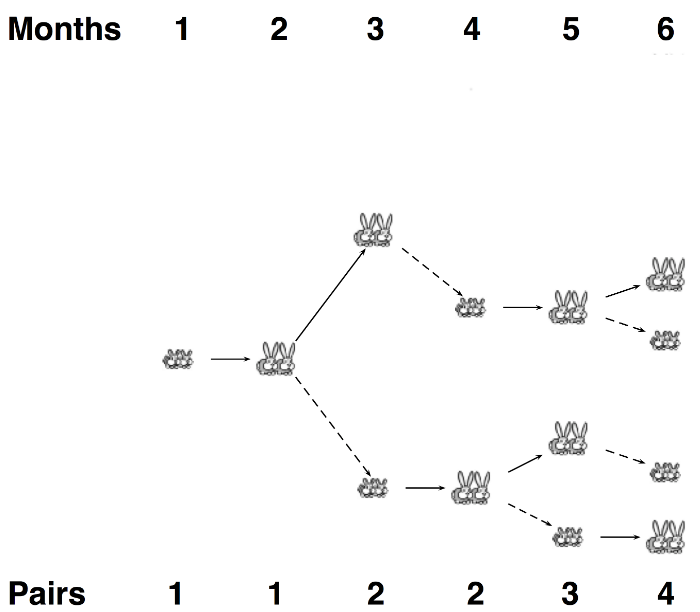
\includegraphics[scale=0.4]{images/rabbits2.png} 
\end{center}

A imagem mostra que ao final de seis meses teremos apenas 4 pares de coelhos considerando que os coelhos morrem após 3 meses.

Quantos pares de coelhos teremos ao final de n meses?

Desenvolva uma função recursiva $f(n,k)$ que devolve o número de pares de coelhos após $n$ meses considerando que os coelhos morrem depois de k meses. 



\item 

Ao subir a escada de seu prédio, José  sobe 1, 2 ou 3 degraus de uma vez. Sabendo que a escada tem 5 degraus, de quantas maneiras diferentes José pode subir a escada? Você
consegue generalizar para o caso de uma escada com $n$ degraus?

\item 

Quantas são as sequências de n termos pertencentes a \{0,1,2\} , que não possuem dois zeros consecutivos?

Por exemplo,

Sequências de tamanho 1: 3 (0,1 e 2) 

Sequências de tamanho 2: 8 ( 01,02,10,11,12,20,21 e 22)

\item 

Quantas são as sequências de n termos pertencentes a \{0,1,2\} , que não possuem dois zeros consecutivos?

Por exemplo,

Sequências de tamanho 1: 3 (0,1 e 2) 

Sequências de tamanho 2: 8 ( 01,02,10,11,12,20,21 e 22)

Faça um programa que gere todas as sequências de tamanho $n$ com termos pertencentes  a \{0,1,2\} , que não possuem dois zeros consecutivos.


\item 

Quantas são as sequências de n termos pertencentes a \{0,1,2\} , que possuem um número ímpar de termos iguais a 0?

Por exemplo,

Sequências de tamanho 1: 1 (0) 

Sequências de tamanho 2: 4 ( 01, 10, 20 e 02)

Encontre uma relação de recorrência que relaciona o número de termos dessa sequência.

\item 

Renata montou uma sequência de triângulos com palitos de fósforo, seguindo o padrão indicado na figura abaixo.

\begin{center}
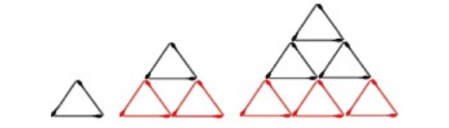
\includegraphics[width=1.0\linewidth,scale=0.8]{images/palitos.png} 
\end{center}

Quantos palitos serão usados por Renata no n-ésimo termo dessa sequência?

\item
Começando com um quadrado de 1cm de lado, formamos uma sequência de figuras, ob-
serve a figura abaixo. Cada figura, a partir da segunda, é formada unindo-se três cópias
da anterior. Os contornos destacados em vermelho das quatro primeiras figuras medem,
respectivamente, 4cm, 8cm, 20cm e 56cm. Quanto mede o contorno da figura n?


\begin{center}
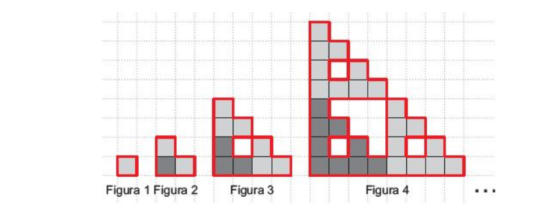
\includegraphics[width=1.0\linewidth,scale=0.8]{images/figura_recursiva.png} 
\end{center}

\item 

Um convidado em uma festa é uma celebridade se essa pessoa for conhecida por todos os outros convidados, mas não conhece nenhum deles. Existe no máximo uma celebridade em uma festa, pois se houvesse duas, eles se conheceriam.. Uma festa particular pode não ter celebridade. Sua tarefa é encontrar a celebridade, se ela
existe, em uma festa, fazendo apenas um tipo de pergunta - perguntando a um convidado se ele conhece um segundo convidado. Todos devem responder às suas perguntas com sinceridade. Ou seja, se Alice e Bob são duas pessoas na festa, você pode perguntar a Alice se ela conhece Bob; ela deve responder corretamente.

Seja $G(n)$ o número de perguntas utilizada para encontrar uma celebridade em uma festa com n pessoas.

\begin{enumerate}
    \item Calcule $G(1)$, $G(2)$, $G(3)$
    \item Proponha uma definição recursiva para $G(n)$. [Dica: primeiro faça uma pergunta para eliminar uma pessoa como celebridade. Em seguida, identifique  uma celebridade em potencial. Por fim, faça mais duas perguntas para determinar se a celebridade em potencial é na verdade uma celebridade.]
\end{enumerate}


\item 

Suponha que existem $n$ pessoas em um grupo, cada pessoa está ciente de um escândalo que
ninguém mais no grupo sabe sobre. Essas pessoas conversam por telefone; quando duas pessoas no grupo conversam, elas compartilham informações sobre todos os escândalos que cada um conhece. Para
por exemplo, na primeira chamada, duas pessoas compartilham informações, então
ao final da ligação, cada uma dessas pessoas sabe sobre dois escândalos. O problema da fofoca pede $G(n)$, o mínimo número de chamadas telefônicas necessárias para todas as n pessoas para
aprenda sobre todos os escândalos. 

\begin{enumerate}
    \item Mostre $G(1) = 0$
    \item Mostre $G(2) = 1$
    \item Mostre $G(3) = 3$
    \item Mostre $G(4) = 4$
    \item Mostre $G(5) = 6$
    \item Proponha um definição recursiva para $G(n)$
    
    
\end{enumerate}

\end{enumerate}













\section{Algoritmo Recursivo}

Um algoritmo é dito recursivo quando ele resolve um problema reduzindo para uma instância do mesmo problema com uma entrada menor.

\begin{exemplo}{Exponenciação}

Considere a seguinte definição recursiva da exponenciação:

\begin{equation}
a^n = 
\begin{cases}
1           & , n = 0\\
a * a^{n-1} & , n \geq 1
\end{cases}
\end{equation}
\end{exemplo}
O algoritmo recursivo para calcular $a^n$:

\begin{minted}{C++}
int exp(int a, int n){
	if(n==0) return 1;
	else return a*exp(a, n-1);
}
\end{minted}



No algoritmo acima, realizamos $n-1$ multiplicações para calcular $a^n$. Podemos fazer melhor utilizando uma outra definição recursiva.


\begin{exemplo}{Exponenciação rápida}

\begin{equation}
a^n = 
\begin{cases}
1           & , n = 0\\
(a^{n/2})^2 & , \text{$n$ é par}\\
a * a^{n-1} & , \text{$n$ é ímpar}

\end{cases}
\end{equation}
\end{exemplo}
\begin{minted}{C++}
int fast_exp(int a, int n){
    if(n==0) return 1;
    if(n%2==0){
        int res = fast_exp(a,n/2);
        return res*res;
    }else{
        return a*fast_exp(a, n-1);
    }
    
}
\end{minted}




\begin{exemplo}{soma de um vetor}

A definição recursiva da soma dos elementos de um vetor $a$ com índices variando entre $start$ e $end$:

\begin{equation}
soma(a, start, end) = 
\begin{cases}
a[start]           & , start = end\\
a[start] + soma(a, start+1, end) & , \text{caso contrário}\\

\end{cases}
\end{equation}


O algoritmo recursivo para calcular a soma dos elementos entre os duas posições start e end.

\begin{minted}{C++}
int soma_vetor(int *a, int start, int end){
	if( start == end ){
		return a[start];
	}else{
		return a[start] + soma_vetor(a, start + 1, end);
	}
}
\end{minted}

\end{exemplo}

\begin{exemplo}{Palavra palíndroma}

Considere a definição recursiva da função $is\_palindrome(s,i,j)$  que verificar se um palavra $s[i\ldots j]$ é palíndroma :

\begin{equation}
is\_palindrome(a, start, end) = 
\begin{cases}
true , start > end\\
true , start = end\\
s[start] == s[end] \&\& is\_palindrome(s, start+1, end-1)  \text{, caso contrário}\\

\end{cases}
\end{equation}




Observe que para testar se uma palavra com tamanho maior ou igual a 2, precisamos testar se o primeiro e o último caractere são iguais, depois precisamos testar se a palavra obtida pela remoção do primeiro e do último caractere  também é palíndroma.

\begin{minted}{C++}
bool is_palindrome(char s[], int i, int j){
    
    //palavra vazia
    if( i  > j ) return true;  
    //palavra de tamanho 1
    if( i == j ) return true; 
    
    if( s[i] == s[j] )
        return is_palindrome(s, i+1, j-1);
    else
        return false;
    
}
\end{minted}

\end{exemplo}


\begin{exemplo}{Busca linear}

Dado um vetor não-ordenado de inteiros de tamanho $n$ ( $a_0,a_1, \ldots, a_{n-1}$) e um um inteiro x. Implemente a função $busca(a, i, j, x)$ que devolve o índice da primeira ocorrência de x no subvetor $a_i, a_{i+1}, \ldots, a_j$, caso contrário, devolve -1. 

A função $busca(a, i, j, x)$ pode ser definida recursivamente da seguinte maneira:

\begin{equation}
busca(a, i, j , x) = 
\begin{cases}
  i, \text{se } A[i] = x\\
 -1, \text{se } i == j \\
busca(a, i+1, j, x) \text{, caso contrário}\\

\end{cases}
\end{equation}

\begin{minted}{C++}
int busca( int * A, int i, int j, int x){
    if( A[i] == x ) return i;
    else if(i == j) return -1;
    else return busca(A, i+1, j, x);
}
\end{minted}


\end{exemplo}

\begin{exemplo}
Dado um vetor de inteiros $arr$ de tamanho n existe uma posição k tal que 

$$arr[0] < arr[1] < ... < arr[k] > arr[k+1] > arr[k+2] > ... > arr[n-1]$$

Descubra $k$ usando a busca binária.

A função $pico(a, p, r)$ que devolve o valor de $k$ no intervalo $[p,r]$ pode ser definida recursivamente

\begin{equation}
pico(A, p, r) = 
\begin{cases}
  p  & \text{, se } p = r\\
  max(A[p],A[r]) & \text{, se } r == p+1 \\
  mid & \text{,} A[mid] > A[mid-1] \text{ e } A[mid] > A[mid+1]  \\
  pico(A, mid+1,r)      & \text{,} A[mid] < A[mid+1] \text{ e } A[mid-1] < A[mid]   \\
  pico(A, p,mid-1)      & \text{,} A[mid-1] > A[mid]    \\
\end{cases}
\nonumber 
\end{equation}
onde mid = (p+r)/2;


\begin{minted}{C++}
int pico(vector <int> & A, int p, int r){
    if( r-p == 0 ){ // tamanho 1
        return p;
    }else if( r-p == 1){ // tamanho 2 
        if(A[p] > A[r]) return p;
        else return r;
    }else{ // tamanho 3 ou mais
        int mid = p+r/2;
        if(A[mid] > A[mid-1] && A[mid] > A[mid+1]) return mid;
        if( A[mid-1] < A[mid]){
            if( A[mid] > A[mid+1] ) return mid;
            else{ // A[mid] < A[mid+1]
                return pico(A, mid+1, r);
            }
        }else{ // A[mid-1] > A[mid]  
            return pico(A, p, mid-1);
        }    
    }
}

\end{minted}
    
\end{exemplo}



\section{Exercícios}

\begin{enumerate}
    \item Proponha um algoritmo recursivo para encontrar o máximo de um vetor de tamanho $n$ usando o fato que o máximo de n inteiros é o maior entre o último inteiro do vetor e o máximo dos primeiros n-1 inteiros do vetor. 
    
    \item Proponha um algoritmo recursivo para computar o maior divisor comum de dois inteiros não negativos $a$ e $b$ com a  < b usando o fato que $mdc(a,b) = mdc(a, b-a)$. Note que se um número $d$ divide $a$ e $b$ então ele divide $a$ e $b-a$.
    
    \item Proponha um algoritmo recursivo para encontrar a primeira ocorrência de um valor x em um vetor ordenado de tamanho $n$ ( $a_0,a_1, \ldots, a_{n-1}$). Implemente a função $busca(a, i, j, x)$ que procura a primeira ocorrência de x no subvetor $a_i, a_{i+1}, \ldots, a_j$. 
    
    \item Proponha um algoritmo recursivo para multiplicar dois inteiros não-negativos baseado no fato que $x \cdot y = 2 \cdot (x \cdot y/2)$ quando $y$ é par e $x \cdot y = 2( x \cdot \lfloor y / 2 \rfloor) + x$ quando $y$ é ímpar, juntamente com a condição inicial que $x \cdot y = 0$ quando $y = 0$ 
    
    \item Proponha um algoritmo recursivo para computar $n^2$ para todo n inteiro não negativo usando o fato que $(n+1)^2 = n^2 + 2n + 1$.
    
    \item Seja $A = \{a^ib^i| i \in \mathbb{N}\}$ um conjunto de palavras. Proponha um algoritmo que recebe uma palavra $s$ de tamanho $n$ e verifica se $s \in A$. Dica: faça um função $check(s, 0, n-1)$ que verifica que se $s[0\ldots n-1]$ pertence ao conjunto  $A$.
    
    \item Seja $A = \{a^ib^ia^jb^j| i,j \in \mathbb{N}\}$ um conjunto de palavras. Proponha um algoritmo que recebe uma palavra $s$ de tamanho $n$ e verifica se $s \in A$. Dica: faça um função $check(s, 0, n-1)$ que verifica que se $s[0\ldots n-1]$ pertence ao conjunto  $A$.
    
    
    %\item Proponha um algoritmo recursivo que recebe dois vetores ordenados de tamanho $n$ e $m$ e devolve um vetor ordenado de tamanho $n+m$ com os elementos dois vetores dados. 
    
    \item Escreva uma função recursiva que calcule a soma dos dígitos decimais de um inteiro positivo.
Por exemplo, a soma dos dígitos de 132 é 6.

    \item O coeficiente binomial é uma relação estabelecida entre dois números naturais $n$ e $k$, $n\geq k\geq 0$, indicada por:

\begin{equation}
\binom{n}{k} = \frac{n!}{k!(n-k)!}  
\end{equation}   


Escreva uma função recursiva que calcule o coeficiente binomial de dois números inteiros não negativos $n$ e $k$, $n\geq k$.
 
Dica: Use a relação de Stifel:

\begin{equation}
\binom{n-1}{k-1} + \binom{n-1}{k} = \binom{n}{k}
\end{equation}



\item Uma sequência do gray code de n bits é uma sequência de $2^n$ inteiros onde:

\begin{itemize}
\item Cada número inteiro está no intervalo inclusivo [0, $2^n - 1$],
\item O primeiro inteiro é 0,
\item Um número inteiro aparece no máximo uma vez na sequência,
\item A representação binária de cada par de inteiros adjacentes difere em exatamente um bit, e
\item A representação binária do primeiro e do último inteiro difere exatamente um bit.
\end{itemize}

Dado um inteiro n, retorna qualquer sequência de gray code de n bits válida.

\begin{center}
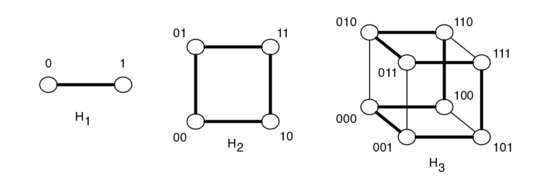
\includegraphics[scale=0.8]{images/hipercubo.png} 
\end{center}

\item Três marinheiros naufragaram em uma ilha e eles coletaram uma grande pilha de cocos durante o dia. Naquela noite, o primeiro marinheiro acorda e decide pegar sua primeira porção mais cedo, então tenta dividir a pilha de cocos igualmente em três pilhas, mas descobre que sobrou um coco, então ele o joga para um macaco e depois esconde sua parte das três pilhas de cocos do mesmo tamanho e junta as outras duas pilhas juntas para formar uma única pilha visível de cocos novamente e vai para a cama.

Para encurtar a história, cada um dos marinheiros, por sua vez, se levanta uma vez durante a noite e executa as mesmas ações de dividir a pilha de coco em três, descobrindo que sobrou um coco e dando aquele único coco restante ao macaco.

Pela manhã (após a ação clandestina e separada de cada um dos cinco marinheiros durante a noite), os cocos restantes são divididos em três pilhas iguais para cada um dos marinheiros, após o que se verifica que a pilha de cocos se divide igualmente entre os marinheiros sem resto. (Nada para o macaco pela manhã.)

Faça um programa que dado um inteiro N representando o número inicial de marinheiros encontre o número piha de cocos coletadas inicialmente. 

\textbf{Entrada}

Uma linha contendo um inteiro (N  $\leq$ 9 ) representando o número de marinheiro.

\textbf{Saída}

Devolva um inteiro representando o número de coco coletados inicialmente.\\

\textbf{Entrada}\\
3\\

\textbf{Saída} \\
25\\

\item \textbf{TapiocaSort} Preparar a pilha perfeita de tapiocas é uma tarefa complicada, porque não importa como você tenta todas as tapiocas em qualquer pilha têm diâmetros diferentes. Para o bem da limpeza, no entanto, você pode ordenar a pilha por tamanho de forma que cada tapioca seja menor do que todos os panquecas abaixo dela. O tamanho de uma panqueca é dado pelo seu diâmetro.

A ordenação de uma pilha é feita por uma sequência de "viradas" de tapiocas. Uma virada consiste em inserir uma espátula entre duas tapiocas em uma pilha e virando (invertendo) todas as panquecas em a espátula (invertendo a subpilha).

Uma virada é especificado dando a posição da tapioca na parte inferior da subpilha a ser virada em relação a toda a pilha. A panqueca de baixo tem a posição 1, enquanto a panqueca de cima em uma pilha de n panquecas tem posição n.

Uma pilha é especificada dando o diâmetro de cada tapioca na pilha na ordem em que aparecem as tapiocas. Por exemplo, considere uma pilha de tapiocas abaixo em que a tapioca 5 é a primeira tapioca do vetor:

topo -> 5 1 2 3 4 |

Fazendo a operação virada 1 (a espátula está representada por |), obtemos a seguinte pilha de tapiocas:

topo -> 4 3 2 1 | 5

Fazendo a operação virada 2, obtemos a seguinte pilha de tapiocas:

topo -> 1 2 3 4 5

Observe que a pilha de tapioca pode ser ordenada utilizando duas operações de virada.

\textbf{Entrada}

A primeira linha da entrada contém um inteiro N representando o número de tapiocas.

A segunda linha contém N inteiros positivos representando uma pilha de tapiocas. Cada tapioca terá um diâmetro entre 1 e 30.

\textbf{Saída}

Seu programa deve imprimir uma sequência de viradas que resulte na pilha de tapioca ordenada de maneira que a maior tapioca está na parte inferior e a menor tapioca na parte superior. A sequência de viradas deve terminar com 0, indicando que não são mais necessárias viradas.


\begin{tabular}{|l|l|}
\hline
Exemplo de Entrada & Exemplo de Saída\\
5                & 1 2 0\\      
5 1 2 3 4        &\\
\hline
\end{tabular}


\begin{tabular}{|l|l|}
\hline
Exemplo de Entrada & Exemplo de Saída\\
5                & 1 0\\      
5 4 3 2 1        &\\
\hline
\end{tabular}

\item  Pão a metro é um tipo de sanduíche gigante que é uma excelente opção de lanche para torneios de programação, embora a experiência já tenha mostrado que o oferecimento de sanduiches pode gerar reclamação dos competidores. Outro grande problema é que algumas pessoas são mais gulosas que outras e, dessa maneira, acabam pegando pedaços maiores que os pedaços dos outros. Para a final da OBI, a coordenação estava pensando em providenciar pão a metro para os competidores, porém tais problemas os fizeram recuar na idéia.

Embora a idéia tenha sido momentaneamente abandonada, uma idéia simples surgiu: cortar previamente o pão em fatias de tamanho iguais e distribuí-las entre as pessoas. O único problema com tal idéia é que se o número de pessoas for muito grande, fica impraticável ter apenas um pão. Por exemplo, se quisermos que 1.000 pessoas recebam 20 centímetros de sanduíche, seria necessário um sanduíche de 20.000 centímetros, ou 200 metros!

Alguém levantou a seguinte hipótese: se houvesse N pessoas e fossem encomendados K sanduíches de empresas diferentes, cada qual com uma determinada metragem (tamanho) $M_i$ ($1 \leq i \leq K$), seria possível retirar desses pães N fatias de mesmo tamanho, possivelmente sobrando partes nao utilizadas. A questão seria: qual o tamanho inteiro máximo que essas fatias poderão ter?

Por exemplo, se tivermos K = 4, com os tamanhos (em centímetros) M1 = 120, M2 = 89, M3 = 230 e M4 = 177 e N = 10, podemos retirar N fatias iguais de tamanho máximo 57, pois assim conseguimos 2 fatias no primeiro pão, 1 no segundo, 4 no terceiro e 3 no quarto, totalizando as 10 fatias necessárias. Se tentarmos cortar fatias de tamanho 58, só será possível obter 3 fatias do terceiro pão, totalizando 9 e, portanto, 57 é realmente o melhor que podemos obter. Note que não podemos usar duas ou mais fatias menores de diferentes pães para formarmos uma fatia do tamanho selecionado. (ficaria muito deselegante dar um lanche recortado às pessoas).

Tarefa

Escreva um programa que, dados os tamanhos de pão disponíveis (em centímetros) e a quantidade de pessoas a serem atendidas, retorne o tamanho inteiro máximo (em cent ímetros) da fatia que pode ser cortada de maneira a atender todas as pessoas.

Entrada

A entrada contém um único conjunto de testes, que deve ser lido do dispositivo de entrada padrão (normalmente o teclado). A primeira linha da entrada contém um inteiro N que indica a quantidade pessoas ($1 \leq N \leq 10.000$). A segunda linha contém um inteiro K ($1 \leq K \leq 10.000$) que é a quantidade de sanduíches disponível. Na terceira linha há K inteiros M ($1 \leq M \leq 10.000$) separados por um espaço em branco representando o tamanho de cada pão.

Saída Seu programa deve imprimir, na saída padrão, uma única linha, contendo o tamanho inteiro máximo da fatia que pode ser cortada.

Exemplos


\begin{tabular}{|l|l|}
\hline
Entrada & Saída\\
\hline
10                & 57\\      
4        &\\
120 89 230 77 & \\
\hline
\end{tabular}


    
\end{enumerate}




















\section{Backtracking}

O algoritmo de backtracking pode ser entendido como um refinamento de um algoritmo de força bruta. No algoritmo de backtracking, a solução para um problema computacional é construída de maneira incremental assim que uma condição do problema é violada, o algoritmo retrocede e tenta a próxima alternativa.

Vamos exemplificar o funcionamento de um algoritmo de backtracking na solução de um problema de satisfação. Um problema de satisfação pode ser definido por uma tripla $(X, D, C)$ onde:

\begin{itemize}
    \item $X = \{X_1, X_2, \ldots, X_n\}$ é um conjunto de variáveis.
    \item $D = \{D_1, D_2, \ldots, D_n\}$ é o conjunto dos respectivos domínios de cada variável.
    \item $C = \{C_1,C_2, \ldots,C_m\}$ é o conjunto de restrições do problema.
\end{itemize}


\begin{algorithm}
  \caption{Algoritmo de Backtracking}\label{AIPal}
  \begin{algorithmic}
    \Function{Backtracking}{$i,n$}
    
    \If{i = n+1}
        \State save\_solution(X)
    \Else 
        \For{$j \in D_i$}
            \If{$X[i] = j$ não viola nenhuma restrição}
            \State X[i] $\leftarrow$ j
            \State Backtracking(i+1, n)
            \EndIf
        \EndFor
    \EndIf
     
    \EndFunction
  \end{algorithmic}
\end{algorithm}

\subsection{Problema das n rainhas}

No problema das $n$ rainhas, temos n variáveis $(Q[1],Q[2], \ldots, Q[n])$. Cada variável $Q[i]$ guarda a posição da linha da i-ésima rainha. Em tabuleiro $n \times n$, $Q[i] \in \{1, 2, \ldots, n\}$. Neste problema, temos $n$ variáveis e seus domínios tem $n$ valores distintos.  As restrições para o problema são as seguintes:

\begin{enumerate}
    \item $\forall { 1 \leq  i < j \leq n} \quad Q[i] \neq Q[j] $
    \item $\forall { 1 \leq  i < j \leq n} \quad Q[i] + i \neq Q[j] + j$.
    \item $\forall { 1 \leq  i < j \leq n} \quad Q[i] - i \neq Q[j] - j$.
\end{enumerate}

A restrição (1) garante que não teremos duas rainhas distintas na mesma linha. A restrição (2) garante que não teremos duas rainhas na mesma diagonal secundária. A restrição (3) garante que não teremos duas rainhas na mesma diagonal principal. 

No algoritmo de backtracking, essas restrições são verificadas de maneira incremental considerando as fixações das variáveis já realizadas.

O Código abaixo escrito em C++ implementa o algoritmo de backtracking para o problema da n rainhas descrito acima.

\begin{minted}{C++}
void place_queen(vector <int> Q, int r, int n, int & cont){
    if(r == n+1){
        cont++;
    }else{
        for(int j = 1; j <= n; j++){
            bool legal = true;
            for(int i = 1; i <= r-1; i++){
                if( Q[i] == j || Q[i] == j+r-i || Q[i] == j-r+i){
                    legal = false;
                }
            }
            if(legal){
                Q[r] = j;
                place_queen(Q, r+1, n, cont);
            }
        }
    }
}

\end{minted}

\subsection{Problema da soma de subconjuntos}

Dado um conjunto $S$ com $n$ elementos encontre um subconjunto $S' \subseteq S$ tal que a soma dos elementos de $S'$ seja igual a um valor $K$.

Esse problema pode ser modelado da seguinte maneira. Teremos $n$ variáveis $(X[1], X[2], \ldots, X[n])$. Cada variável X[i] pode assumir dois valores \{true, false\}. Se X[i] é true, então $S[i] \in S'$. Caso contrário $S[i] \not \in S'$.

O nosso problema terá uma única restrição:

\begin{itemize}
    \item $\sum_{i=1}^{n} X[i]\cdot S[i] = K$
\end{itemize}

O Código abaixo escrito em C++ implementa o algoritmo de backtracking para o problema da soma de subconjunto.

\newpage 

\begin{minted}{C++}
void subsetsum(vector <int> & S,vector <bool> X, int K, int i, int n){
    if(i == n){
        bool flag = true;
        cout << "{";
        for(int j = 0; j < i; j++){
            if(X[j])
                cout << S[j] << " ";
        }
        cout << "}" << endl;
    }else{
        int prev = 0;
        for(int j = 0; j < i; j++){
            if(X[j])
                prev += S[j];
        }
        
        int next = 0;
        for(int j = i+1; j < n; j++){
            next += S[j];
        }

        
        if(prev + next >= K){            
            X[i] = false;
            subsetsum(S, X, K,  i+1, n);
        }
        
        if(prev + S[i] <=  K){
            X[i] = true;
            subsetsum(S, X, K, i+1, n);
        }
    }
}

int main(){
    
    vector <int> S( {2,3,4,1,7,8});
    vector <bool> X;
    X.resize(S.size());
    int K = 5;
    subsetsum(S, X, K, 0, S.size());
}

//Output:
//{4 1 }
//{2 3 }

\end{minted}

\subsection{Exercícios}

\begin{enumerate}
\item 

No quebra-cabeças Unruly, você recebe um tabuleiro $n \times n$. Cada quadrado do tabuleiro é colorido inicialmente com as cores branco, preto e cinza. O objetivo do jogo é pintar cada quadrado com a cor cinza com preto ou branco, de forma que:

\begin{itemize}
    \item não há três quadrados consecutivos, horizontalmente ou verticalmente, são da mesma cor
    \item cada linha e coluna contém o mesmo número de quadrados pretos e brancos. 
\end{itemize}

\begin{center}
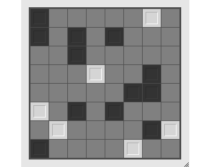
\includegraphics[scale=0.8]{images/unruly.png} 
\end{center}

Desenvolva um algoritmo de backtracking que resolva esse quebra-cabeça.

O jogo pode ser encontrado no seguinte link: \url{https://www.chiark.greenend.org.uk/~sgtatham/puzzles/js/unruly.html}

\item No quebra-cabeças Rectangles, você recebe uma grade retangular e alguns quadrados numerados.

\begin{center}
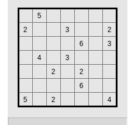
\includegraphics[scale=1.0]{images/Rectangles.png} 
\end{center}

Seu objetivo é traçar linhas paralelas as bordas grade rectangular para dividir a grade em retângulos, de modo que cada retângulo contenha exatamente um quadrado numerado e sua área seja igual ao número escrito naquele quadrado.

\begin{center}
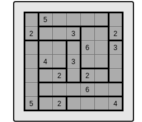
\includegraphics[scale=1.0]{images/Rectangles2.png} 
\end{center}

O jogo pode ser encontrado no seguinte link: \url{https://www.chiark.greenend.org.uk/~sgtatham/puzzles/js/rect.html}


\end{enumerate}






%\subsection{Maior subsequência crescente (Longest Increasing Subsequence)}

%Dado um vetor inteiro $A[1..n-1]$, nós precisamos encontrar a maior sequência de índices $i_1,i_2, \ldots, %i_l$ tal que $1 \leq i_1 < i_2 < \ldots < i_l \leq n$ e $A[i_1] < A[i_2] < \ldots < A[i_l]n$ 




% \section{Definição recursivas de conjuntos}

% Alguns conjuntos podem ser definidos de maneira recursiva. O conjuntos dos números pares positivos $P$ pode ser definido recursivamente da seguinte maneira:

% \begin{itemize}
%     \item $0 \in P$
%     \item Se $n \in P$ eentão $n+2 \in P$.
% \end{itemize}


% %Considere uma definição alternativa do conjuntos dos números pares positivos de maneira explicíta: 
% %\begin{equation}
% %P' = \{ 2k | k \in \mathbb{N} \}    
% %\end{equation}

% %É fácil mostrar que $P = P'$. 

% Seja S o conjunto dos pares ordenados de inteiros positivos $(a,b)$ tal que $2 | a + b$ pode ser definido recursivamente da seguinte maneira:

% \begin{itemize}
%     \item Passo Base: $(0,0) \in S$
%     \item Passo Recursivo Se $(a,b) \in S$ então $(a+1,b+1),(a+2,b),(a,b+2) \in S$.
% \end{itemize}

% O conjunto de todos os subconjuntos de um conjunto A, $subsets(A)$, pode ser definido recursivamente da seguinte maneira:

% \begin{itemize}
%     \item Passo Base: $\emptyset \in subsets(A)$
%     \item Passo Recursivo Seja $x \in A$, $Y \in subset(A\setminus \{x\})$ então $Y, Y \cup \{x\} \in subsets(A)$.
% \end{itemize}











 
%%%
\chapter{Análise de algoritmos}
\label{chapter:typesetting}


\epigraph{
“Um bom algoritmo, mesmo rodando em uma máquina lenta, sempre
acaba derrotando (para instâncias grandes do problema) um algoritmo
pior rodando em uma máquina rápida. Sempre.”

\textit{— S. S. Skiena, The Algorithm Design Manual}
}

\epigraph{

Um cientista americano perguntou para um cientista russo: Quando vocês desenvolveram a bomba atômica, como você conseguiram executar uma grande quantidade de cálculo com seus computadores fracos?. O cientista russo respondeu: "Nós desenvolvemos algoritmos melhores"
Anedota russa
}

Muitos fatores podem influenciar o tempo de execução de algoritmo. Inicialmente, precisamos de um modelo que seja genérico e independente da máquina/linguagem usada. 

No modelo Máquina de acesso aleatório (Random Access Machine  - RAM), consideramos as seguintes hipóteses:

\begin{itemize}
    \item As instruções são executadas uma após a outra, sem operações concorrentes.
    \item Cada operação simples (+,-,*,/,if) demora um 1 passo.
    \item Cada acesso à memória custa também um passo.
    \item As operações realizadas com dados inteiros e ponto flutuantes tem o mesmo custo.
\end{itemize}

Algumas implicações da adoção desse modelo:

\begin{itemize}
    \item A hierarquia de memória dos computadores é desprezada.
    \item A utilização de paralelismo também é desprezada.
\end{itemize}


\section{Analisando número de operações de um programa}

Considere o seguinte programa que dado um vetor de inteiros de tamanho $n$ conta o número de elementos iguais a zero.

\begin{lstlisting}[language=C, caption={primeiro programa}]
int count = 0;
for ( int i=0; i<n; i++)
    if (v[i] == 0) count++;
\end{lstlisting}

Contando o número de operações simples:

\begin{tabular}{|l|l|}
\hline
Operações & Número de operações\\
\hline
Declaração de variáveis & 2\\
\hline
Atribuições &  2\\
\hline
Comparação "menor que" & n+1\\
\hline
Comparação "igual a" & n\\
\hline
Acesso a um elemento do vetor & n\\
\hline
Incremento & entre n e 2n\\
\hline
\end{tabular}

Observe que o número de operações depende da instância de entrada do problema. O número de passos com relação ao tamanho da entrada será descrita pela função $T(n)$:


No pior caso, o número de operações será:

$$
T(n) = 2 + 2 + (n+1) + n+ n + 2n = 5n + 5
$$

No melhor caso, o número de operações será:

$$
T(n) = 2 + 2 + (n+1) + n+ n + n = 4n + 5
$$

Observe que o processo de análise de algoritmo, pode ser uma tarefa árdua se consideramos todas as operações simples envolvidas. Em geral, escolhemos a operação mais executada e contamos apenas quantas vezes ela está sendo executada. No exemplo acima, poderíamos ter analisado apenas o número de vezes que a operação de incremento está sendo executado.

Agora, iremos analisar o algoritmo de ordenação por inserção:

\begin{minted}{C++}
    int x, i; //2 declaracao
    // 1 declaracao, 1 atribuicao, n comparacoes, n incrementos 
    for(int j = 1; j < n; j++){ 
        x = A[j]; // n-1 atribuicao
        i = j-1; // n-1 atribuicao
        //n-1 vezes o while
        while(i >= 0 && A[i] > x){ // entre 1 e j comparações  
            A[i+1] = A[i]; //entre 0 e j-1 vezes atribuições
            i = i - 1;     // entre 0 e j-1 vezes decrementos
        }
        A[i+1] = x; // n-1 vezes atribuições
    }
\end{minted}

Diferente da análise anterior, vamos desprezar as seguintes operações básicas: 

\begin{itemize}
    \item declarações de variáveis
    \item Atribuições
    \item Acesso a um elemento de vetor
    \item incremento
\end{itemize}

Vamos contar apenas, o número de vezes que a operação $A[i] > x$ é realizada. 

No melhor caso, a operação $A[i] > x$ é realizada. 

$$
T(n) = \sum_{j=1}^{n-1} 1 = n-1 
$$

No pior caso, a operação $A[i] > x$ é realizada. 

$$
T(n) = \sum_{j=1}^{n-1} j = \frac{(1 + n-1)(n-1)}{2} = \frac{n(n-1)}{2} = \frac{n^2-n}{2} 
$$

Na próxima seção, apresentaremos uma ferramenta que possibilita a comparação entre algoritmos ou até mesmo a comparação entre o melhor caso e o pior caso de um mesmo algoritmo. Essa ferramenta é interessante porque podemos descobrir o comportamento do algoritmo para entradas grandes. No caso do algoritmo acima, para $n=2$, os dois algoritmos realizam o mesmo número de operações mas a situação muda dramaticamente a medida que o $n$ cresce.







\section{Análise Assintótica}

Considere dois algoritmos: $A_1$ que executa $n^2 + 1$ passos e $A_2$ que executa $n + 1000$ passos. A tendência da maioria das pessoas é considerar valores pequenos. Contudo, a análise de algoritmos faz exatamente o contrário: ignora os valores pequenos e concentra-se em valores grandes de $n$. Para isso, utilizaremos o comportamento assintótico. No caso acima, considere que $f(n) = n^2 +1$ e $g(n) = n + 1000$. Vamos mostrar que $f(n)$ domina assintoticamente $g(n)$ encontrando uma constante positivas  $c$ e $m$ tal que 

$$
g(n) \leq c f(n) \quad \forall n \geq m
$$


Considerando $f(n) = n^2 + 1$ e $g(n) = n + 1000$. Vamos fazer algumas manipulações algébricas para encontrar $c$ e $m$.

\begin{tabular}{ccc}
$n + 1000$     & $\leq$ &$n + 999 + 1$ \\
             & $\leq$ & $n^2 + 999n + 1$\\
             & $\leq$ & $n^2 + n^2 + 1 (n \geq 999)$\\
             & $\leq$ & $2n^2 + 1$ \\
             & $\leq$ & $2n^2 + 2$ \\
             & $\leq$ & $2(n^2 + 1)$ \\
             & $\leq$ & $2f(n))$ \\
\end{tabular}

Pelas manipulações acima, encontramos que $c = 2$ e $m = 999$

$$n + 1000 \leq 2( n^2 + 1 ) \quad \forall n \geq 999$$

Podemos encontrar outras constantes realizando manipulações algébricas diferentes.


\begin{tabular}{cccc}
$n + 1000$     & $\leq$ & $n^2$ & $(n \geq 33)$  \\
               & $\leq$ & $n^2 + 1$  \\
               & $\leq$ & $f(n))$   \\
\end{tabular}

Dado uma função $g(n)$, podemos encontrar um conjunto de funções que são dominadas assintoticamente por $g(n)$:

$$
\mathcal{O}(g(n)) = \{f(n) ~|~ \exists c, m, 0 \leq f(n) \leq c \cdot g(n) ~~ \forall n \geq m\}
$$

Em geral, escolhemos algumas funções para descrever o comportamento dos algoritmos:

\begin{itemize}
    \item $\mathcal{O}(1)$ (algoritmo constante)
    \item $\mathcal{O}(log ~n)$(algoritmo logarítmico)
    \item $\mathcal{O}(n)$ (algoritmo linear)
    \item $\mathcal{O}(n ~log ~n)$ (algoritmo linearítmico)
    \item $\mathcal{O}(n^2)$ (algoritmo quadrático)
    \item $\mathcal{O}(n^3)$ (algoritmo cúbico)
    \item $\mathcal{O}(2^n)$ (algoritmo exponencial)
    \item $\mathcal{O}(n!)$ (algoritmo fatorial)
    
    
    
\end{itemize}

\subsection{Comparações entre as classes de funções}

\small 

\begin{table}[!ht]
\begin{tabular}{ccccccc}
Tamanho & \multicolumn{6}{c}{Função de custo}                             \\
\hline
n       & $log_2n$ & $n$    & $nlog_2n$ & $n^2$   & $n^3$   & $2^n$       \\
\hline
10      & 3        & 10     & 30        & 100     & 1000    & 1000        \\
100     & 6        & $10^2$ & 664       & $10^4$  & $10^6$  & $10^30$     \\
$10^3$  & 9        & $10^3$ & 9965      & $10^6$  & $10^9$  & $10^300$    \\
$10^4$  & 13       & $10^4$ & $10^5$    & $10^8$  & $10^12$ & $10^3000$   \\
$10^5$  & 16       & $10^5$ & $10^6$    & $10^10$ & $10^15$ & $10^30000$  \\
$10^6$  & 19       & $10^6$ & $10^7$    & $10^12$ & $10^18$ & $10^300000$
\end{tabular}
\end{table}


\begin{itemize}
\item 1 semana $\approx$ $1,21\cdot 10^6$ segundos\\
\item 1 ano $\approx$ $3\cdot 10^7$ segundos\\
\item 1 século $\approx$ $3\cdot 10^9$ segundos\\
\item 1 milênio $\approx$ $3\cdot 10^{10}$ segundos\\
\end{itemize}


\begin{itemize}
  \item $O(n)$: linear
  \begin{itemize}
    \item quando $n$ dobra, o tempo dobra
    \item Ex: Busca linear
    \item Ex: Encontrar o máximo/mínimo de um vetor
    \item Ex: Produto interno de dois vetores
  \end{itemize}\medskip
  \item $O(n \lg n)$:
  \begin{itemize}
    \item quando $n$ dobra, o tempo um pouco mais que dobra
    \item Ex: algoritmos de ordenação que veremos
  \end{itemize}\medskip
  \item $O(n^2)$: quadrático
  \begin{itemize}
    \item quando $n$ dobra, o tempo quadriplica
    \item Ex: BubbleSort, SelectionSort e InsertionSort
  \end{itemize}\medskip
  \item $O(n^3)$: cúbico
  \begin{itemize}
    \item quando $n$ dobra, o tempo octuplica
    \item Ex: multiplicação de matrizes $n \times n$
  \end{itemize}
  
  \item $f(n) = O(c^n)$: complexidade exponencial
  \begin{itemize}
  \itemsep1em
  \item Típico de algoritmos que fazem busca exaustiva (força bruta) para resolver um problema.
  \item Não são úteis do ponto de vista prático.
  \begin{itemize}
   \item Quando $n$ é 20, $O(2^n)$ é um milhão.
  \end{itemize}
  \end{itemize}
  
  
  \item $f(n) = O(n!)$: complexidade exponencial
  \begin{itemize}
  \itemsep1em
  \item Pior que $O(c^n)$
  \item Não são úteis do pronto de vista prático.
  \item Quando $n$ é 20, $O(n!)$ é maior que 2 quintilhões.
  \end{itemize}
  
\end{itemize}


\subsection{Exercícios}

\textbf{Exercício:} Mostre que $2n+ 120 \in \mathcal{O}(n)$

\begin{proof}
Precisamos encontrar duas constantes $c$ e $m$, tal que

$$
2n + 120 \leq cn ~~\forall n \geq m
$$

Podemos encontrar essas constantes realizando algumas manipulações algébricas:

\begin{tabular}{llll}
2n + 120 & $\leq$ &  $2n + n$ & $(n \geq 120)$\\
         & $\leq$ &  $3n$ & \\ 
\end{tabular}

Encontramos os seguintes valores $c = 3$ e $m = 120$

Outros valores para c e m podem ser encontrados realizando diferentes manipulações algébricas:


\begin{tabular}{llll}
$2n + 120$ & $\leq$ &  $2n + 2n$ & $(n \geq 60)$\\
         & $\leq$ &  $4n$ & $(n \geq 60)$\\ 
\end{tabular}

Neste caso, encontramos $c=4$ e $m = 60$

\end{proof}


\textbf{Exercício:} Mostre que $3n^2+ n + 5 \in \mathcal{O}(n^2)$


\begin{proof}
Precisamos encontrar duas constantes $c$ e $m$, tal que

$$
3n^2 + n + 5 \leq cn^2 ~~\forall n \geq m
$$

Podemos encontrar essas constantes realizando algumas manipulações algébricas:

\begin{tabular}{llll}
$3n^2 + n + 5$ & $\leq$ &  $3n^2 + n^2 + n^2$ & $(n \geq 3)$\\
               & $\leq$ &  $5n^2$ & $(n \geq 3)$\\ 
\end{tabular}

Encontramos os seguintes valores $c = 5$ e $m = 3$


\end{proof}


\textbf{Exercício:} Mostre que $n^2  \not \in \mathcal{O}(n)$


\begin{proof}

Suponha por absurdo que  $n^2 \in \mathcal{O}(n)$

Então existem constantes $c$ e $m$ tal que
$$
n^2 \leq cn ~~\forall n \geq m
$$

Escolha $k = max(c, m) + 1$. Pela propriedade acima, $k^2 \leq kc$ $(k \geq m)$, segue o fato que $k \leq c$.

Pela construção de $k$, sabemos que $k > c$, o que é uma contradição. 

\end{proof}



\textbf{Exercício:} Mostre que $n ~log~ n  \not \in \mathcal{O}(n)$


\begin{proof}

Suponha por absurdo que  $n ~log n~ \in \mathcal{O}(n)$

Então existem constantes $c$ e $m$ tal que
$$
n~log~n \leq cn ~~\forall n \geq m
$$

Escolha $k = max(m, 2^c) + 1$. Pela propriedade acima, $k ~log k~ \leq ck$ $(k \geq m)$, segue o fato que $log k \leq c$.

Pela construção de $k$, sabemos que $k > 2^c$, logo $log k > c$ o que é uma contradição. 

\end{proof}


\section{Regras práticas}

\begin{itemize}
    \item $\forall f, f(n) \in \mathcal{O}(f(n))$
    \item Se $g(n) \in \mathcal{O}(f(n))$ então $c \cdot g(n) \in \mathcal{O}(f(n)) ~\forall c \in \mathbb{N}$
    \item Se $g(n) = a_kn^k + a_{k-1}x^{k-1} + \ldots + a_1n+ a_0 \in \mathcal{O}(f(n))$ então $g(n) \in \mathcal{O}(n^k)$
    \item Se $g(n) \in \mathcal{O}(f(n))$ e $h(n) =  g(n) + f(n)$ então $h(n) \in \mathcal{O}(f(n))$
\end{itemize}


\section{Analisando programas recursivos}

Considere o seguinte programa:


\begin{minted}{C++}
int piso_log2(int n){
    if(n <= 1) return 0;
    else return 1 + piso_log2(n/2);
}
\end{minted}

Vamos contar o número de vezes que a operação soma é realizada. Observe que o número de vezes que essa operação é realizada pode ser descrita utilizando a seguinte recorrência:

$$
T(n) = 
\begin{cases}
0 & n \leq 1\\
T( \lfloor n/2 \rfloor ) + 1 & \text{caso contrário}\\
\end{cases}
$$

Vamos tentar encontrar uma fórmula fechada utilizando o método da iteração. Primeiramente, vamos assumir que $n$ é uma potência de 2, $n = 2^k$. Faremos essa suposição para facilitar nosso cálculos.

\begin{tabular}{lll}
$T(2^k)$ & = & $T(2^{k-1}) + 1$ \\
       & = & $T(2^{k-2}) + 1 + 1$\\
       & = & $T(2^{k-3}) + 1 + 1 + 1$\\
       & = & $\ldots$ \\
       & = &  $T(2^{k-j}) + j$\\
\end{tabular}

Fazendo $j = k$, teremos

$$T(2^k) = T(2^0) + k = T(1) + k = 0 + k = k$$

Como $n = 2^k$, segue que $k = log_2 ~n$. Logo,

$$T(n) = log_2 n$$

Logo, podemos dizer que o algoritmo para encontrar o $\lfloor log_2(n) \rfloor$ realiza $O(log_2(n) )$ operações.

\subsection{Apêndice}

\begin{definition}
A notação de somatório é utilizada para expressar a soma dos termos de uma sequência $a_m, a_{m+1}, \ldots, a_n$. Nós usamos

$$
\sum_{j = m}^{n} a_j
$$

para representar

$$
a_{m} + a_{m+1} + \ldots + a_{n}
$$

A variável $j$ é chamada índice do somatório, $m$ é limite inferior do somatório e $n$ é o limite superior do somatório.

\end{definition}

\begin{theorem}
Para todo $n \in \mathbb{N}$,

$$\sum_{i=1}^{n} i = \frac{n(n+1)}{2}$$

\end{theorem}

\begin{proof}

Seja $S$ o soma dos números entre 1 e n. Na segunda linha, escrevemos o somatório na ordem contrária. Podemos agrupar o lado direto das equações como $n$ parcelas valendo $n+1$.

\begin{center}
\begin{tabular}{ccc}
     S & = & $1 + 2 + \ldots + n$   (1)\\
     S & = & $n + n-1 + \ldots + 1$ (2)\\ 
\hline
     S & = & $n+1 + n+1 + \ldots + n+1$ \\ 
    2S & = & $n(n+1)$\\
    S & = &  $\dfrac{n(n+1)}{2}$\\
\end{tabular}
    
\end{center}

A demonstração acima pode ser feita usando a notação de somatório:

$$
\begin{tabular}{ccc}
S  & = & $\displaystyle \sum_{i=1}^{n} i$\\
S  & = & $\displaystyle \sum_{i=1}^{n} n-i+1$\\
\hline
2S  & = & $\displaystyle \sum_{i=1}^{n} i+n-i+1$\\
2S  & = & $\displaystyle \sum_{i=1}^{n} n+1$\\
2S  & = & $\displaystyle n(n+1)$\\
S  & = & $\displaystyle \dfrac{n(n+1)}{2}$\\
\end{tabular}
$$
 
\end{proof}
\begin{definition}
Na lógica matemática, uma prova por contradição estabelece a verdade de uma proposição matemática assumindo que a proposição seja falsa obtendo uma contradição.
\end{definition}

\begin{theorem}
Seja $a,b \in \mathbb{N}$, $\forall n \geq 8$,  se $3a + 5b = n$ então $a \geq 2 \vee b \geq 1$.

Suponha por contradição que existe $n \geq 8$ tal que $3a + 5b = n \wedge \neg (a \geq 2 \vee b \geq 1)$. Suponha que $a < 1$ e $b < 0$ então  

$$
\begin{tabular}{ccc}
    a & $\leq$ & 1 \\
    b & $\leq$ & 0 \\
    3a & $\leq$ & 3 \\
    5b & $\leq$ & 0 \\
    3a + 5b & $\leq$ & 3 \\
\end{tabular}
$$

Por outro lado, sabemos $3a+5b \geq 8$, o que leva a uma contradição.
\end{theorem}





\chapter{Linguagem C++}

Bjarne Stroustrup começou a trabalhar em uma extensão da linguagem C, chamada C com classes, em 1979. Em 1985, Stroustrup lançou a primeira edição do livro "The C++ Programming Language". Este livro tornou-se a primeira documentação da linguagem. Até o momento, a linguagem possui seis revisões da padronização da linguagem:

\begin{center}
\begin{tabular}{ll}
Ano & Nome Informal\\
\hline
1998	&	C++98\\
2003	&	C++03\\
2011	&	C++11, C++0x\\
2014	&	C++14, C++1y\\
2017	&	C++17, C++1z\\
2020	&	C++20, C++2a\\
\end{tabular}
\end{center}

A linguagem C++ permite que você utilize diferentes paradigmas de programação como: procedural, orientado a objetos, funcional e genérica. Nessa disciplina, vamos utilizar de maneira extensiva os conceitos da programação orientada a objetos e programação genérica com a utilização dos templates da linguagem C++.













%%%
\chapter{Recursividade}

\section{Definições Recursivas de funções}

Em alguns casos, pode ser difícil definir um objeto explicitamente. Nestes casos, podemos definir um objeto em termos dele mesmo. Esse processo é chamado recursão.


Considere o seguinte exemplo: 

\begin{exemplo}
Uma linha de quadrados é construída usando palitos de fósforo, como mostrado na figura abaixo.


\begin{figure}[htbp]
\centering
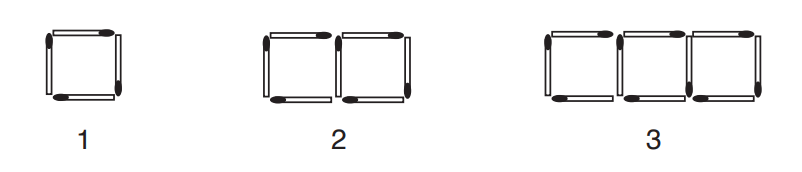
\includegraphics[width=.9\textwidth]{images/fosforos.png}
\label{fig:exampleFig2}
\end{figure}

Quantos palitos são necessários para a construção de uma linha de $n$ quadrados? 

Podemos definir uma função recursivamente para resolver este problema acima. A definição recursiva de uma função pode ser separada em dois casos:

\begin{itemize}
    \item Passo Base: Especifica o valor da função para o menor valor.
    \item Passo Recursivo: Apresenta uma regra para obter o valor para um número n a partir de casos menores.
\end{itemize}

Seja $f(n)$ o número de palitos necessários para construir uma linha de $n$ quadrados.

\begin{itemize}
    \item Passo Base: $f(1) = 4$
    \item Passo Recursivo: $f(n) = f(n-1) + 3$
\end{itemize}

Observe que juntando 3 novos palitos a linha de 1 quadrado podemos construir uma linha de 2 quadrados. No caso geral, se juntamos 3 novos palitos a uma linha de $n-1$ quadrados obtemos uma linha de $n$ quadrados.
\end{exemplo}

\newpage

\begin{exemplo}

João trabalha no supermercado, e seu gerente pediu que ele empilhasse latas de ervilhas como na figura abaixo.

\begin{center}
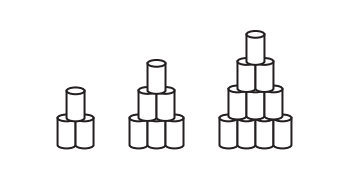
\includegraphics{images/Latas.png} 
\end{center}

Proponha uma definição recursiva para o número de latas necessárias para construir uma pilha de latas nesse formato com altura de $n$ latas. 

Seja $p(n)$ o número de latas necessárias para construir uma pilhas de latas no formato acima com uma altura $n$. Note que a pilha de altura 1 pode ser construída com apenas uma única lata.
Observe que podemos construir uma pilha de latas nesse formato com altura de $n$ latas, colocando $n$ latas na base e colocando a pilha de latas de altura $n-1$ sobre a base de $n$ latas. Dessa maneira, a definição recursiva para $p(n)$ será:

$$
p(n) = 
\begin{cases}
1 &  \text{ , $n$ =  1} \\
n + p(n-1) & \text{ , caso contrário}\\ 
\end{cases}
$$

\end{exemplo}





\begin{exemplo}
Imagine que você queira construir uma parede de tijolos com tijolos com o comprimento igual a duas vezes a sua altura. Considere que a nossa parede sempre terá apenas duas unidades de altura. Calcule de quantos padrões podemos construir uma parede com comprimento $n$.

\begin{figure}[!htbp]
\caption{Padrões de construções da parede com tijolos 1 x 2}
\label{fig::tijolos}
\begin{center}
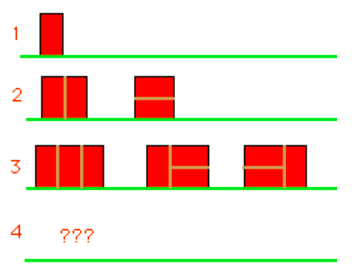
\includegraphics[scale=0.7]{images/pattern.png} 
\end{center}
\end{figure}

A Figura \ref{fig::tijolos} mostra a parede de comprimento igual a 3 pode ser construída de 3 maneiras diferentes.

Seja $t(n)$ o número de maneira de construir uma parede de comprimento $n$ com altura 2 usando apenas o tijolo 2x1. Note que podemos colocar o primeiro tijolo na parede de duas maneiras: um em pé ou dois tijolos deitados. Se colocarmos um tijolo em pé na parede de comprimento 3, podemos completar parede de duas maneiras diferentes ($t(2)$). Se o colocamos dois tijolos deitados, podemos completar a parede apenas de uma maneira ($t(1)$). O argumento acima está exemplificado na Figura \ref{fig::tijolos2}. De maneira geral,

$$t(n) = 
\begin{cases}
1 & n = 1\\
2 & n = 2\\
t(n-1) + t(n-2) & n \geq 3\\
\end{cases}
$$

\begin{figure}[!htbp]
\caption{Construção da parede usando o pensamento recursivo}
\label{fig::tijolos2}
\begin{center}
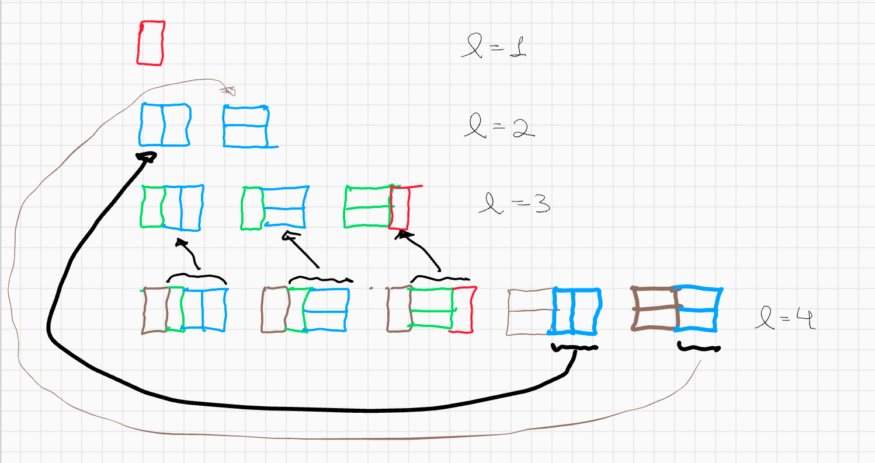
\includegraphics[scale=0.4]{images/tijolos.png} 
\end{center}
\end{figure}

\end{exemplo}



\begin{exemplo}
Você passa em uma loja perto de sua casa e vê a seguinte oferta: Uma garrafa de Choco Cola para cada 3 garrafas vazias devolvidas. Agora, você decide comprar algumas garrafas de cola nessa loja, quantas garrafas de cola você pode beber aproveitando essa promoção?

A Figura \ref{fig::chococola} mostra quantas garrafas de chococola você pode beber comprando inicialmente 8 garrafas de chococola.


\begin{figure}[!htbp]
\caption{Promoção chococola}
\label{fig::chococola}
\begin{center}
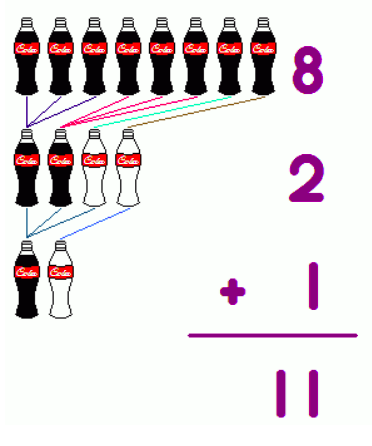
\includegraphics[scale=0.6]{images/cola.png} 
\end{center}
\end{figure}

Dê uma definição recursiva para a função $coca(n,m)$ que devolve o número de garrafas que você pode beber considerando que você tem $n$ garrafas cheias e $m$ garrafas vazias.



Primeiramente, vamos considerar os casos mais simples da função $coca(n,m)$:
$$coca(n,m) = 
\begin{cases}
0 & \text{, $m \leq 2 \wedge n = 0$}\\
n & \text{, $n \leq 2 \wedge m = 0$} 
\end{cases}
$$

Quando o número de garrafas vazias for menor ou igual a 2 e o número de garrafas cheias for zero não bebemos nenhuma garrafa. Quando o número de garrafas cheias for menor ou igual a 2 e o número de garrafas vazias for zero, bebemos apenas as garrafas cheias. 

Agora vamos considerar os casos mais complexos, vamos separar em dois casos:

$$coca(n,m) = 
\begin{cases}
coca(0, n+m) & \text{, $n \geq 0$}\\
coca(\lfloor m/3 \rfloor ,m \textbf{ mod } 3) & \text{, caso contrário} 
\end{cases}
$$

\end{exemplo}


\begin{exemplo}
3 objetos distintos podem ser organizados em sequência de seis maneiras diferentes.

\begin{center}
\begin{tabular}{c}
A,B,C\\
A,C,B\\
B,A,C\\
B,C,A\\
C,A,B\\
C,B,A\\
\end{tabular}
\end{center}

Dê uma definição recursiva para a função $f(n)$ que devolve o número de maneiras que podemos organizar n objetos distintos em sequência.

Seja f(n) o número de maneiras que podemos organizar n objetos distintos em uma sequência de tamanho $n$. O primeiro elemento de uma sequência pode ser escolhido de $n$ maneiras restando $n-1$ objetos para ser organizado em uma sequência de tamanho $n-1$. Logo,

$$
f(n) = 
\begin{cases}
1 & n = 1\\
n \cdot f(n-1) & \text{caso contrário}\\
\end{cases}
$$

\end{exemplo}

\begin{exemplo}



3 objetos distintos podem ser organizados em uma sequência de tamanho 2 de seis maneiras diferentes.

\begin{center}
\begin{tabular}{c}
A,B\\
A,C\\
B,A\\
B,C\\
C,A\\
C,B\\
\end{tabular}
\end{center}

Dê uma definição recursiva para a função $f(n, k)$ que devolve o número de maneiras que podemos organizar n objetos distintos em sequência de tamanho $k$ tal $k \leq n$.


Seja f(n,k) o número de maneiras que podemos organizar $n$ objetos distintos em uma sequência de tamanho $k$ tal que $k \leq n$. O primeiro elemento de uma sequência pode ser escolhido de $n$ maneiras restando $n-1$ objetos para ser organizado em uma sequência de tamanho $k-1$. Logo,

$$
f(n,k) = 
\begin{cases}
n & k = 1\\
n \cdot f(n-1,k-1) & \text{caso contrário}\\
\end{cases}
$$

\end{exemplo}

\begin{exemplo}{Números de triângulos em uma grade triangular}


\begin{minipage}{\textwidth}

Quantos triângulos em pé (tamanhos variados)
  podemos encontrar em uma grade de triângulos com
  altura $n$?
  
\begin{center}
    \begin{tikzpicture}
    \foreach \i in {0,1,2,3,4} {
      \draw (0 + 0.5*\i, \i * 0.5 * \sqrtofthree) -- (4 - 0.5*\i, \i * 0.5 * \sqrtofthree);
      \draw (0:\i) -- (60:\i);
      \draw[xshift=4cm] (180:\i) -- (120:\i);
    }
    \end{tikzpicture}
    \qquad
    \begin{tikzpicture}
    \fill[yellow!80] (0,0) -- (3,0) -- (1.5,3*0.5*\sqrtofthree);
    \fill[green!80] (1.5,0.5*\sqrtofthree) -- (3.5,0.5*\sqrtofthree) -- (2.5,3*0.5*\sqrtofthree);
    \foreach \i in {0,1,2,3,4} {
      \draw (0 + 0.5*\i, \i * 0.5 * \sqrtofthree) -- (4 - 0.5*\i, \i * 0.5 * \sqrtofthree);
      \draw (0:\i) -- (60:\i);
      \draw[xshift=4cm] (180:\i) -- (120:\i);
    }
    \end{tikzpicture}
  \end{center}

Destacamos dois triângulos de tamanhos variados encontrados em um triângulo de altura 4.

\end{minipage}


Seja $t(n)$ o número de triângulos em pé de tamanho variados que podemos encontrar em um grade triangulas com altura $n$.

Para uma grade de altura $n = 1$, temos $t(1) = 1$ triângulo

\begin{center}
    \begin{tikzpicture}
      \draw (0,0) -- (4,0) -- (2,4*0.5*\sqrtofthree) -- cycle;
    \end{tikzpicture}
  \end{center}
  
Para uma grade de altura $n = 2$, temos $t(2) = 4$ triângulo.

\begin{itemize}
  \item 2 com o vértice superior coincidindo com o vértice superior do maior triângulo.
  \item 2 outros triângulos com o vértice superior diferente do vértice superior do maior triângulo.
\end{itemize}

\begin{center}

\begin{tabular}{ll}

     \begin{tikzpicture}
      \foreach \i in {0,1,2} {
        \draw (0 + 1*\i, \i * 1 * \sqrtofthree) -- (4 - 1*\i, \i * 1 * \sqrtofthree);
        \draw (0:2*\i) -- (60:2*\i);
        \draw[xshift=4cm] (180:2*\i) -- (120:2*\i);
      }
      \draw[fill=blue!80] (1,\sqrtofthree) -- (3,\sqrtofthree) -- (2,2*\sqrtofthree) -- cycle;
      \draw[ultra thick, red!80] (0,0) -- (4,0) -- (2, 2*\sqrtofthree) -- cycle;
      \draw[ultra thick, red!80] (0,0) -- (4,0) -- (2, 2*\sqrtofthree) -- cycle;
    \end{tikzpicture}
&
         \begin{tikzpicture}
      \foreach \i in {0,1,2} {
        \draw (0 + 1*\i, \i * 1 * \sqrtofthree) -- (4 - 1*\i, \i * 1 * \sqrtofthree);
        \draw (0:2*\i) -- (60:2*\i);
        \draw[xshift=4cm] (180:2*\i) -- (120:2*\i);
      }
     
      \draw[fill=green!80] (0,0) -- (2,0) -- (1,\sqrtofthree) -- cycle;     
      \draw[fill=yellow!80] (2,0) -- (4,0) -- (3,\sqrtofthree) -- cycle;
      
    \end{tikzpicture}\\
\end{tabular}
  \end{center}

Podemos encontrar alguma padrão para $n=4$?

\begin{center}
    \begin{tikzpicture}
    
    
    
    
    \foreach \i in {0,1,2,3,4} {
      \draw (0 + 0.5*\i, \i * 0.5 * \sqrtofthree) -- (4 - 0.5*\i, \i * 0.5 * \sqrtofthree);
      \draw (0:\i) -- (60:\i);
      \draw[xshift=4cm] (180:\i) -- (120:\i);
    }
    \end{tikzpicture}
  \end{center}


Temos 4 triângulos têm o vértice superior coincidente com o vértice superior do triângulo maior

  \begin{center}
    \begin{tikzpicture}
      \fill[red!80]  (0,0) -- (4,0) -- (2, 2*\sqrtofthree) -- cycle;
      \fill[blue!80] (0.5,0.5 * \sqrtofthree) -- (3.5,0.5 * \sqrtofthree) -- (2, 4*0.5*\sqrtofthree) -- cycle;
      \fill[green!80] (1,\sqrtofthree) -- (3,\sqrtofthree) -- (2, 4*0.5*\sqrtofthree) -- cycle;
      \fill[yellow!80] (1.5,1.5*\sqrtofthree) -- (2.5,1.5*\sqrtofthree) -- (2, 4*0.5*\sqrtofthree) -- cycle;

      \foreach \i in {0,1,2,3,4} {
        \draw (0 + 0.5*\i, \i * 0.5 * \sqrtofthree) -- (4 - 0.5*\i, \i * 0.5 * \sqrtofthree);
      }
      \draw (0,0) -- (4,0) -- (2,4*0.5*\sqrtofthree) -- cycle;
    \end{tikzpicture}
  \end{center}
  
Os outros triângulos cujos vértices superiores não coincidem com o vértice superior do triângulo maior podem aparecer nesses dois triângulos amarelos internos (t(n-1)). Observe que somamos todos os triângulos que estão nos dois triângulos amarelos, os triângulos que estão dentro do triângulo vermelho (t(n-2)) serão contados duas vezes




\begin{center}
        \begin{tikzpicture}
          \foreach \i in {0,1,2,3,4} {
            \draw (0 + 0.5*\i, \i * 0.5 * \sqrtofthree) -- (4 - 0.5*\i, \i * 0.5 * \sqrtofthree);
            \draw (0:\i) -- (60:\i);
            \draw[xshift=4cm] (180:\i) -- (120:\i);
          }
          \draw[fill=yellow!80] (1,0) -- (4,0) -- (2.5, 3*0.5*\sqrtofthree) -- cycle;
          \draw[fill=yellow!80] (0,0) -- (3,0) -- (1.5, 3*0.5*\sqrtofthree) -- cycle;
          \draw[fill=red]  (1,0) -- (3,0) -- (2,   2*0.5*\sqrtofthree) -- cycle;
        \end{tikzpicture}
\end{center}

A definição recursiva de $t(n)$ é:
$$
t(n) =
\begin{cases}
1  & n = 1 \\
4  & n = 2 \\
n + 2 \cdot t(n-1) - t(n-2) & n \geq 3\\
\end{cases}
$$

\end{exemplo}


\begin{exemplo}

Ao subir a escada de seu prédio, José às vezes sobe dois degraus de uma vez e às vezes sobe um de cada
vez. Sabendo que a escada tem 3 degraus, de quantas maneiras diferentes José pode subir a escada? Você
consegue generalizar para o caso de uma escada com $n$ degraus?


Primeiramente, vamos pensar nos casos menores:

\begin{itemize}
    \item Uma escada de 1 degrau, podemos subir as escadas de 1 maneira (1).
    \item Uma escada de 2 degrau, podemos subir as escadas de 2 maneiras (1+1,2).
    \item Uma escada de 3 degraus, podemos subir as escadas de 3 maneiras (1+1+1,1+2,2+1).
\end{itemize}

Seja $x_n$ número de maneira de subir uma escada de $n$ degraus.  O primeiro passo para subir uma escada de n degraus pode ser dado de duas maneiras:

\begin{itemize}
    \item Se você subir apenas um degrau, então teremos $x_{n-1}$ maneiras de subir o restante da escada.
    \item Se você subir dois degraus, então teremos $x_{n-2}$ maneiras de subir o restante da escada.
\end{itemize}

A recorrência para $x_n$ será:

$$
x_n = \begin{cases}
1 & n = 1\\
2 & n = 2\\ 
x_{n-1} + x_{n-2} & n \geq 3\\
\end{cases}
$$
\end{exemplo}

\begin{exemplo}
Quantas são as sequências de n termos pertencentes a \{0,1\} , que possuem um número ímpar de termos iguais a 0?

Por exemplo,

Sequências de tamanho 1: 1 (0) 

Sequências de tamanho 2: 2 ( 01 e 10)

Encontre uma relação de recorrência que relaciona o número de termos dessa sequência.

Seja f(n) o número de sequências de $n$ termos 0 e 1 com uma quantidade ímpar de termos iguais a 0. O número de sequência de $n+1$ termos 0 e 1 com um número ímpar de termos iguais a 0 é igual a soma:
\begin{itemize}
    \item do número de sequências começadas por 1 seguido por uma sequência de $n$ termos com um número ímpar de zeros 
    \item com o número de sequências começadas por zero seguido por um sequência de $n$ termos com um número par de zeros.
\end{itemize}


Portanto,

\begin{equation}
    f(n+1) = f(n) + 2^n - f(n) = 2^n
\end{equation}

Logo,

\begin{equation}
    f(n)  = 2^{n-1}
\end{equation}

\end{exemplo}

\section{Exercícios}


\begin{enumerate}
\item 



Suponha que um par de coelhos recém-nascidos, um macho e uma fêmea, sejam colocados em um campo. Os coelhos podem acasalar com um mês de idade, de modo que no final do segundo mês uma fêmea pode produzir outro casal de coelhos. Suponha que nossos coelhos nunca morram e que a fêmea sempre produz um novo par (um macho, uma fêmea) a cada mês a partir do segundo mês.  

\begin{center}
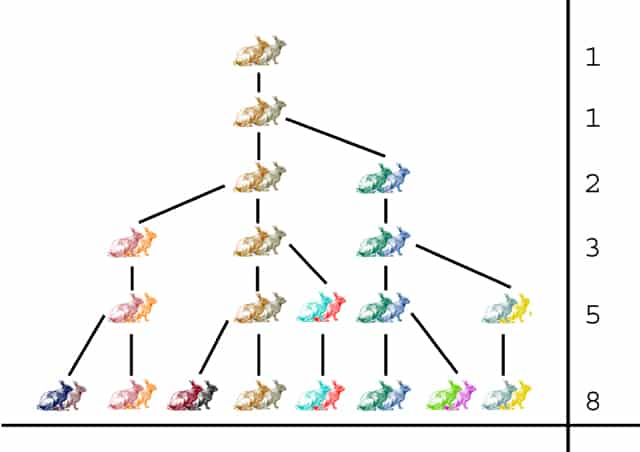
\includegraphics[scale=0.4]{images/rabbits.jpg} 
\end{center}

A imagem mostra que ao final do sexto mês teremos 8 pares de coelhos.


Quantos pares de coelhos teremos ao final de n meses?

Desenvolva uma função recursiva $f(n)$ que devolve o número de pares de coelhos após $n$ meses.

\item 




Suponha agora os nossos coelhos não vivam para sempre e morrem depois de k meses. Contudo, os coelhos acasalam com um mês de idade e cada fêmea produz um novo par de coelhos a cada mês a partir do segundo mês.


\begin{center}
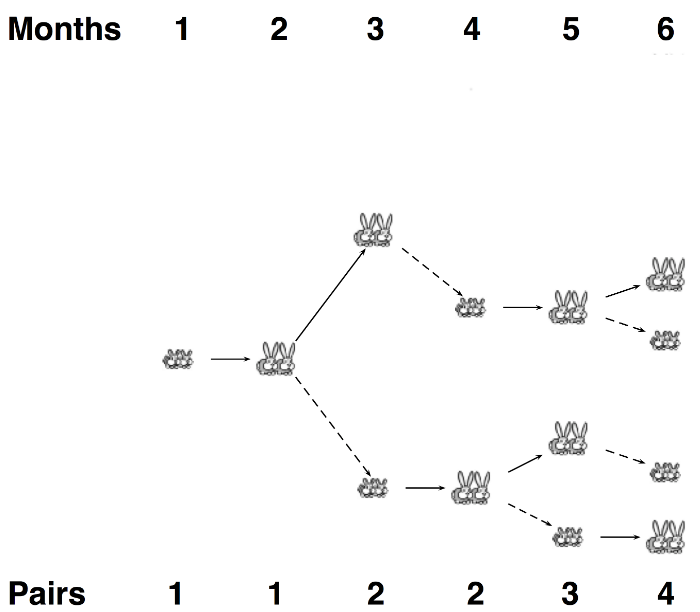
\includegraphics[scale=0.4]{images/rabbits2.png} 
\end{center}

A imagem mostra que ao final de seis meses teremos apenas 4 pares de coelhos considerando que os coelhos morrem após 3 meses.

Quantos pares de coelhos teremos ao final de n meses?

Desenvolva uma função recursiva $f(n,k)$ que devolve o número de pares de coelhos após $n$ meses considerando que os coelhos morrem depois de k meses. 



\item 

Ao subir a escada de seu prédio, José  sobe 1, 2 ou 3 degraus de uma vez. Sabendo que a escada tem 5 degraus, de quantas maneiras diferentes José pode subir a escada? Você
consegue generalizar para o caso de uma escada com $n$ degraus?

\item 

Quantas são as sequências de n termos pertencentes a \{0,1,2\} , que não possuem dois zeros consecutivos?

Por exemplo,

Sequências de tamanho 1: 3 (0,1 e 2) 

Sequências de tamanho 2: 8 ( 01,02,10,11,12,20,21 e 22)

\item 

Quantas são as sequências de n termos pertencentes a \{0,1,2\} , que não possuem dois zeros consecutivos?

Por exemplo,

Sequências de tamanho 1: 3 (0,1 e 2) 

Sequências de tamanho 2: 8 ( 01,02,10,11,12,20,21 e 22)

Faça um programa que gere todas as sequências de tamanho $n$ com termos pertencentes  a \{0,1,2\} , que não possuem dois zeros consecutivos.


\item 

Quantas são as sequências de n termos pertencentes a \{0,1,2\} , que possuem um número ímpar de termos iguais a 0?

Por exemplo,

Sequências de tamanho 1: 1 (0) 

Sequências de tamanho 2: 4 ( 01, 10, 20 e 02)

Encontre uma relação de recorrência que relaciona o número de termos dessa sequência.

\item 

Renata montou uma sequência de triângulos com palitos de fósforo, seguindo o padrão indicado na figura abaixo.

\begin{center}
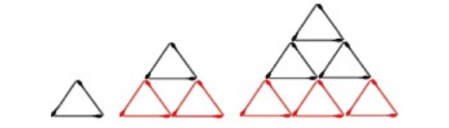
\includegraphics[width=1.0\linewidth,scale=0.8]{images/palitos.png} 
\end{center}

Quantos palitos serão usados por Renata no n-ésimo termo dessa sequência?

\item
Começando com um quadrado de 1cm de lado, formamos uma sequência de figuras, ob-
serve a figura abaixo. Cada figura, a partir da segunda, é formada unindo-se três cópias
da anterior. Os contornos destacados em vermelho das quatro primeiras figuras medem,
respectivamente, 4cm, 8cm, 20cm e 56cm. Quanto mede o contorno da figura n?


\begin{center}
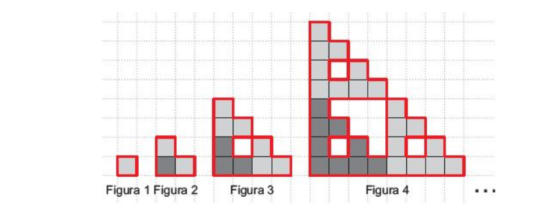
\includegraphics[width=1.0\linewidth,scale=0.8]{images/figura_recursiva.png} 
\end{center}

\item 

Um convidado em uma festa é uma celebridade se essa pessoa for conhecida por todos os outros convidados, mas não conhece nenhum deles. Existe no máximo uma celebridade em uma festa, pois se houvesse duas, eles se conheceriam.. Uma festa particular pode não ter celebridade. Sua tarefa é encontrar a celebridade, se ela
existe, em uma festa, fazendo apenas um tipo de pergunta - perguntando a um convidado se ele conhece um segundo convidado. Todos devem responder às suas perguntas com sinceridade. Ou seja, se Alice e Bob são duas pessoas na festa, você pode perguntar a Alice se ela conhece Bob; ela deve responder corretamente.

Seja $G(n)$ o número de perguntas utilizada para encontrar uma celebridade em uma festa com n pessoas.

\begin{enumerate}
    \item Calcule $G(1)$, $G(2)$, $G(3)$
    \item Proponha uma definição recursiva para $G(n)$. [Dica: primeiro faça uma pergunta para eliminar uma pessoa como celebridade. Em seguida, identifique  uma celebridade em potencial. Por fim, faça mais duas perguntas para determinar se a celebridade em potencial é na verdade uma celebridade.]
\end{enumerate}


\item 

Suponha que existem $n$ pessoas em um grupo, cada pessoa está ciente de um escândalo que
ninguém mais no grupo sabe sobre. Essas pessoas conversam por telefone; quando duas pessoas no grupo conversam, elas compartilham informações sobre todos os escândalos que cada um conhece. Para
por exemplo, na primeira chamada, duas pessoas compartilham informações, então
ao final da ligação, cada uma dessas pessoas sabe sobre dois escândalos. O problema da fofoca pede $G(n)$, o mínimo número de chamadas telefônicas necessárias para todas as n pessoas para
aprenda sobre todos os escândalos. 

\begin{enumerate}
    \item Mostre $G(1) = 0$
    \item Mostre $G(2) = 1$
    \item Mostre $G(3) = 3$
    \item Mostre $G(4) = 4$
    \item Mostre $G(5) = 6$
    \item Proponha um definição recursiva para $G(n)$
    
    
\end{enumerate}

\end{enumerate}













\section{Algoritmo Recursivo}

Um algoritmo é dito recursivo quando ele resolve um problema reduzindo para uma instância do mesmo problema com uma entrada menor.

\begin{exemplo}{Exponenciação}

Considere a seguinte definição recursiva da exponenciação:

\begin{equation}
a^n = 
\begin{cases}
1           & , n = 0\\
a * a^{n-1} & , n \geq 1
\end{cases}
\end{equation}
\end{exemplo}
O algoritmo recursivo para calcular $a^n$:

\begin{minted}{C++}
int exp(int a, int n){
	if(n==0) return 1;
	else return a*exp(a, n-1);
}
\end{minted}



No algoritmo acima, realizamos $n-1$ multiplicações para calcular $a^n$. Podemos fazer melhor utilizando uma outra definição recursiva.


\begin{exemplo}{Exponenciação rápida}

\begin{equation}
a^n = 
\begin{cases}
1           & , n = 0\\
(a^{n/2})^2 & , \text{$n$ é par}\\
a * a^{n-1} & , \text{$n$ é ímpar}

\end{cases}
\end{equation}
\end{exemplo}
\begin{minted}{C++}
int fast_exp(int a, int n){
    if(n==0) return 1;
    if(n%2==0){
        int res = fast_exp(a,n/2);
        return res*res;
    }else{
        return a*fast_exp(a, n-1);
    }
    
}
\end{minted}




\begin{exemplo}{soma de um vetor}

A definição recursiva da soma dos elementos de um vetor $a$ com índices variando entre $start$ e $end$:

\begin{equation}
soma(a, start, end) = 
\begin{cases}
a[start]           & , start = end\\
a[start] + soma(a, start+1, end) & , \text{caso contrário}\\

\end{cases}
\end{equation}


O algoritmo recursivo para calcular a soma dos elementos entre os duas posições start e end.

\begin{minted}{C++}
int soma_vetor(int *a, int start, int end){
	if( start == end ){
		return a[start];
	}else{
		return a[start] + soma_vetor(a, start + 1, end);
	}
}
\end{minted}

\end{exemplo}

\begin{exemplo}{Palavra palíndroma}

Considere a definição recursiva da função $is\_palindrome(s,i,j)$  que verificar se um palavra $s[i\ldots j]$ é palíndroma :

\begin{equation}
is\_palindrome(a, start, end) = 
\begin{cases}
true , start > end\\
true , start = end\\
s[start] == s[end] \&\& is\_palindrome(s, start+1, end-1)  \text{, caso contrário}\\

\end{cases}
\end{equation}




Observe que para testar se uma palavra com tamanho maior ou igual a 2, precisamos testar se o primeiro e o último caractere são iguais, depois precisamos testar se a palavra obtida pela remoção do primeiro e do último caractere  também é palíndroma.

\begin{minted}{C++}
bool is_palindrome(char s[], int i, int j){
    
    //palavra vazia
    if( i  > j ) return true;  
    //palavra de tamanho 1
    if( i == j ) return true; 
    
    if( s[i] == s[j] )
        return is_palindrome(s, i+1, j-1);
    else
        return false;
    
}
\end{minted}

\end{exemplo}


\begin{exemplo}{Busca linear}

Dado um vetor não-ordenado de inteiros de tamanho $n$ ( $a_0,a_1, \ldots, a_{n-1}$) e um um inteiro x. Implemente a função $busca(a, i, j, x)$ que devolve o índice da primeira ocorrência de x no subvetor $a_i, a_{i+1}, \ldots, a_j$, caso contrário, devolve -1. 

A função $busca(a, i, j, x)$ pode ser definida recursivamente da seguinte maneira:

\begin{equation}
busca(a, i, j , x) = 
\begin{cases}
  i, \text{se } A[i] = x\\
 -1, \text{se } i == j \\
busca(a, i+1, j, x) \text{, caso contrário}\\

\end{cases}
\end{equation}

\begin{minted}{C++}
int busca( int * A, int i, int j, int x){
    if( A[i] == x ) return i;
    else if(i == j) return -1;
    else return busca(A, i+1, j, x);
}
\end{minted}


\end{exemplo}

\begin{exemplo}
Dado um vetor de inteiros $arr$ de tamanho n existe uma posição k tal que 

$$arr[0] < arr[1] < ... < arr[k] > arr[k+1] > arr[k+2] > ... > arr[n-1]$$

Descubra $k$ usando a busca binária.

A função $pico(a, p, r)$ que devolve o valor de $k$ no intervalo $[p,r]$ pode ser definida recursivamente

\begin{equation}
pico(A, p, r) = 
\begin{cases}
  p  & \text{, se } p = r\\
  max(A[p],A[r]) & \text{, se } r == p+1 \\
  mid & \text{,} A[mid] > A[mid-1] \text{ e } A[mid] > A[mid+1]  \\
  pico(A, mid+1,r)      & \text{,} A[mid] < A[mid+1] \text{ e } A[mid-1] < A[mid]   \\
  pico(A, p,mid-1)      & \text{,} A[mid-1] > A[mid]    \\
\end{cases}
\nonumber 
\end{equation}
onde mid = (p+r)/2;


\begin{minted}{C++}
int pico(vector <int> & A, int p, int r){
    if( r-p == 0 ){ // tamanho 1
        return p;
    }else if( r-p == 1){ // tamanho 2 
        if(A[p] > A[r]) return p;
        else return r;
    }else{ // tamanho 3 ou mais
        int mid = p+r/2;
        if(A[mid] > A[mid-1] && A[mid] > A[mid+1]) return mid;
        if( A[mid-1] < A[mid]){
            if( A[mid] > A[mid+1] ) return mid;
            else{ // A[mid] < A[mid+1]
                return pico(A, mid+1, r);
            }
        }else{ // A[mid-1] > A[mid]  
            return pico(A, p, mid-1);
        }    
    }
}

\end{minted}
    
\end{exemplo}



\section{Exercícios}

\begin{enumerate}
    \item Proponha um algoritmo recursivo para encontrar o máximo de um vetor de tamanho $n$ usando o fato que o máximo de n inteiros é o maior entre o último inteiro do vetor e o máximo dos primeiros n-1 inteiros do vetor. 
    
    \item Proponha um algoritmo recursivo para computar o maior divisor comum de dois inteiros não negativos $a$ e $b$ com a  < b usando o fato que $mdc(a,b) = mdc(a, b-a)$. Note que se um número $d$ divide $a$ e $b$ então ele divide $a$ e $b-a$.
    
    \item Proponha um algoritmo recursivo para encontrar a primeira ocorrência de um valor x em um vetor ordenado de tamanho $n$ ( $a_0,a_1, \ldots, a_{n-1}$). Implemente a função $busca(a, i, j, x)$ que procura a primeira ocorrência de x no subvetor $a_i, a_{i+1}, \ldots, a_j$. 
    
    \item Proponha um algoritmo recursivo para multiplicar dois inteiros não-negativos baseado no fato que $x \cdot y = 2 \cdot (x \cdot y/2)$ quando $y$ é par e $x \cdot y = 2( x \cdot \lfloor y / 2 \rfloor) + x$ quando $y$ é ímpar, juntamente com a condição inicial que $x \cdot y = 0$ quando $y = 0$ 
    
    \item Proponha um algoritmo recursivo para computar $n^2$ para todo n inteiro não negativo usando o fato que $(n+1)^2 = n^2 + 2n + 1$.
    
    \item Seja $A = \{a^ib^i| i \in \mathbb{N}\}$ um conjunto de palavras. Proponha um algoritmo que recebe uma palavra $s$ de tamanho $n$ e verifica se $s \in A$. Dica: faça um função $check(s, 0, n-1)$ que verifica que se $s[0\ldots n-1]$ pertence ao conjunto  $A$.
    
    \item Seja $A = \{a^ib^ia^jb^j| i,j \in \mathbb{N}\}$ um conjunto de palavras. Proponha um algoritmo que recebe uma palavra $s$ de tamanho $n$ e verifica se $s \in A$. Dica: faça um função $check(s, 0, n-1)$ que verifica que se $s[0\ldots n-1]$ pertence ao conjunto  $A$.
    
    
    %\item Proponha um algoritmo recursivo que recebe dois vetores ordenados de tamanho $n$ e $m$ e devolve um vetor ordenado de tamanho $n+m$ com os elementos dois vetores dados. 
    
    \item Escreva uma função recursiva que calcule a soma dos dígitos decimais de um inteiro positivo.
Por exemplo, a soma dos dígitos de 132 é 6.

    \item O coeficiente binomial é uma relação estabelecida entre dois números naturais $n$ e $k$, $n\geq k\geq 0$, indicada por:

\begin{equation}
\binom{n}{k} = \frac{n!}{k!(n-k)!}  
\end{equation}   


Escreva uma função recursiva que calcule o coeficiente binomial de dois números inteiros não negativos $n$ e $k$, $n\geq k$.
 
Dica: Use a relação de Stifel:

\begin{equation}
\binom{n-1}{k-1} + \binom{n-1}{k} = \binom{n}{k}
\end{equation}



\item Uma sequência do gray code de n bits é uma sequência de $2^n$ inteiros onde:

\begin{itemize}
\item Cada número inteiro está no intervalo inclusivo [0, $2^n - 1$],
\item O primeiro inteiro é 0,
\item Um número inteiro aparece no máximo uma vez na sequência,
\item A representação binária de cada par de inteiros adjacentes difere em exatamente um bit, e
\item A representação binária do primeiro e do último inteiro difere exatamente um bit.
\end{itemize}

Dado um inteiro n, retorna qualquer sequência de gray code de n bits válida.

\begin{center}
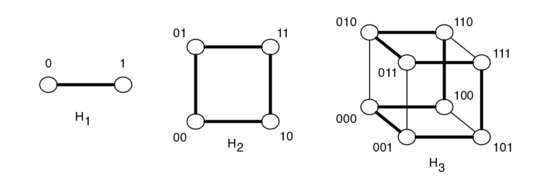
\includegraphics[scale=0.8]{images/hipercubo.png} 
\end{center}

\item Três marinheiros naufragaram em uma ilha e eles coletaram uma grande pilha de cocos durante o dia. Naquela noite, o primeiro marinheiro acorda e decide pegar sua primeira porção mais cedo, então tenta dividir a pilha de cocos igualmente em três pilhas, mas descobre que sobrou um coco, então ele o joga para um macaco e depois esconde sua parte das três pilhas de cocos do mesmo tamanho e junta as outras duas pilhas juntas para formar uma única pilha visível de cocos novamente e vai para a cama.

Para encurtar a história, cada um dos marinheiros, por sua vez, se levanta uma vez durante a noite e executa as mesmas ações de dividir a pilha de coco em três, descobrindo que sobrou um coco e dando aquele único coco restante ao macaco.

Pela manhã (após a ação clandestina e separada de cada um dos cinco marinheiros durante a noite), os cocos restantes são divididos em três pilhas iguais para cada um dos marinheiros, após o que se verifica que a pilha de cocos se divide igualmente entre os marinheiros sem resto. (Nada para o macaco pela manhã.)

Faça um programa que dado um inteiro N representando o número inicial de marinheiros encontre o número piha de cocos coletadas inicialmente. 

\textbf{Entrada}

Uma linha contendo um inteiro (N  $\leq$ 9 ) representando o número de marinheiro.

\textbf{Saída}

Devolva um inteiro representando o número de coco coletados inicialmente.\\

\textbf{Entrada}\\
3\\

\textbf{Saída} \\
25\\

\item \textbf{TapiocaSort} Preparar a pilha perfeita de tapiocas é uma tarefa complicada, porque não importa como você tenta todas as tapiocas em qualquer pilha têm diâmetros diferentes. Para o bem da limpeza, no entanto, você pode ordenar a pilha por tamanho de forma que cada tapioca seja menor do que todos os panquecas abaixo dela. O tamanho de uma panqueca é dado pelo seu diâmetro.

A ordenação de uma pilha é feita por uma sequência de "viradas" de tapiocas. Uma virada consiste em inserir uma espátula entre duas tapiocas em uma pilha e virando (invertendo) todas as panquecas em a espátula (invertendo a subpilha).

Uma virada é especificado dando a posição da tapioca na parte inferior da subpilha a ser virada em relação a toda a pilha. A panqueca de baixo tem a posição 1, enquanto a panqueca de cima em uma pilha de n panquecas tem posição n.

Uma pilha é especificada dando o diâmetro de cada tapioca na pilha na ordem em que aparecem as tapiocas. Por exemplo, considere uma pilha de tapiocas abaixo em que a tapioca 5 é a primeira tapioca do vetor:

topo -> 5 1 2 3 4 |

Fazendo a operação virada 1 (a espátula está representada por |), obtemos a seguinte pilha de tapiocas:

topo -> 4 3 2 1 | 5

Fazendo a operação virada 2, obtemos a seguinte pilha de tapiocas:

topo -> 1 2 3 4 5

Observe que a pilha de tapioca pode ser ordenada utilizando duas operações de virada.

\textbf{Entrada}

A primeira linha da entrada contém um inteiro N representando o número de tapiocas.

A segunda linha contém N inteiros positivos representando uma pilha de tapiocas. Cada tapioca terá um diâmetro entre 1 e 30.

\textbf{Saída}

Seu programa deve imprimir uma sequência de viradas que resulte na pilha de tapioca ordenada de maneira que a maior tapioca está na parte inferior e a menor tapioca na parte superior. A sequência de viradas deve terminar com 0, indicando que não são mais necessárias viradas.


\begin{tabular}{|l|l|}
\hline
Exemplo de Entrada & Exemplo de Saída\\
5                & 1 2 0\\      
5 1 2 3 4        &\\
\hline
\end{tabular}


\begin{tabular}{|l|l|}
\hline
Exemplo de Entrada & Exemplo de Saída\\
5                & 1 0\\      
5 4 3 2 1        &\\
\hline
\end{tabular}

\item  Pão a metro é um tipo de sanduíche gigante que é uma excelente opção de lanche para torneios de programação, embora a experiência já tenha mostrado que o oferecimento de sanduiches pode gerar reclamação dos competidores. Outro grande problema é que algumas pessoas são mais gulosas que outras e, dessa maneira, acabam pegando pedaços maiores que os pedaços dos outros. Para a final da OBI, a coordenação estava pensando em providenciar pão a metro para os competidores, porém tais problemas os fizeram recuar na idéia.

Embora a idéia tenha sido momentaneamente abandonada, uma idéia simples surgiu: cortar previamente o pão em fatias de tamanho iguais e distribuí-las entre as pessoas. O único problema com tal idéia é que se o número de pessoas for muito grande, fica impraticável ter apenas um pão. Por exemplo, se quisermos que 1.000 pessoas recebam 20 centímetros de sanduíche, seria necessário um sanduíche de 20.000 centímetros, ou 200 metros!

Alguém levantou a seguinte hipótese: se houvesse N pessoas e fossem encomendados K sanduíches de empresas diferentes, cada qual com uma determinada metragem (tamanho) $M_i$ ($1 \leq i \leq K$), seria possível retirar desses pães N fatias de mesmo tamanho, possivelmente sobrando partes nao utilizadas. A questão seria: qual o tamanho inteiro máximo que essas fatias poderão ter?

Por exemplo, se tivermos K = 4, com os tamanhos (em centímetros) M1 = 120, M2 = 89, M3 = 230 e M4 = 177 e N = 10, podemos retirar N fatias iguais de tamanho máximo 57, pois assim conseguimos 2 fatias no primeiro pão, 1 no segundo, 4 no terceiro e 3 no quarto, totalizando as 10 fatias necessárias. Se tentarmos cortar fatias de tamanho 58, só será possível obter 3 fatias do terceiro pão, totalizando 9 e, portanto, 57 é realmente o melhor que podemos obter. Note que não podemos usar duas ou mais fatias menores de diferentes pães para formarmos uma fatia do tamanho selecionado. (ficaria muito deselegante dar um lanche recortado às pessoas).

Tarefa

Escreva um programa que, dados os tamanhos de pão disponíveis (em centímetros) e a quantidade de pessoas a serem atendidas, retorne o tamanho inteiro máximo (em cent ímetros) da fatia que pode ser cortada de maneira a atender todas as pessoas.

Entrada

A entrada contém um único conjunto de testes, que deve ser lido do dispositivo de entrada padrão (normalmente o teclado). A primeira linha da entrada contém um inteiro N que indica a quantidade pessoas ($1 \leq N \leq 10.000$). A segunda linha contém um inteiro K ($1 \leq K \leq 10.000$) que é a quantidade de sanduíches disponível. Na terceira linha há K inteiros M ($1 \leq M \leq 10.000$) separados por um espaço em branco representando o tamanho de cada pão.

Saída Seu programa deve imprimir, na saída padrão, uma única linha, contendo o tamanho inteiro máximo da fatia que pode ser cortada.

Exemplos


\begin{tabular}{|l|l|}
\hline
Entrada & Saída\\
\hline
10                & 57\\      
4        &\\
120 89 230 77 & \\
\hline
\end{tabular}


    
\end{enumerate}




















\section{Backtracking}

O algoritmo de backtracking pode ser entendido como um refinamento de um algoritmo de força bruta. No algoritmo de backtracking, a solução para um problema computacional é construída de maneira incremental assim que uma condição do problema é violada, o algoritmo retrocede e tenta a próxima alternativa.

Vamos exemplificar o funcionamento de um algoritmo de backtracking na solução de um problema de satisfação. Um problema de satisfação pode ser definido por uma tripla $(X, D, C)$ onde:

\begin{itemize}
    \item $X = \{X_1, X_2, \ldots, X_n\}$ é um conjunto de variáveis.
    \item $D = \{D_1, D_2, \ldots, D_n\}$ é o conjunto dos respectivos domínios de cada variável.
    \item $C = \{C_1,C_2, \ldots,C_m\}$ é o conjunto de restrições do problema.
\end{itemize}


\begin{algorithm}
  \caption{Algoritmo de Backtracking}\label{AIPal}
  \begin{algorithmic}
    \Function{Backtracking}{$i,n$}
    
    \If{i = n+1}
        \State save\_solution(X)
    \Else 
        \For{$j \in D_i$}
            \If{$X[i] = j$ não viola nenhuma restrição}
            \State X[i] $\leftarrow$ j
            \State Backtracking(i+1, n)
            \EndIf
        \EndFor
    \EndIf
     
    \EndFunction
  \end{algorithmic}
\end{algorithm}

\subsection{Problema das n rainhas}

No problema das $n$ rainhas, temos n variáveis $(Q[1],Q[2], \ldots, Q[n])$. Cada variável $Q[i]$ guarda a posição da linha da i-ésima rainha. Em tabuleiro $n \times n$, $Q[i] \in \{1, 2, \ldots, n\}$. Neste problema, temos $n$ variáveis e seus domínios tem $n$ valores distintos.  As restrições para o problema são as seguintes:

\begin{enumerate}
    \item $\forall { 1 \leq  i < j \leq n} \quad Q[i] \neq Q[j] $
    \item $\forall { 1 \leq  i < j \leq n} \quad Q[i] + i \neq Q[j] + j$.
    \item $\forall { 1 \leq  i < j \leq n} \quad Q[i] - i \neq Q[j] - j$.
\end{enumerate}

A restrição (1) garante que não teremos duas rainhas distintas na mesma linha. A restrição (2) garante que não teremos duas rainhas na mesma diagonal secundária. A restrição (3) garante que não teremos duas rainhas na mesma diagonal principal. 

No algoritmo de backtracking, essas restrições são verificadas de maneira incremental considerando as fixações das variáveis já realizadas.

O Código abaixo escrito em C++ implementa o algoritmo de backtracking para o problema da n rainhas descrito acima.

\begin{minted}{C++}
void place_queen(vector <int> Q, int r, int n, int & cont){
    if(r == n+1){
        cont++;
    }else{
        for(int j = 1; j <= n; j++){
            bool legal = true;
            for(int i = 1; i <= r-1; i++){
                if( Q[i] == j || Q[i] == j+r-i || Q[i] == j-r+i){
                    legal = false;
                }
            }
            if(legal){
                Q[r] = j;
                place_queen(Q, r+1, n, cont);
            }
        }
    }
}

\end{minted}

\subsection{Problema da soma de subconjuntos}

Dado um conjunto $S$ com $n$ elementos encontre um subconjunto $S' \subseteq S$ tal que a soma dos elementos de $S'$ seja igual a um valor $K$.

Esse problema pode ser modelado da seguinte maneira. Teremos $n$ variáveis $(X[1], X[2], \ldots, X[n])$. Cada variável X[i] pode assumir dois valores \{true, false\}. Se X[i] é true, então $S[i] \in S'$. Caso contrário $S[i] \not \in S'$.

O nosso problema terá uma única restrição:

\begin{itemize}
    \item $\sum_{i=1}^{n} X[i]\cdot S[i] = K$
\end{itemize}

O Código abaixo escrito em C++ implementa o algoritmo de backtracking para o problema da soma de subconjunto.

\newpage 

\begin{minted}{C++}
void subsetsum(vector <int> & S,vector <bool> X, int K, int i, int n){
    if(i == n){
        bool flag = true;
        cout << "{";
        for(int j = 0; j < i; j++){
            if(X[j])
                cout << S[j] << " ";
        }
        cout << "}" << endl;
    }else{
        int prev = 0;
        for(int j = 0; j < i; j++){
            if(X[j])
                prev += S[j];
        }
        
        int next = 0;
        for(int j = i+1; j < n; j++){
            next += S[j];
        }

        
        if(prev + next >= K){            
            X[i] = false;
            subsetsum(S, X, K,  i+1, n);
        }
        
        if(prev + S[i] <=  K){
            X[i] = true;
            subsetsum(S, X, K, i+1, n);
        }
    }
}

int main(){
    
    vector <int> S( {2,3,4,1,7,8});
    vector <bool> X;
    X.resize(S.size());
    int K = 5;
    subsetsum(S, X, K, 0, S.size());
}

//Output:
//{4 1 }
//{2 3 }

\end{minted}

\subsection{Exercícios}

\begin{enumerate}
\item 

No quebra-cabeças Unruly, você recebe um tabuleiro $n \times n$. Cada quadrado do tabuleiro é colorido inicialmente com as cores branco, preto e cinza. O objetivo do jogo é pintar cada quadrado com a cor cinza com preto ou branco, de forma que:

\begin{itemize}
    \item não há três quadrados consecutivos, horizontalmente ou verticalmente, são da mesma cor
    \item cada linha e coluna contém o mesmo número de quadrados pretos e brancos. 
\end{itemize}

\begin{center}
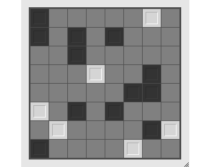
\includegraphics[scale=0.8]{images/unruly.png} 
\end{center}

Desenvolva um algoritmo de backtracking que resolva esse quebra-cabeça.

O jogo pode ser encontrado no seguinte link: \url{https://www.chiark.greenend.org.uk/~sgtatham/puzzles/js/unruly.html}

\item No quebra-cabeças Rectangles, você recebe uma grade retangular e alguns quadrados numerados.

\begin{center}
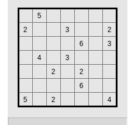
\includegraphics[scale=1.0]{images/Rectangles.png} 
\end{center}

Seu objetivo é traçar linhas paralelas as bordas grade rectangular para dividir a grade em retângulos, de modo que cada retângulo contenha exatamente um quadrado numerado e sua área seja igual ao número escrito naquele quadrado.

\begin{center}
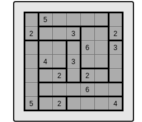
\includegraphics[scale=1.0]{images/Rectangles2.png} 
\end{center}

O jogo pode ser encontrado no seguinte link: \url{https://www.chiark.greenend.org.uk/~sgtatham/puzzles/js/rect.html}


\end{enumerate}






%\subsection{Maior subsequência crescente (Longest Increasing Subsequence)}

%Dado um vetor inteiro $A[1..n-1]$, nós precisamos encontrar a maior sequência de índices $i_1,i_2, \ldots, %i_l$ tal que $1 \leq i_1 < i_2 < \ldots < i_l \leq n$ e $A[i_1] < A[i_2] < \ldots < A[i_l]n$ 




% \section{Definição recursivas de conjuntos}

% Alguns conjuntos podem ser definidos de maneira recursiva. O conjuntos dos números pares positivos $P$ pode ser definido recursivamente da seguinte maneira:

% \begin{itemize}
%     \item $0 \in P$
%     \item Se $n \in P$ eentão $n+2 \in P$.
% \end{itemize}


% %Considere uma definição alternativa do conjuntos dos números pares positivos de maneira explicíta: 
% %\begin{equation}
% %P' = \{ 2k | k \in \mathbb{N} \}    
% %\end{equation}

% %É fácil mostrar que $P = P'$. 

% Seja S o conjunto dos pares ordenados de inteiros positivos $(a,b)$ tal que $2 | a + b$ pode ser definido recursivamente da seguinte maneira:

% \begin{itemize}
%     \item Passo Base: $(0,0) \in S$
%     \item Passo Recursivo Se $(a,b) \in S$ então $(a+1,b+1),(a+2,b),(a,b+2) \in S$.
% \end{itemize}

% O conjunto de todos os subconjuntos de um conjunto A, $subsets(A)$, pode ser definido recursivamente da seguinte maneira:

% \begin{itemize}
%     \item Passo Base: $\emptyset \in subsets(A)$
%     \item Passo Recursivo Seja $x \in A$, $Y \in subset(A\setminus \{x\})$ então $Y, Y \cup \{x\} \in subsets(A)$.
% \end{itemize}












%%
\chapter{Análise de algoritmos}
\label{chapter:typesetting}


\epigraph{
“Um bom algoritmo, mesmo rodando em uma máquina lenta, sempre
acaba derrotando (para instâncias grandes do problema) um algoritmo
pior rodando em uma máquina rápida. Sempre.”

\textit{— S. S. Skiena, The Algorithm Design Manual}
}

\epigraph{

Um cientista americano perguntou para um cientista russo: Quando vocês desenvolveram a bomba atômica, como você conseguiram executar uma grande quantidade de cálculo com seus computadores fracos?. O cientista russo respondeu: "Nós desenvolvemos algoritmos melhores"
Anedota russa
}

Muitos fatores podem influenciar o tempo de execução de algoritmo. Inicialmente, precisamos de um modelo que seja genérico e independente da máquina/linguagem usada. 

No modelo Máquina de acesso aleatório (Random Access Machine  - RAM), consideramos as seguintes hipóteses:

\begin{itemize}
    \item As instruções são executadas uma após a outra, sem operações concorrentes.
    \item Cada operação simples (+,-,*,/,if) demora um 1 passo.
    \item Cada acesso à memória custa também um passo.
    \item As operações realizadas com dados inteiros e ponto flutuantes tem o mesmo custo.
\end{itemize}

Algumas implicações da adoção desse modelo:

\begin{itemize}
    \item A hierarquia de memória dos computadores é desprezada.
    \item A utilização de paralelismo também é desprezada.
\end{itemize}


\section{Analisando número de operações de um programa}

Considere o seguinte programa que dado um vetor de inteiros de tamanho $n$ conta o número de elementos iguais a zero.

\begin{lstlisting}[language=C, caption={primeiro programa}]
int count = 0;
for ( int i=0; i<n; i++)
    if (v[i] == 0) count++;
\end{lstlisting}

Contando o número de operações simples:

\begin{tabular}{|l|l|}
\hline
Operações & Número de operações\\
\hline
Declaração de variáveis & 2\\
\hline
Atribuições &  2\\
\hline
Comparação "menor que" & n+1\\
\hline
Comparação "igual a" & n\\
\hline
Acesso a um elemento do vetor & n\\
\hline
Incremento & entre n e 2n\\
\hline
\end{tabular}

Observe que o número de operações depende da instância de entrada do problema. O número de passos com relação ao tamanho da entrada será descrita pela função $T(n)$:


No pior caso, o número de operações será:

$$
T(n) = 2 + 2 + (n+1) + n+ n + 2n = 5n + 5
$$

No melhor caso, o número de operações será:

$$
T(n) = 2 + 2 + (n+1) + n+ n + n = 4n + 5
$$

Observe que o processo de análise de algoritmo, pode ser uma tarefa árdua se consideramos todas as operações simples envolvidas. Em geral, escolhemos a operação mais executada e contamos apenas quantas vezes ela está sendo executada. No exemplo acima, poderíamos ter analisado apenas o número de vezes que a operação de incremento está sendo executado.

Agora, iremos analisar o algoritmo de ordenação por inserção:

\begin{minted}{C++}
    int x, i; //2 declaracao
    // 1 declaracao, 1 atribuicao, n comparacoes, n incrementos 
    for(int j = 1; j < n; j++){ 
        x = A[j]; // n-1 atribuicao
        i = j-1; // n-1 atribuicao
        //n-1 vezes o while
        while(i >= 0 && A[i] > x){ // entre 1 e j comparações  
            A[i+1] = A[i]; //entre 0 e j-1 vezes atribuições
            i = i - 1;     // entre 0 e j-1 vezes decrementos
        }
        A[i+1] = x; // n-1 vezes atribuições
    }
\end{minted}

Diferente da análise anterior, vamos desprezar as seguintes operações básicas: 

\begin{itemize}
    \item declarações de variáveis
    \item Atribuições
    \item Acesso a um elemento de vetor
    \item incremento
\end{itemize}

Vamos contar apenas, o número de vezes que a operação $A[i] > x$ é realizada. 

No melhor caso, a operação $A[i] > x$ é realizada. 

$$
T(n) = \sum_{j=1}^{n-1} 1 = n-1 
$$

No pior caso, a operação $A[i] > x$ é realizada. 

$$
T(n) = \sum_{j=1}^{n-1} j = \frac{(1 + n-1)(n-1)}{2} = \frac{n(n-1)}{2} = \frac{n^2-n}{2} 
$$

Na próxima seção, apresentaremos uma ferramenta que possibilita a comparação entre algoritmos ou até mesmo a comparação entre o melhor caso e o pior caso de um mesmo algoritmo. Essa ferramenta é interessante porque podemos descobrir o comportamento do algoritmo para entradas grandes. No caso do algoritmo acima, para $n=2$, os dois algoritmos realizam o mesmo número de operações mas a situação muda dramaticamente a medida que o $n$ cresce.







\section{Análise Assintótica}

Considere dois algoritmos: $A_1$ que executa $n^2 + 1$ passos e $A_2$ que executa $n + 1000$ passos. A tendência da maioria das pessoas é considerar valores pequenos. Contudo, a análise de algoritmos faz exatamente o contrário: ignora os valores pequenos e concentra-se em valores grandes de $n$. Para isso, utilizaremos o comportamento assintótico. No caso acima, considere que $f(n) = n^2 +1$ e $g(n) = n + 1000$. Vamos mostrar que $f(n)$ domina assintoticamente $g(n)$ encontrando uma constante positivas  $c$ e $m$ tal que 

$$
g(n) \leq c f(n) \quad \forall n \geq m
$$


Considerando $f(n) = n^2 + 1$ e $g(n) = n + 1000$. Vamos fazer algumas manipulações algébricas para encontrar $c$ e $m$.

\begin{tabular}{ccc}
$n + 1000$     & $\leq$ &$n + 999 + 1$ \\
             & $\leq$ & $n^2 + 999n + 1$\\
             & $\leq$ & $n^2 + n^2 + 1 (n \geq 999)$\\
             & $\leq$ & $2n^2 + 1$ \\
             & $\leq$ & $2n^2 + 2$ \\
             & $\leq$ & $2(n^2 + 1)$ \\
             & $\leq$ & $2f(n))$ \\
\end{tabular}

Pelas manipulações acima, encontramos que $c = 2$ e $m = 999$

$$n + 1000 \leq 2( n^2 + 1 ) \quad \forall n \geq 999$$

Podemos encontrar outras constantes realizando manipulações algébricas diferentes.


\begin{tabular}{cccc}
$n + 1000$     & $\leq$ & $n^2$ & $(n \geq 33)$  \\
               & $\leq$ & $n^2 + 1$  \\
               & $\leq$ & $f(n))$   \\
\end{tabular}

Dado uma função $g(n)$, podemos encontrar um conjunto de funções que são dominadas assintoticamente por $g(n)$:

$$
\mathcal{O}(g(n)) = \{f(n) ~|~ \exists c, m, 0 \leq f(n) \leq c \cdot g(n) ~~ \forall n \geq m\}
$$

Em geral, escolhemos algumas funções para descrever o comportamento dos algoritmos:

\begin{itemize}
    \item $\mathcal{O}(1)$ (algoritmo constante)
    \item $\mathcal{O}(log ~n)$(algoritmo logarítmico)
    \item $\mathcal{O}(n)$ (algoritmo linear)
    \item $\mathcal{O}(n ~log ~n)$ (algoritmo linearítmico)
    \item $\mathcal{O}(n^2)$ (algoritmo quadrático)
    \item $\mathcal{O}(n^3)$ (algoritmo cúbico)
    \item $\mathcal{O}(2^n)$ (algoritmo exponencial)
    \item $\mathcal{O}(n!)$ (algoritmo fatorial)
    
    
    
\end{itemize}

\subsection{Comparações entre as classes de funções}

\small 

\begin{table}[!ht]
\begin{tabular}{ccccccc}
Tamanho & \multicolumn{6}{c}{Função de custo}                             \\
\hline
n       & $log_2n$ & $n$    & $nlog_2n$ & $n^2$   & $n^3$   & $2^n$       \\
\hline
10      & 3        & 10     & 30        & 100     & 1000    & 1000        \\
100     & 6        & $10^2$ & 664       & $10^4$  & $10^6$  & $10^30$     \\
$10^3$  & 9        & $10^3$ & 9965      & $10^6$  & $10^9$  & $10^300$    \\
$10^4$  & 13       & $10^4$ & $10^5$    & $10^8$  & $10^12$ & $10^3000$   \\
$10^5$  & 16       & $10^5$ & $10^6$    & $10^10$ & $10^15$ & $10^30000$  \\
$10^6$  & 19       & $10^6$ & $10^7$    & $10^12$ & $10^18$ & $10^300000$
\end{tabular}
\end{table}


\begin{itemize}
\item 1 semana $\approx$ $1,21\cdot 10^6$ segundos\\
\item 1 ano $\approx$ $3\cdot 10^7$ segundos\\
\item 1 século $\approx$ $3\cdot 10^9$ segundos\\
\item 1 milênio $\approx$ $3\cdot 10^{10}$ segundos\\
\end{itemize}


\begin{itemize}
  \item $O(n)$: linear
  \begin{itemize}
    \item quando $n$ dobra, o tempo dobra
    \item Ex: Busca linear
    \item Ex: Encontrar o máximo/mínimo de um vetor
    \item Ex: Produto interno de dois vetores
  \end{itemize}\medskip
  \item $O(n \lg n)$:
  \begin{itemize}
    \item quando $n$ dobra, o tempo um pouco mais que dobra
    \item Ex: algoritmos de ordenação que veremos
  \end{itemize}\medskip
  \item $O(n^2)$: quadrático
  \begin{itemize}
    \item quando $n$ dobra, o tempo quadriplica
    \item Ex: BubbleSort, SelectionSort e InsertionSort
  \end{itemize}\medskip
  \item $O(n^3)$: cúbico
  \begin{itemize}
    \item quando $n$ dobra, o tempo octuplica
    \item Ex: multiplicação de matrizes $n \times n$
  \end{itemize}
  
  \item $f(n) = O(c^n)$: complexidade exponencial
  \begin{itemize}
  \itemsep1em
  \item Típico de algoritmos que fazem busca exaustiva (força bruta) para resolver um problema.
  \item Não são úteis do ponto de vista prático.
  \begin{itemize}
   \item Quando $n$ é 20, $O(2^n)$ é um milhão.
  \end{itemize}
  \end{itemize}
  
  
  \item $f(n) = O(n!)$: complexidade exponencial
  \begin{itemize}
  \itemsep1em
  \item Pior que $O(c^n)$
  \item Não são úteis do pronto de vista prático.
  \item Quando $n$ é 20, $O(n!)$ é maior que 2 quintilhões.
  \end{itemize}
  
\end{itemize}


\subsection{Exercícios}

\textbf{Exercício:} Mostre que $2n+ 120 \in \mathcal{O}(n)$

\begin{proof}
Precisamos encontrar duas constantes $c$ e $m$, tal que

$$
2n + 120 \leq cn ~~\forall n \geq m
$$

Podemos encontrar essas constantes realizando algumas manipulações algébricas:

\begin{tabular}{llll}
2n + 120 & $\leq$ &  $2n + n$ & $(n \geq 120)$\\
         & $\leq$ &  $3n$ & \\ 
\end{tabular}

Encontramos os seguintes valores $c = 3$ e $m = 120$

Outros valores para c e m podem ser encontrados realizando diferentes manipulações algébricas:


\begin{tabular}{llll}
$2n + 120$ & $\leq$ &  $2n + 2n$ & $(n \geq 60)$\\
         & $\leq$ &  $4n$ & $(n \geq 60)$\\ 
\end{tabular}

Neste caso, encontramos $c=4$ e $m = 60$

\end{proof}


\textbf{Exercício:} Mostre que $3n^2+ n + 5 \in \mathcal{O}(n^2)$


\begin{proof}
Precisamos encontrar duas constantes $c$ e $m$, tal que

$$
3n^2 + n + 5 \leq cn^2 ~~\forall n \geq m
$$

Podemos encontrar essas constantes realizando algumas manipulações algébricas:

\begin{tabular}{llll}
$3n^2 + n + 5$ & $\leq$ &  $3n^2 + n^2 + n^2$ & $(n \geq 3)$\\
               & $\leq$ &  $5n^2$ & $(n \geq 3)$\\ 
\end{tabular}

Encontramos os seguintes valores $c = 5$ e $m = 3$


\end{proof}


\textbf{Exercício:} Mostre que $n^2  \not \in \mathcal{O}(n)$


\begin{proof}

Suponha por absurdo que  $n^2 \in \mathcal{O}(n)$

Então existem constantes $c$ e $m$ tal que
$$
n^2 \leq cn ~~\forall n \geq m
$$

Escolha $k = max(c, m) + 1$. Pela propriedade acima, $k^2 \leq kc$ $(k \geq m)$, segue o fato que $k \leq c$.

Pela construção de $k$, sabemos que $k > c$, o que é uma contradição. 

\end{proof}



\textbf{Exercício:} Mostre que $n ~log~ n  \not \in \mathcal{O}(n)$


\begin{proof}

Suponha por absurdo que  $n ~log n~ \in \mathcal{O}(n)$

Então existem constantes $c$ e $m$ tal que
$$
n~log~n \leq cn ~~\forall n \geq m
$$

Escolha $k = max(m, 2^c) + 1$. Pela propriedade acima, $k ~log k~ \leq ck$ $(k \geq m)$, segue o fato que $log k \leq c$.

Pela construção de $k$, sabemos que $k > 2^c$, logo $log k > c$ o que é uma contradição. 

\end{proof}


\section{Regras práticas}

\begin{itemize}
    \item $\forall f, f(n) \in \mathcal{O}(f(n))$
    \item Se $g(n) \in \mathcal{O}(f(n))$ então $c \cdot g(n) \in \mathcal{O}(f(n)) ~\forall c \in \mathbb{N}$
    \item Se $g(n) = a_kn^k + a_{k-1}x^{k-1} + \ldots + a_1n+ a_0 \in \mathcal{O}(f(n))$ então $g(n) \in \mathcal{O}(n^k)$
    \item Se $g(n) \in \mathcal{O}(f(n))$ e $h(n) =  g(n) + f(n)$ então $h(n) \in \mathcal{O}(f(n))$
\end{itemize}


\section{Analisando programas recursivos}

Considere o seguinte programa:


\begin{minted}{C++}
int piso_log2(int n){
    if(n <= 1) return 0;
    else return 1 + piso_log2(n/2);
}
\end{minted}

Vamos contar o número de vezes que a operação soma é realizada. Observe que o número de vezes que essa operação é realizada pode ser descrita utilizando a seguinte recorrência:

$$
T(n) = 
\begin{cases}
0 & n \leq 1\\
T( \lfloor n/2 \rfloor ) + 1 & \text{caso contrário}\\
\end{cases}
$$

Vamos tentar encontrar uma fórmula fechada utilizando o método da iteração. Primeiramente, vamos assumir que $n$ é uma potência de 2, $n = 2^k$. Faremos essa suposição para facilitar nosso cálculos.

\begin{tabular}{lll}
$T(2^k)$ & = & $T(2^{k-1}) + 1$ \\
       & = & $T(2^{k-2}) + 1 + 1$\\
       & = & $T(2^{k-3}) + 1 + 1 + 1$\\
       & = & $\ldots$ \\
       & = &  $T(2^{k-j}) + j$\\
\end{tabular}

Fazendo $j = k$, teremos

$$T(2^k) = T(2^0) + k = T(1) + k = 0 + k = k$$

Como $n = 2^k$, segue que $k = log_2 ~n$. Logo,

$$T(n) = log_2 n$$

Logo, podemos dizer que o algoritmo para encontrar o $\lfloor log_2(n) \rfloor$ realiza $O(log_2(n) )$ operações.

\subsection{Apêndice}

\begin{definition}
A notação de somatório é utilizada para expressar a soma dos termos de uma sequência $a_m, a_{m+1}, \ldots, a_n$. Nós usamos

$$
\sum_{j = m}^{n} a_j
$$

para representar

$$
a_{m} + a_{m+1} + \ldots + a_{n}
$$

A variável $j$ é chamada índice do somatório, $m$ é limite inferior do somatório e $n$ é o limite superior do somatório.

\end{definition}

\begin{theorem}
Para todo $n \in \mathbb{N}$,

$$\sum_{i=1}^{n} i = \frac{n(n+1)}{2}$$

\end{theorem}

\begin{proof}

Seja $S$ o soma dos números entre 1 e n. Na segunda linha, escrevemos o somatório na ordem contrária. Podemos agrupar o lado direto das equações como $n$ parcelas valendo $n+1$.

\begin{center}
\begin{tabular}{ccc}
     S & = & $1 + 2 + \ldots + n$   (1)\\
     S & = & $n + n-1 + \ldots + 1$ (2)\\ 
\hline
     S & = & $n+1 + n+1 + \ldots + n+1$ \\ 
    2S & = & $n(n+1)$\\
    S & = &  $\dfrac{n(n+1)}{2}$\\
\end{tabular}
    
\end{center}

A demonstração acima pode ser feita usando a notação de somatório:

$$
\begin{tabular}{ccc}
S  & = & $\displaystyle \sum_{i=1}^{n} i$\\
S  & = & $\displaystyle \sum_{i=1}^{n} n-i+1$\\
\hline
2S  & = & $\displaystyle \sum_{i=1}^{n} i+n-i+1$\\
2S  & = & $\displaystyle \sum_{i=1}^{n} n+1$\\
2S  & = & $\displaystyle n(n+1)$\\
S  & = & $\displaystyle \dfrac{n(n+1)}{2}$\\
\end{tabular}
$$
 
\end{proof}
\begin{definition}
Na lógica matemática, uma prova por contradição estabelece a verdade de uma proposição matemática assumindo que a proposição seja falsa obtendo uma contradição.
\end{definition}

\begin{theorem}
Seja $a,b \in \mathbb{N}$, $\forall n \geq 8$,  se $3a + 5b = n$ então $a \geq 2 \vee b \geq 1$.

Suponha por contradição que existe $n \geq 8$ tal que $3a + 5b = n \wedge \neg (a \geq 2 \vee b \geq 1)$. Suponha que $a < 1$ e $b < 0$ então  

$$
\begin{tabular}{ccc}
    a & $\leq$ & 1 \\
    b & $\leq$ & 0 \\
    3a & $\leq$ & 3 \\
    5b & $\leq$ & 0 \\
    3a + 5b & $\leq$ & 3 \\
\end{tabular}
$$

Por outro lado, sabemos $3a+5b \geq 8$, o que leva a uma contradição.
\end{theorem}





\chapter{Algoritmos de Ordenação}

\epigraph{
Former Google CEO Eric Schmidt asked then-presidential candidate Barack Obama during an interview about the best way to sort one million integers; Obama paused for a moment and replied "I think the bubble sort would be the wrong way to go."
}

\epigraph{
the bubble sort seems to have nothing to recommend it, except a catchy name and the fact that it leads to some interesting theoretical problems
}{Knuth}


O processo de ordenação é um dos processos mais importantes na área da computação. A ordenação de um conjunto de dados é o primeiro passo na solução de diversos problemas práticos. Na maior parte das listas de algoritmos mais importantes, podemos encontrar algum algoritmo de ordenação. Por exemplo, na lista do site interestingengineering \footnote{\url{https://interestingengineering.com/15-of-the-most-important-algorithms-that-helped-define-mathematics-computing-and-physics}} dos algoritmos que ajudaram a definir a matemática, computação e a física, o algoritmo QuickSort criado por Tony Hoare em 1962 figura entre outros algoritmos bem conhecidos como algoritmo de Euclides, crivo de Eratóstenes, Transformada Rápida de Fourier, Google Page Rank, Algoritmo de compressão JPG, entre outros. Na lista dos cinco algoritmos mais importante do cientista da computação Daniel Lemire, podemos encontrar os seguintes algoritmos: busca binária, transformada rápida de fourier, hashing, mergesort e a decomposição em valores singulares (algoritmo de fatoração matricial). O algoritmo mergesort é um outro algoritmo de ordenação  que foi inventado por Jonh Von Neumann em 1945. 

Os algoritmos de ordenação quicksort e mergesort rodam no caso médio em $\mathcal{O}(n log~n)$. Contudo, no pior caso, o quicksort roda em $\mathcal{O}(n^2)$, enquanto o algoritmo de mergesort em $\mathcal{O}(n log~n)$. Analisando apenas o pior caso da complexidade de tempo dos dois algoritmos, podemos dizer que o algoritmo mergesort deveria ser mais importante que o quicksort.(Calma, veloz). Vários aspectos devem ser levado em conta na comparação dos algoritmos de ordenação:

\begin{itemize}
    \item Complexidade de tempo no melhor, pior e caso médio. 
    \item Estabilidade, ou seja, se o algoritmo de ordenação mantém a ordem relativa dos elementos com chae iguais.
    \item Baseado em comparação, ou seja, se o algoritmo examina os elementos comparando dois elementos.
    \item Adaptável, ou seja, se entradas pré-ordenadas afetam o tempo de execução do algoritmo.
    \item Online, ou seja, se o algoritmo de ordenação consegue processar a entrada recebendo-a em partes.
    \item In-place, ou seja, se o algoritmo consegue ordenar a entrada sem a utilização de uma grande quantidade de memória extra. 
    \item Complexidade de utilização de memória adicional. Alguns algoritmos necessitam apenas de $\mathcal{O}(1)$ de memória adicional, outros precisam de uma quantidade $\mathcal{O}(log~n)$.
\end{itemize}



\section{SelectionSort}

O algoritmo de ordenação por seleção segue o projeto de algoritmo incremental. Inicialmente, construímos um vetor ordenado de tamanho 1, seguido de um vetor de tamanho 2, assim por diante. No caso do algoritmo de ordenação por seleção, o vetor ordenado de tamanho 1 é formado pelo elemento de menor valor do vetor. Observe que esse fato já impossibilita do algoritmo selectionsort ser online (Por quê?)

\begin{minted}{C++}
void selection_sort(vector <int> & A, int p, int r){
    debug(A, p, r);
    if( p < r){
        int min_idx = p;
        for(int k = p+1; k <= r; k++){
            if(A[k] < A[min_idx]) min_idx = k;
        }
        swap(A[p], A[min_idx]);
        selection_sort(A, p+1, r);
    }
}

/*
[A, p, r] = [{5,3,7,1,4}, 0, 4]
[A, p, r] = [{1,3,7,5,4}, 1, 4]
[A, p, r] = [{1,3,7,5,4}, 2, 4]
[A, p, r] = [{1,3,4,5,7}, 3, 4]
[A, p, r] = [{1,3,4,5,7}, 4, 4]
*/

\end{minted}

No pior caso e no melhor caso, o número de comparações realizadas na linha 6 é $n-1 + n-2 + \ldots + 0 = \frac{n(n-1)}{2} \in \mathcal{O}(n^2)$. Observe que uma entrada pré-ordenada não causa nenhum impacto no tempo de execução do algoritmo então dizemos que o algoritmo selectionsort não é adaptável. No algoritmo de ordenação por seleção, realizamos a trocar do elemento na posição $i$ pelo elemento na posição $min\_idx$. Essa troca pode tornar o algoritmo de ordenação por seleção não estável. Considere a seguinte entrada para o algoritmo de ordenação por seleção $[4_A,5,3,2,4_B,1]$. Nesta entrada, temos dois números iguais. Esses dois números serão diferenciados pelo subscrito. Na primeira iteração do algoritmo, obtemos o seguinte vetor $[1,5,3,2,4_B,4_A]$. Note que algoritmo, a posição relativa dos dois números iguais foi alterada. 

\section{Bubblesort}

O algoritmo bubblesort é um algoritmo de ordenação baseado em comparações em que realizamos apenas comparação de elementos adjacentes. Em cada iteração do algoritmo, os elementos adjacentes do vetor são comparados e os elementos que não estão na ordem são trocados. Depois de uma passada pelo vetor, o maior elemento do vetor está na última posição do vetor e o problema pode ser reduzido.


\begin{minted}{C++}
void bubble_sort(vector <int> & A, int p, int r){
    debug(A, p, r);
    if(r > p){
        int num_trocas = 0;
        for(int k = p; k <= r-1; k++){
            if(A[k] > A[k+1]){
                swap(A[k], A[k+1]);
                num_trocas++;
            }
        }
        debug(A,p,r,num_trocas);
        if( num_trocas > 0){
            bubble_sort(A, p, r-1);
        } 
    }
}

/*
[A, p, r] = [{5,3,7,1,4}, 0, 4]
[A,p,r,num_trocas] = [{3,5,1,4,7}, 0, 4, 3]
[A, p, r] = [{3,5,1,4,7}, 0, 3]
[A,p,r,num_trocas] = [{3,1,4,5,7}, 0, 3, 2]
[A, p, r] = [{3,1,4,5,7}, 0, 2]
[A,p,r,num_trocas] = [{1,3,4,5,7}, 0, 2, 1]
[A, p, r] = [{1,3,4,5,7}, 0, 1]
[A,p,r,num_trocas] = [{1,3,4,5,7}, 0, 1, 0]
*/

\end{minted}

No pior caso do algoritmo, toda comparação realizada gera uma troca:

\begin{itemize}
    \item número de comparações: $\dfrac{n(n-1)}{2} \in \mathcal{O}(n^2)$
    \item número de trocas: $\dfrac{n(n-1)}{2} \in \mathcal{O}(n^2)$
\end{itemize}

Para encontrar o número de comparações realizada pelo algoritmo, consulte o quadro abaixo:

\fcolorbox{black}{lightblue}{
  \begin{minipage}{\textwidth}
  Seja $T(n)$ o número de comparações realizada pelo algoritmo apresentado acima. O número de comparações pode ser encontrado pela seguinte definição recursiva:
  
  $$
  T(n) = 
  \begin{cases}
  0 & n = 1\\
  T(n-1) + n-1 & \text{, caso contrário}\\
  \end{cases}
  $$
  
  Utilizando o método da iteração, obtemos:
 
  $$
  \begin{tabular}{ccc}
  T(n) & = & T(n-1) + n-1\\
  T(n) & = & T(n-2) + n-2 + n-1\\
  \vdots & \vdots & \vdots \\
  T(n) & = & T(n-j) + n-j + n - (j-1) + \ldots + n-1\\
  \end{tabular}
  $$
  
  Tomando $j=n$, temos
  
  $$
  \begin{tabular}{ccc}
  T(n) & = & T(0) + n-n  + n - (n-1) + \ldots + n-1\\
  T(n) & = & 0 + 0  + n - (n-1) + \ldots + n-1\\
  T(n) & = & n(n-1)/2\\
  \end{tabular}
  $$
  \end{minipage}
}

O algoritmo de ordenação bubble sort é um algoritmo de ordenação estável. Observe que ele realiza apenas trocas entre elementos adjacentes. 



\textbf{Exercícios} 
\begin{enumerate}
\item Construa a versão não recursiva  do algoritmo Bubblesort.

\item Implemente uma versão recursiva do algoritmo Bubble sort bidirecional \footnote{\url{https://en.wikipedia.org/wiki/Cocktail_shaker_sort}}.






\end{enumerate}

\section{InsertionSort}

O algorimo InsertionSort foi mencionado por Jonh Mauchly em 1946. O InsertionSort segue o projeto de um algoritmo incremental em que construímos um vetor ordenado de tamanho 2, seguido de um vetor de tamanho 3, até construímos um vetor ordenado de tamanho $n$. Em cada iteração, adicionamos um elemento a um vetor ordenado de tamanho $k$  obtendo um vetor de ordenado de tamanho $k+1$ enquanto $k < n$.





\begin{minted}{C++}
void insertion_sort(vector <int> & A, int p, int r){ // A[0..p-1] está ordenado
    if( p <= r){
        int x = A[p];
        int i = p-1;
        debug(p,r,A);
        while( i >= 0 && A[i] > x){
            A[i+1] = A[i];
            debug(x,i,A);  
            i--;
        }
        assert( i < 0 || A[i] <= x );
        A[i+1] = x;
        insertion_sort(A, p+1, r);
    }
}



/*
[p,r,A] = [0, 4, {5,3,7,1,4}]
[p,r,A] = [1, 4, {5,3,7,1,4}]
[x,i,A] = [3, 0, {5,5,7,1,4}]
[p,r,A] = [2, 4, {3,5,7,1,4}]
[p,r,A] = [3, 4, {3,5,7,1,4}]
[x,i,A] = [1, 2, {3,5,7,7,4}]
[x,i,A] = [1, 1, {3,5,5,7,4}]
[x,i,A] = [1, 0, {3,3,5,7,4}]
[p,r,A] = [4, 4, {1,3,5,7,4}]
[x,i,A] = [4, 3, {1,3,5,7,7}]
[x,i,A] = [4, 2, {1,3,5,5,7}]

*/
\end{minted}

\subsection{Exercício}

\begin{enumerate}
\item Descreva com as suas palavras o algoritmo abaixo:
\begin{minted}{C++}
void shuttlesort( vector <int> & arr, int i, int n){
    if(i == n) return;
    else {
        for(int j = i; j >= 1; j--){
            if(arr[j] < arr[j-1]){
                swap(arr[j], arr[j-1]);
            }
        }
        shuttlesort(arr, i+1, n);
    }
}
\end{minted}
\end{enumerate}


\section{Mergesort}

O algoritmo de ordenação por intercalação também conhecido por mergesort utiliza o paradigma de construção de algoritmo de divisão e conquista. Na etapa de divisão, um problema grande é quebrado em vários subproblemas menores. Na etapa de conquista, os subproblemas são resolvidos recursivamente. Quando o problema é pequeno o bastante, ele é resolvido diretamente, caso contrário, o problema pode ser dividido novamente. No caso do algoritmo de ordenação, o vetor a ser ordenado é dividido em duas metades. Cada metade é ordenada usando o algoritmo mergesort. Em seguida, essas duas partes ordenadas são intercaladas em um único grupo ordenado.

O algoritmo de merge (intercalação) é apresentado da seguinte maneira:

\begin{minted}{C++}
void merge(vector <int> & A, int p, int q, int r){
    vector <int> W;
    W.resize(r-p+1);
    int i = p;
    int j = q+1;
    int k = 0;
    while( i <= q && j <= r){
        if(A[i] <= A[j]){
            W[k++] = A[i++];
        }else{
            W[k++] = A[j++];
        }
    }
    while( i <= q ) W[k++] = A[i++];
    while( j <= r ) W[k++] = A[j++];
    for(int i = p; i <= r; i++){
        A[i] = W[i-p];
    } 
}

\end{minted}

O algoritmo de mergesort pode ser apresentado da seguinte maneira:

\begin{minted}{C++}
void mergesort(vector <int> & A, int p, int r){
    if( p < r){
        int q = (p+r)/2;
        mergesort(A, p, q);
        mergesort(A, q+1, r);
        merge(A, p, q, r);
    }
}

\end{minted}


\begin{exemplo}
Dado um vetor $arr$ de tamanho $n$. Uma inversão no vetor $arr$ é um par $(i,j)$ tal que $i < j$ e $arr[i] > arr[j]$. Faça um programa que dado um vetor, calcule o número de inversões. 

Por exemplo, $arr = [4,2,3,1,5,0]$ possui 10 inversões: 
\begin{itemize}
\item (0,1)
\item (0,2)
\item (0,3)
\item (0,5)
\item (1,3)
\item (1,5)
\item (2,3)
\item (2,5)
\item (3,5) 
\item (4,5).
\end{itemize}

Um algoritmo simples para calcular o número de inversões é o seguinte:
\end{exemplo}


\begin{minted}{C++}
int number_inversion(vector <int> & v){
    int n = v.size();
    int inv = 0;
    for(int i = 0; i < n; i++){
        for(int j = i+1; j < n; j++){
            if(v[i] > v[j]){
                inv++;
            }
        }
    }
    return inv;
}
\end{minted}

O número de inversões em um vetor de tamanho $n$ é da ordem de $\mathcal{O}(n^2)$ e a complexidade de tempo do código acima é $\mathcal{O}(n^2)$. Poderíamos ficar satisfeitos com essa solução acima, contudo podemos contar todas as inversões no vetor com uma complexidade $\mathcal{O}(n log n)$ adaptando o algoritmo do mergesort.

Primeiramente, vamos dividir o vetor $arr$ em duas metades: o vetor u1 formado pelos elementos do vetor $arr[0 \ldots \lfloor n/2 \rfloor ]$ e o vetor u2 formado pelos elementos do vetor  $arr[ \lfloor n/2 \rfloor + 1 \ldots n-1]$. As inversões no vetor podem ser de três tipos:

\begin{itemize}
\item Tipo 1 : Entre os elementos do vetor u1.
\item Tipo 2: Entre os elementos do vetor u2:
\item Tipo 3: Entre um elemento de u1 e um elemento de u2.
\end{itemize}

No exemplo do vetor  $arr = [4,2,3,1,5,0]$, temos as seguintes inversões:

\begin{itemize}
\item Tipo 1 : (0,1) e (0,2)
\item Tipo 2: (3,5) e (4,5)
\item Tipo 3: (0,3),(0,5),(1,3),(1,5),(2,3) e (2,5)
\end{itemize}

Concentraremos nas inversões do tipo 3, para cada elemento $x$ do vetor $u1$ precisamo saber quantos elementos do vetor $u2$ são maiores que x. Note que esse problema pode ser resolvido de maneira mais fácil se os dois vetores estiverem ordenados. Observe também que podemos alterar a ordem dos elementos de $u1$ e $u2$, uma vez que vamos assumir que as inversões do Tipo 1 e Tipo 2 já foram contadas. 


O processo de divisão do problema:

\begin{minted}{C++}
int count_inversion(vector <int> & v, int start, int end){

    if(end > start){
        int mid = (start + end)/2;
        int cnt = count_inversion(v, start, mid);
        cnt +=  count_inversion(v, mid+1, end);
        cnt += merge_count(v, start, mid, end);
        return cnt;
    }else{
        return 0;
    }
}
\end{minted}


A adaptação do algoritmo de merge para calcular o número de inversões do tipo 3:

\begin{minted}{C++}

int merge_count( vector <int> & A, int start, int mid, int end){

    vector <int> W;
    W.resize( end - start + 1);

   

    int i = start;
    int j = mid+1;
    int k = 0;
    int cnt = 0;

     

    while( i <= mid && j <= end ){
        if( A[i] <= A[j] ){
            W[k] = A[i], k++, i++, cnt += j - (mid+1);
        }else{
            W[k] = A[j], k++, j++ ;
        }

        debug(W, i , j, k, cnt );
    }

    while( i <= mid ) W[k] = A[i], k++, i++, cnt += j - (mid+1);
    while( j <= end ) W[k] = A[j], k++, j++;

    for(int i = start; i <= end; i++){
        A[i] = W[i-start];
    }

    return cnt;

}


\end{minted}






\section{Quicksort}

O algoritmo de ordenação quicksort utiliza o paradigma de divisão e conquista para a construção do algoritmo. Em cada subproblema, o vetor é dividindo em duas partes considerando um elemento especial do vetor chamado de pivô. A primeira parte do vetor são os elementos menores ou iguais que o pivô e a segunda parte são os elementos maiores que o pivô. Em seguida, cada parte é ordenada recursivamente utilizando o algoritmo quicksort. Quando o tamanho do vetor é menor ou igual a 1, então o vetor já está ordenado.

\begin{minted}{C++}

int separa(vector <int> & arr, int p, int r){
    int pivot = arr[r];
    int j = p;

    for(int k = p; k < r; k++){
        if(arr[k] <= pivot){
            swap(arr[k], arr[j]);
            j++;
        }
    }
    swap(arr[j], arr[r]);
    debug(arr, p, r, j);
    return j;
}

void quicksort(vector <int> & arr, int p, int r){
    debug(arr, p, r);
    if(p < r){ // vetor de tamanho pelo menos 2       
        int j = separa(arr, p, r);
        quicksort(arr, p, j-1); 
        quicksort(arr, j+1, r); 
    }   
}

\end{minted}

\begin{exemplo}

Dado um vetor de inteiro $arr$ de tamanho $n$ e um inteiro  $0 \leq k < n$. Devolva o elemento que estará na posicao $k$ quando o vetor arr estiver ordenado. Resolva esse problema adaptando o algoritmo do quicksort.

\begin{itemize}
\item Complexidade de tempo pior caso $\mathcal{O}(n^2)$
\item Complexidade de tempo no caso médio: $\mathcal{O}(n)$    
\end{itemize}

\end{exemplo}

\begin{minted}{C++}
int quickselect(vector <int> & arr, int p, int r, int k){
    if( p == r ){
        return arr[p];
    }else{
        int j = separa(arr, p, r);
        debug(arr, p, r, j, k);
        if( k == j ){
            return arr[j];
        }else if( k < j){
            return quickselect(arr, p, j-1, k);
        }else {
            return quickselect(arr, j+1, r, k-j-1);
        }
    }
}

\end{minted}



\section{CountingSort}

O algoritmo de ordenação CountingSort é um algoritmo de ordenação que não é baseado em comparações. O countingsort deve ser aplicado quando os valores a serem ordenados estão dentro de um pequeno intervalo. A ideia do algoritmo é primeiramente realizar a contagem dos elementos que possuem chaves distintas. Em seguida, realizamos a soma de prefixo no vetor de contagem para determinar a posição de cada chave na sequência ordenada.

\begin{exemplo}

Para simplificar, vamos considerar que os valores que vão ser ordenados estão entre 0 e 9:

\begin{tabular}{cccccccc}
arr     &  1 & 4 & 1 & 2 & 5 & 2 & 8\\
\end{tabular}

O processo de ordenação segue os seguintes passos:

\begin{enumerate}

\item Vamos construir o vetor de contagem para contar os elementos que aparecem para cada chave:

\begin{tabular}{ccccccccccc}
índice     &  0 & 1 & 2 & 3 & 4 & 5 & 6 & 7 & 8 & 9\\
contagem   &  0 & 2 & 2 & 0 & 1 & 1 & 0 & 0 & 1 & 0\\
\end{tabular}

\item Em seguida, realizamos a soma dos prefixos do vetor de contagem:

\begin{tabular}{ccccccccccc}
índice     &  0 & 1 & 2 & 3 & 4 & 5 & 6 & 7 & 8 & 9\\
contagem   &  0 & 2 & 4 & 4 & 5 & 6 & 6 & 6 & 7 & 7\\
\end{tabular}


\item Para encontrar a posição de cada elemento do vetor original arr no vetor ordenado precisamos percorrer o vetor arr na ordem inversa. Para cada elemento x, ele será colocado em --contagem[x]. Por exemplo, o valor 8 será colocado na posição 7-1.


\begin{tabular}{cccccccc}
índice   & 0  & 1 & 2 & 3 & 4 & 5 & 6\\
arr      &  1 & 4 & 1 & 2 & 5 & 2 & 8\\
ordenado &  - & - & - & - & - & - & 8\\ 
\end{tabular}

O vetor de contagem modificado será:

\begin{tabular}{ccccccccccc}
índice     &  0 & 1 & 2 & 3 & 4 & 5 & 6 & 7 & 8 & 9\\
contagem   &  0 & 2 & 4 & 4 & 5 & 6 & 6 & 6 & 6 & 7\\
\end{tabular}

O valor 2 será colocado na posição contagem[2]-1 = 4-1:

\begin{tabular}{cccccccc}
índice   & 0  & 1 & 2 & 3 & 4 & 5 & 6\\
arr      &  1 & 4 & 1 & 2 & 5 & 2 & 8\\
ordenado &  - & - & - & 2 & - & - & 8\\ 
\end{tabular}


O vetor de contagem modificado será:

\begin{tabular}{ccccccccccc}
índice     &  0 & 1 & 2 & 3 & 4 & 5 & 6 & 7 & 8 & 9\\
contagem   &  0 & 2 & 3 & 4 & 5 & 6 & 6 & 6 & 6 & 7\\
\end{tabular}

Observe que o próximo número 2 será posicionado em contagem[2]-1 = 3



\end{enumerate}


\end{exemplo}


\begin{minted}{C++}
/*
Time complexity:
Worst case: O(n+k)
Average case: O(n+k)
Best case: O(n+k)
where k = max-min+1
Space complexity
Worst case: O(n+k)
*/
void coutingsort(vector <int> & A){
    int n = A.size();
    int min = *min_element(A.begin(), A.end() );
    int max = *max_element(A.begin(), A.end() );

    vector <int> contagem( max-min + 1, 0);

    for(int k = 0; k < n; k++){
        contagem[A[k] - min]++;
    }

    partial_sum( contagem.begin(), contagem.end(), contagem.begin() );

    vector <int> ordenado ( A.size() );

    for(int k = n-1; k >=0; k--){
        ordenado[ --contagem[A[k]-min] ] = A[k];
    }

    copy(ordenado.begin(), ordenado.end(), A.begin() );

}

int main(){

    vector <int> A ( {999,991,992,991,993,994,994,995,997,998} );

    coutingsort(A);

    for(auto x : A)
        cout << x << endl;


    return 0;
}
\end{minted}


\section{RadixSort}

A idéia do algoritmo radixsort é ordenar os números dígito por dígito, começando do dígito menos significativo até o dígito mais significativo utilizando algum algoritmo de ordenação estável. Como cada dígito pode variar entre 0 e 9, então podemos utilizar o algoritmo de countingsort modificado para considerar como chave de ordenação o i-ésimo dígito.

\begin{exemplo}
Considere o seguinte vetor de números não-ordenado:

$$[170,45,75,90,802,42,2,66]$$


\begin{enumerate}

\item Ordenando os elementos pelo dígito da unidade temos:

$$[17\underline{0}, 9\underline{0}, 80\underline{2}, 4\underline{2}, \underline{2}, 4\underline{5},7 \underline{5},6\underline{6}]$$

\item Ordenando os elementos pelo dígito das dezena, temos:

$$[8\underline{0}2, \underline{0}2, \underline{4}2, \underline{4}5, \underline{6}6,1\underline{7}0,\underline{7}5 ,\underline{9}0]$$

\item Ordenando os elementos pelo dígito das centenas, temos:

$$[\underline{0}02, \underline{0}42, \underline{0}45, \underline{0}66, \underline{0}75, \underline{0}90, \underline{1}70, \underline{8}02 ]$$

\end{enumerate}

\end{exemplo}



\begin{minted}{C++}
void countingsort(int arr[], int n, int exp)
{
	int output[n]; // output array
	int i, count[10] = { 0 };

	// Store count of occurrences in count[]
	for (i = 0; i < n; i++)
		count[(arr[i] / exp) % 10]++;

	partial_sum( count, count + 10, count  );


	// Build the output array
	for (i = n - 1; i >= 0; i--) {
		output[--count[(arr[i] / exp) % 10]] = arr[i];
		
	}

    copy(output, output + n, arr );

	
}

// The main function to that sorts arr[] of size n using
// Radix Sort
void radixsort(int arr[], int n)
{
	int m = *max_element(arr, arr+n);

	for (int exp = 1; m / exp > 0; exp *= 10)
		countingsort(arr, n, exp);
}

// A utility function to print an array
void print(int arr[], int n)
{
	for (int i = 0; i < n; i++)
		cout << arr[i] << " ";
}

// Driver Code
int main()
{
	int arr[] = { 170, 45, 75, 90, 802, 24, 2, 66 };
	int n = sizeof(arr) / sizeof(arr[0]);
	radixsort(arr, n);
	print(arr, n);
	return 0;
}

\end{minted}

% The end to end process: second chapter.

\chapter{Tipos de Dados Abstratos}

Um Tipo de Dados Abstrato (TAD) pode ser entendido como um molde de um tipo de dados definido por um comportamento esperado (um conjunto de operações permitidas). O adjetivo abstrato é utilizado porque a definição do tipo não necessita de uma implementação concreta. Note que a utilização de TAD permite o programador não se preocupe com detalhes de como aquele tipo de dados é implementado. Por exemplo, o programador pode usar uma variável \texttt{int} sem ter a necessidade de saber quantos bits são usados para representá-lo e/ou como as operações são implementadas (apesar que essas informações podem ser úteis). Na linguagem C++, um grande número de estruturas de dados abstratas são providas através da STL (Standard Template Library). Algumas das estruturas de dados implementadas na STL serão estudadas ao longo da cadeira de estrutura de dados.

\section{Encapsulamento e Abstração de dados}

Uma das ideias centrais no desenvolvimento de um TAD é conseguir esconder  a forma concreta que ele foi implementado (encapsulamento) e fornecer apenas o essencial e ocultar os detalhes (abstração) do usuário do seu TAD. Uma analogia que podemos fazer aqui é a construção de um muro separando o desenvolvedor e o usuário do TAD. Inicialmente, a construção desse muro separando o desenvolvedor e o usuário pode parecer uma ideia ruim. Contudo, esse muro permite a construção de sistema cada vez mais complexos e também permite que o desenvolvedor mude a implementação concreta sem prejudicar o usuário do TAD.

Considere o seguinte problema:

\begin{markdown}

>> No problema Josephus, $N$ pessoas se colocam numa fila circular e assumem valores de 1 até $N$. Um número $E$ é escolhido para iniciar o jogo. E pega a espada, mata o elemento à sua frente e passa a espada uma posição à frente. O jogo continua até que um único elemento permaneça vivo.
\end{markdown}

Primeiramente, vamos projetar o nosso programa Cliente. No nosso programa Cliente, podemos imaginar uma utilização do nosso tipo de dados abstrato. Neste caso, vamos precisar dos seguintes métodos:

\begin{itemize}
    \item Josephus(int n, int e) : método construtor para receber o número de pessoas da nossa fila circular e a pessoa inicial com a espada.
    \item int survivor() : método que desenvolve a pessoa sobrevivente.
\end{itemize}

\begin{minted}{C++}
#include "Josephus.hpp"
int main(){
    int n, e;
    cin >> n;
    cin >> e;
    Josephus J(n,e);
    cout << J.survivor() << endl;
}
\end{minted}

Em seguida, podemos definir o nosso arquivo cabeçalho do nosso TAD. No nosso arquivo cabeçalho, vamos definir a nossa implementação concreta:

\begin{itemize}
    \item int * elem: vetor usado para guardar os identificadores das pessoas na fila.
    \item bool * vivo: vetor usado para checar se uma pessoa na fila está viva.
    \item int next(int pos): método para descobrir a próxima pessoa viva depois da pessoa na posição pos.
\end{itemize}



\begin{minted}{C++}
#ifndef JOSEPHUS_HPP
#define JOSEPHUS_HPP
class Josephus {
    private:
        int n, e;
        // vetor usado para guardar os identificadores das pessoas    
        int * elem;
        // vetor usado para checar se uma pessoa esta viva
        bool * vivo;
        // metodo para descobrir a próxima pessoa viva
        int next(int pos);
    public:
        
        Josephus(int n, int e);
        int survivor();
};

#endif
\end{minted}

Em seguida, provemos as implementações do TAD no arquivo Josephus.cpp:

\begin{minted}{C++}
#include "Josephus.hpp"
#include <iostream>
using namespace std;
Josephus::Josephus(int n, int e) : n(n), e(e) {
    elem = new int[n];
    vivo = new bool[n];
    for(int i = 0; i < n; i++){
        elem[i] = i+1;
        vivo[i] = true;
    }
}

int Josephus::next(int pos){
    pos = (pos + 1)%n;
    while( !vivo[pos] ){
        pos = (pos + 1)%n;
    }
    return pos;
}
int Josephus::survivor(){
    int pos = e-1;
    int num_vivos = n;
    while( num_vivos > 1){
        pos = next(pos);
        vivo[pos] = false;
        pos = next(pos);            
        num_vivos--;
    }
    return elem[pos];
}
\end{minted}

Nesse problema, podemos destacar duas operações básicas:

\begin{itemize}
    \item matar uma pessoa: complexidade de tempo $\mathcal{O}(1)$
    \item procurar o próximo vivo: complexidade de tempo $\mathcal{O}(l)$ onde $l$ é o número de pessoas mortas.
\end{itemize}

Vamos tentar usar uma outra implementação concreta em que o custo de procurar o próximo vivo seja reduzida. Agora, quando um elemento do vetor for removido, nós vamos mover para frente todos os elementos depois do elemento removido. Dessa maneira, o tamanho do vetor será reduzido em uma unidade até que o tamanho do vetor fique igual a 1.

O novo arquivo cabeçalho com essa ideia:

\begin{minted}{C++}
#ifndef JOSEPHUS_HPP
#define JOSEPHUS_HPP
#include <vector>
using namespace std;

class Josephus {
    private:
        int n, e;
        // vetor usado para guardar os identificadores das pessoas    
        int * elem;

    public:
        
        Josephus(int n, int e);
        int survivor();
};

#endif
\end{minted}

A nossa nova implementação do nosso TAD seria:


\begin{minted}{C++}
#include "Josephus2.hpp"
#include <iostream>

using namespace std;

Josephus::Josephus(int n, int e) : n(n), e(e) {
    
    elem = new int[n];
    for(int i = 0; i < n; i++)
        elem[i] = i+1;
}

int Josephus::survivor(){
    int pos = e-1;
    int actual_size = n;
    
    while( actual_size > 1){
        pos = (pos + 1) % actual_size;
        for(int k = pos; k < actual_size-1; k++){
            elem[k] = elem[(k+1)%actual_size];
        }            
        if(pos == actual_size-1)
            pos = 0;
        actual_size--;

    }

    return elem[pos];

}\end{minted}

\section{Compilação separada}

As classes C++ são normalmente divididas em dois arquivos: arquivos cabeçalhos com a extensão .hpp e contém as definições da classe e das funções. A implementação das funções vão para o arquivo com a extensão .cpp. Fazendo isso, se a sua implementação da sua classe não é alterada então ela não precisa ser recompilada. 

No exemplo acima, temos três arquivos:
\begin{itemize}
    \item cliente.cpp: arquivo que utiliza o nosso TAD.
    \item Josephus.hpp: definição do nosso TAD
    \item Josephus.cpp: implementação do nosso TAD
\end{itemize}


A compilação do nosso projeto será executada nos seguintes passos:

\begin{enumerate}

\item Gerando um arquivo objeto Josephus.o.

\begin{minted}{bash}
g++  -c Josephus.cpp
\end{minted}


\item Gerando o arquivo cliente.o

\begin{minted}{bash}
g++  -c cliente.cpp
\end{minted}


\item Fazendo a linkagem e gerando o executável
\begin{minted}{bash}
g++ cliente.o Josephus.o -o cliente 
\end{minted}

\end{enumerate}

Essas operações podem ser automatizadas usando um arquivo makefile:

\begin{minted}{bash}
cliente: Josephus.o cliente.o
	g++ cliente.o Josephus.o -o cliente 
Josephus2.o : Josephus.cpp
	g++ -c Josephus.cpp
cliente.o : cliente.cpp
	g++ -c cliente.cpp
\end{minted}

Utilizando o arquivo makefile:

\begin{minted}{bash}
$ make
g++ -c Josephus.cpp
g++ -c cliente.cpp
g++ cliente.o Josephus.o -o cliente 
\end{minted}

Considere o seguinte exemplo:

cliente.cpp
\begin{minted}{C++}
#include <iostream>

int soma(int a, int b);

int main(){
    int a  = 2;
    int b  = 3;
    std::cout << soma(a,b) << std::endl;

}
\end{minted}

soma.cpp
\begin{minted}{C++}
#include <iostream>

int soma(int a, int b);

int main(){
    int a  = 2;
    int b  = 3;
    std::cout << soma(a,b) << std::endl;

}
\end{minted}

O processo completo de geração do executável:

\begin{minted}{C++}
$ g++ -S cliente.cpp -o cliente.s
$ g++ -S soma.cpp -o soma.s
$ as cliente.s -o cliente.o
$ as soma.s -o soma.o
$ g++ cliente.o soma.o -o cliente

\end{minted}

As duas primeiras linhas estamos gerando o arquivo na linguagem de montagem .s. Em seguida, usamos o montador assembler as para gerar o arquivo objeto.







\section{Sobrecarga de operadores}

A linguagem C++ permite sobrecarregar a maior parte dos operadores da linguagem. No exemplo abaixo, construiremos um TAD \texttt{Fraction}. O tipo de dados \texttt{Fraction} representa o conjunto dos números racionais com a seguinte definição matemática:

\begin{equation}
    \mathbb{Q} = \{ a/b | a,b \in \mathbb{Z}, b \neq 0\}
\end{equation}

Implementaremos as seguintes operações no nosso tipo TAD Fração:

\begin{itemize}
    \item $\frac{a}{b} + \frac{c}{d} = \frac{ad + cb}{bd}$
    \item $\frac{a}{b} - \frac{c}{d} = \frac{ad - cb}{bd}$
    \item $\frac{a}{b} \times \frac{c}{d} = \frac{ac}{bd}$
    \item $\frac{a}{b} \div \frac{c}{d} = \frac{ad}{bc}$
    
    
\end{itemize}

Primeiramente, vamos definir o código de utilização do nosso TAD:

\begin{minted}{C++}
#include <iostream>
#include "Fraction.cpp"
using namespace std;


int main(){

	Fraction f1(2, 3);
	Fraction f2(4, 5);
	
	cout << f1 << endl;
	cout << f1 + f2 << endl;
	cout << f1 - f2 << endl;
	cout << f1 * f2 << endl;
	cout << f1 / f2 << endl;
	
	
}
/*
2/3
22/15
-2/15
8/15
10/12
*/
\end{minted}


Na definição do nosso arquivo cabeçalho, informaremos que vamos sobrecarregar os seguintes operadores:

\begin{itemize}
    \item soma
    \item subtração
    \item multiplicação
    \item divisão
\end{itemize}


\begin{minted}{C++}
#ifndef FRACTION_HPP
#define FRACTION_HPP

class Fraction {
	private:
		int num, den;
	public:
		Fraction(int top, int bottom) : num(top), den(bottom) {}
		Fraction(int top) : Fraction(top,1) {}
		int numerador() const { return num; }
		int denominador() const {return den; }

        Fraction operator+(const Fraction & f);
		friend Fraction operator-(const Fraction & left, const Fraction & right);
		friend Fraction operator*(const Fraction & left, const Fraction & right);
		friend Fraction operator/(const Fraction & left, const Fraction & right);
		
};

\end{minted}

Arquivo da implementação do nosso cabeçalho:

\begin{minted}{C++}
#include <iostream>
using namespace std;
class Fraction {
	private:
		int num, den;
	public:
		Fraction(int top, int bottom) : num(top), den(bottom) {}
		Fraction(int top) : Fraction(top,1) {}
		int numerador() const { return num; }
		int denominador() const {return den; }

        Fraction operator+(const Fraction & f);
		friend Fraction operator-(const Fraction & left, const Fraction & right);
		friend Fraction operator*(const Fraction & left, const Fraction & right);
		friend Fraction operator/(const Fraction & left, const Fraction & right);
};


Fraction Fraction::operator+(const  Fraction & f){
    int num = this->num * f.denominador() + f.numerador() * this->den;
	int den = this->den * f.denominador();
	return Fraction(num,den);
}


Fraction operator-(const Fraction & left, const Fraction & right){
	int num = left.num * right.den - right.num * left.den;
	int den = left.den * right.den;
	return Fraction(num,den);
}

Fraction operator*(const Fraction & left, const Fraction & right){
	int num = left.num * right.num;
	int den = left.den * right.den;
	return Fraction(num,den);
}

Fraction operator/(const Fraction & left, const Fraction & right){
	int num = left.num * right.den;
	int den = left.den * right.num;
	return Fraction(num,den);
}

ostream& operator<<(ostream &output, const Fraction& right)
{
    output << right.numerador() << "/" << right.denominador();
    return output;
}

\end{minted}

Note que a implementação concreta do Tipo Abstrato de Dados não importa. No exemplo acima, optamos por implementar as operações do nosso TAD utilizando sobrecarga dos operadores. Note que as funções de sobrecarga dos operadores \texttt{+,-,*,/} foram declaradas com uma função \texttt{friend} da classe \texttt{Fraction}. Uma função friend tem acesso aos membros privados e protegidos de uma classe. O operador $<<$ não foi declarado como \texttt{friend} por isso precisamos utilizar os métodos numerator e denominator. 


\section{TAD Conjunto}

O nosso tipo abstrato de dados conjunto prover as seguintes operações:

\begin{itemize}
    \item Conjunto(max\_size): um construtor do tipo recebendo o tamanho máximo do conjunto.
    \item add(x): Uma função para adicionar o elemento x no conjunto.
    \item remove(x): Uma função para remover o elemento x do conjunto.
    \item sobrecarga do operador \& para realizar a intersecção de conjuntos.
\end{itemize}


Primeiramente, vamos definir um arquivo cliente para o nosso TAD:

\begin{minted}{C++}
#include <stdio.h>
#include <cstdlib>
#include <iostream>

#include "Set.hpp"

using namespace std;

int main(){

	Set s1(10);
	s1.add(3); s1.add(5); s1.add(7);
	Set s2(10);
	s2.add(7); s2.add(8); s2.add(3);
	cout << s1 << endl;
	cout << s2 << endl;
	cout << (s1 & s2)  << endl;
		
}
/*
{3, 5, 7}
{7, 8, 3}
{3, 7}
*/
\end{minted}

O arquivo cabeçalho do nosso TAD Conjunto:

\begin{minted}{C++}
#ifndef SET_HPP
#define SET_HPP
#include <iostream>
using namespace std;
class Set {
	private:
		int * element;
		int actual_size;
		int max_size;
	public:
    Set(int max_size);
    ~Set();
    int size() const ;
    int capacity();		
    bool has_element(int x) const;
    void add(int x);
    void remove(int x);
    friend ostream& operator<<(ostream &output, const Set& s);
    Set operator&(Set & right); // interseccao
};
#endif

\end{minted}

Implementação dos métodos do arquivo cabeçalho:

\begin{minted}{C++}
#include "Set.hpp"


Set::Set(int capacity)   {
    element = new int[capacity];
    actual_size = 0;
    max_size = capacity; 
}

Set::~Set(){
    free(element);
}

int Set::size() const {
    return actual_size;
}

int Set::capacity(){
    return max_size;
}

/*
Complexidade de tempo: O(n)
*/

bool Set::has_element(int x) const{
    for(int i = 0; i < size() ; i++){
        if( element[i] == x ) 
            return true;
    }
    return false;
}

/*
Complexidade de tempo: O(1)
*/
    
void Set::add(int x){
    if(!has_element(x)){
        if( size() < capacity() )
        element[actual_size++] = x;
    }
}

/*
Complexidade de tempo: O(n)
*/


void Set::remove(int x){
    
    int last = 0;
    for(int i = 0; i  < size() ; i++){
        if( element[i] != x){
            element[last] = element[i];
            last++;
        }
    }
    
    actual_size = last;
}

/*
Complexidade de tempo: O(nm)
*/

Set Set::operator&(Set & right){
	int new_size = max(capacity(), right.capacity() );
	Set ans(new_size);
	for(int i = 0; i < size(); i++){
		if( right.has_element( element[i] ) ){
			ans.add(element[i]);
		}
	}
	
	return ans;

}


ostream& operator<<(ostream &output, const Set& s)
{
  output << "{";
  
  if( s.size() > 0){
		output  << s.element[0];
  
		for(int i = 1; i < s.size(); i++){
		output << ", " << s.element[i];
		}
	}
  
  output << "}";
  
  return output;
}
\end{minted}

Nessa implementação do TAD Conjunto, temos as seguintes complexidades de tempo das operações:

\begin{center}
\begin{tabular}{cc}

Operação     & Complexidade de Tempo \\
\hline
add          & $\mathcal{O}(1)$\\
has\_element  & $\mathcal{O}(n)$\\
remove          & $\mathcal{O}(n)$\\
s1 \& s2              & $\mathcal{O}(nm)$    
\end{tabular}
\end{center}

Podemos alterar as complexidades de tempo dessas operações modificando a implementação dessas operações sem modificar o comportamento do TAD.


% The end to end process: second chapter.

\chapter{Listas sequencias com tamanho dinâmico}

Listas sequencias são tipos de dados abstratos representando vetores que podem ter seu tamanho alterado. Como os vetores, as listas sequenciais utilizam regiões de memórias contíguas para seus elementos, o que significa que seus elementos também podem ser acessados por meio de deslocamento em ponteiros para seus elementos com a mesma eficiência dos vetores. Mas ao contrário dos vetores, o seu tamanho pode mudar dinamicamente. Internamente, a lista sequencial usa um vetor alocado dinamicamente para armazenar seus elementos. Esse vetor pode precisar ser realocado para aumentar de tamanho quando novos elementos forem inseridos, o que implica em alocar um novo vetor e mover todos os elementos para ele.

Em geral, as listas sequenciais podem utilizar um espaço extra para acomodar um possível crescimento e assim a lista sequencial pode ter uma capacidade atual maior que a memória necessária para conter seus elementos.

Portanto, comparado com os vetores, as listas sequenciais consomem mais memória contudo elas possuem a habilidade de crescimento dinâmico.

\section{Programa Driver}

\begin{minted}{C++}
#include <stdio.h>
#include <cstdlib>
#include <iostream>

#include "ListaSequencial.hpp"

using namespace std;

int main(){

    ListaSequencial <int> v;

    v.push(5);

    cout << &v[0] << endl;
    cout << "size: " << v.size() << endl;
    cout << "capacity: " << v.getcapacity() << endl;
    
    v.push(7);
    cout << &v[0] << endl;
    cout << "size: " << v.size() << endl;
    cout << "capacity: " << v.getcapacity() << endl;
    
    v.push(9);
    cout << &v[0] << endl;
    cout << "size: " << v.size() << endl;
    cout << "capacity: " << v.getcapacity() << endl;
    
    v.push(10);
    cout << &v[0] << endl;
    cout << "size: " << v.size() << endl;
    cout << "capacity: " << v.getcapacity() << endl;
    
    v.push(11);
    cout << &v[0] << endl;
    cout << "size: " << v.size() << endl;
    cout << "capacity: " << v.getcapacity() << endl;
    
    
   
    cout << v << endl; // operator <<


    cout << "using operator []" << endl;
    int n = v.size();
    for(int i = 0; i < n; i++){
        cout << v[i] << endl; //operator []
    }

    cout << "using iterator, begin, end, prefix increment, *" << endl;
    ListaSequencial<int>::Iterator it;
    for(it = v.begin(); it != v.end(); ++it){
        cout << *it << endl;
    }

    cout << "using iterator, begin, end, posfix increment, *" << endl;
    for(it = v.begin(); it != v.end(); it++){
        cout << *it << endl;
    }




}

/*
0x55a5a02b8eb0
size: 1
capacity: 1
0x55a5a02b92e0
size: 2
capacity: 2
0x55a5a02b8eb0
size: 3
capacity: 4
0x55a5a02b8eb0
size: 4
capacity: 4
0x55a5a02b9300
size: 5
capacity: 8
[5 7 9 10 11]
using operator []5
7
9
10
11
using iterator, begin, end, prefix increment, *
5
7
9
10
11
using iterator, begin, end, posfix increment, *
5
7
9
10
11



*/
\end{minted}


\section{Cabeçalho}


\begin{minted}{C++}
#ifndef LISTASEQUENCIAL_HPP
#define LISTASEQUENCIAL_HPP

#include <stdexcept>

template <typename T> class ListaSequencial;

using namespace std;
template <typename T> class ListaSequencial
{
 
    // arr is the integer pointer
    // which stores the address of our vector
    T* arr;
 
    // capacity is the total storage
    // capacity of the vector
    int capacity;
 
    // current is the number of elements
    // currently present in the vector
    int current;
 
public:
    
    
    class Iterator{

        private:
            const ListaSequencial <T> * pLista;
            int m_index = -1;

        public:
            Iterator(){
                pLista = nullptr;
                int m_index = -1;
            }      

            Iterator(const ListaSequencial<T> * lista, int nIndex){
                pLista = lista;
                m_index = nIndex;
            }

            Iterator & operator++(){
                ++m_index;
                return *this;
            }

            Iterator operator++(int){ //posfix version
                Iterator it(pLista, m_index);
                ++(*this);
                return it;
            }

            const T & operator*() const{
                return pLista->operator[](m_index);

            } 

            bool operator!=(const Iterator & other) const{
                return m_index != other.m_index;
            }


    };

    
    // Default constructor to initialise
    // an initial capacity of 1 element and
    // allocating storage using dynamic allocation
    ListaSequencial()
    {
        arr = new T[1];
        capacity = 1;
        current = 0;
    }

    

 
    // Function to add an element at the last
    void push(T data)
    {
 
        // if the number of elements is equal to the
        // capacity, that means we don't have space to
        // accommodate more elements. We need to double the
        // capacity
        if (current == capacity) {
            T* temp = new T[2 * capacity];
 
            // copying old array elements to new array
            for (int i = 0; i < capacity; i++) {
                temp[i] = arr[i];
            }
 
            // deleting previous array
            delete[] arr;
            capacity *= 2;
            arr = temp;
        }
 
        // Inserting data
        arr[current] = data;
        current++;
    }
 
    // function to add element at any index
    void push(T data, int index)
    {
 
        // if index is equal to capacity then this
        // function is same as push defined above
        if (index == capacity)
            push(data);
        else
            arr[index] = data;
    }
 
    const T & operator[](int index) const{
        if (index >= capacity){
            throw std::runtime_error("index out of range");
        }
        return arr[index];
    }
 
    // function to delete last element
    void pop() { current--; }
 
    // function to get size of the vector
    int size() const { return current; }
 
    // function to get capacity of the vector
    int getcapacity() { return capacity; }
 
    Iterator begin() const
    {
        return ListaSequencial<T>::Iterator(this, 0);
    }

    Iterator end() const 
    {
        return ListaSequencial<T>::Iterator(this, current);
    }



};

template <typename T>
ostream& operator<<(ostream &output, const ListaSequencial<T>& v)
{
    int n = v.size();
    output << "[";
    if( n > 0){
        output << v[0];
        for(int i = 1; i < n; i++)
            output << " " << v[i];
    }
    output << "]";
    return output;
}

#endif
\end{minted}


\section{Exercício}


Dado uma ListaSequencial de inteiros nums e um inteiro val remova todas as ocorrências de val da ListaSequencial.

Você deve colocar o resultado na primeira parte do array nums. Mais formalmente, se houver k elementos após a remoção dos elementos iguais a val, os primeiros k elementos de nums devem conter o resultado final. Não importa o que você deixe além dos primeiros k elementos.

referência: \url{https://leetcode.com/problems/remove-element/}

\begin{minted}{C++}
#include <stdio.h>
#include <cstdlib>
#include <iostream>

#include "ListaSequencial.hpp"

using namespace std;

int removeElement(ListaSequencial<int> v, int val){

    int n = v.size();
    int k = 0;
    for(int i = 0; i < n; i++){
        if(v[i] != val){
            v[k++] = v[i];
        }
    }

    return k;

}

int main(){

    ListaSequencial <int> v;
    v.push(4);
    v.push(5);
 	v.push(6);
    v.push(5);
    v.push(3);

    int k = removeElement(v, 5);

    for(int i = 0; i < k ; i++){
        cout << v[i] << endl;
    }


}

\end{minted}


\url{https://www.hackerearth.com/practice/data-structures/arrays/1-d/practice-problems/algorithm/minimum-additions-0142ac80/}




\chapter{Listas encadeadas}


As listas são estruturas de dados que permite que as operações inserção e remoção possam ser realizadas em tempo constante em qualquer posição da estrutura. 

As listas encadeadas podem ser:

\begin{itemize}
\item listas encadeadas simples.
\item listas duplamente encadeadas.
\end{itemize}


Nas listas encadeadas, temos apenas um link interno para o próximo elemento, enquanto nas listas duplamente encadeadas, temos um link para o próximo próximo e o anterior. Diferente das listas sequenciais, as listas encadeadas executam melhor as operações de inserção, remoção e movimentação dos elementos dentro da estrutura.

A principal desvantagem das listas encadeadas e duplamente encadeadas comparada com as listas sequencias e que elas não permitem o acesso direto para um elemento usando uma posição.
 



\section{Recursão em listas encadeadas}

O tipo \texttt{Node<T>} é um tipo recursivo contendo um ponteiro para o próximo nó da nossa lista encadeada e um valor val do tipo T.


\begin{minted}{C++}
template <typename T>
class ListNode {
    public:
    T val;
    ListNode *next;
    ListNode() : val( T()  ), next(nullptr) {}
    ListNode(T x) : val(x), next(nullptr) {}
    ListNode(T x, ListNode *next) : val(x), next(next) {} 
};
\end{minted}



\subsection{Tamanho de uma lista}

Dado o nó cabeça de lista encadeada simples, devolva o tamanho dessa lista encadeada.


Matematicamente, podemos expressar esse problema recursivamente da seguinte maneira:


\begin{equation}
sizeList(head) = 
\begin{cases}
0           & , head == nullptr\\
1 + sizeList(head->next)            & , caso contrário\\

\end{cases}
\end{equation}

\textbf{Caso Base}

Neste problema, temos apenas um caso base. Quando a lista encadeada for vazia, o tamanho da lista é zero.

\textbf{Caso Recursivo}

Quando a lista não for vazia, primeiramente encontraremos o tamanho da lista menor apontada por head->next. O tamanho da lista original será o tamanho da lista apontada por head->next mais 1. 



\begin{listing}[!ht]
\caption{Tamanho da lista}
\begin{minted}{C++}

template <typename T>
int sizeList(ListNode <T> * head){
    if(head == nullptr){
        return 0;
    }else{
        return 1 + sizeList(head->next);
    }
}
\end{minted}
\end{listing}

\subsection{Último elemento da lista}

Dado o nó cabeça de uma lista encadeada de números inteiros, devolva o último elemento da lista encadeada.

\begin{listing}[!ht]
\caption{último da lista}
\begin{minted}{C++}
template <typename T>
T last(ListNode<T> * head){

    if(head->next == nullptr){
        return head->val;
    }else{
        return last(head->next);
    } 
}
\end{minted}
\end{listing}


\subsection{k-ésimo elemento da lista}

Dado o nó cabeça de uma lista encadeada de números inteiros, devolva o k-ésimo elemento da lista encadeada.

\begin{listing}[!ht]
\caption{k-ésimo elemento da lista}

\begin{minted}{C++}
template <typename T>
T kthElement(ListNode<T> * head, int k){

    if( k == 0){
        return head->val;
    }else{
        return kthElement(head->next, --k);
    }

}

\end{minted}
\end{listing}


\subsection{Inverter uma lista}

Dado o nó cabeça de uma lista encadeada genérica, devolva a lista encadeada invertida.

\begin{listing}[!ht]
\caption{k-ésimo elemento da lista}

\begin{minted}{C++}
template <typename T>
ListNode <T> * insertBack(ListNode <T> * head, int x){
    if(head == nullptr){
        return new ListNode<T>(x, nullptr);
    }
    else
    {    
        head->next = insertBack(head->next, x);
        return head;    
    }
}

template <typename T>
ListNode <T> * reverseList(ListNode <T> * head){
    if(head == nullptr){
        return nullptr;
    }else{
        ListNode <T> * rev = reverseList(head->next);
        return insertBack(rev, head->val);
    }
}

\end{minted}
\end{listing}

\subsection{Compactação pelo comprimento da sequência de elementos repetidos}

Dado uma lista encadeada L com N nós. Implemente o método de compactação de dados chamado codificação pelo comprimento da sequência. Neste método, a lista de  elementos consecutivos duplicados são codificados por um par ordenado (E, N) onde N é o número de repetições do elemento E.

Entrada: 1->1->2->2->2->3->nullptr\\
Saída: (1,2) -> (2,3) -> (3,1) -> nullptr \\


\begin{listing}[!ht]
\caption{runLengthEnconding}

\begin{minted}{C++}
template <typename T>
ListNode < pair<T, int> > * runLengthEnconding(ListNode <T> * head)
{
    if( head == nullptr)
    {
        return nullptr;
    }else{
        T x = head->val;
        int cnt = 0;
        while( head && head->val == x){
            head = head->next;
            cnt++;
        }
        return new ListNode<pair<T,int> >( make_pair(x, cnt) ,
        runLengthEnconding(head) );
    }
}

\end{minted}
\end{listing}

\subsection{Aplicação de uma função em uma lista}


Dado o nó cabeça de uma lista encadeada L com valores do tipo A e uma função f : (A) -> B (função que recebe um elemento do tipo A devolve um elemento do tipo B), devolva uma lista encadeada construída pela aplicando a função f a todos os elementos da lista encadeada L.

\newpage

\begin{listing}[!ht]
\caption{mapList}
\begin{minted}{C++}
//#include <functional>
 
template <typename A, typename B>
ListNode <B> * mapList(ListNode<A> * head, function <B (A)> f){

    if(head == nullptr)
        return nullptr;
    else
        return new ListNode( f(head->val), mapList(head->next, f) );

}
\end{minted}
\end{listing}


\subsection{Filtrando uma lista}

Dado o nó cabeça de uma lista encadeada L com valores do tipo A e uma função p : (A) -> bool (função que recebe um elemento do tipo A devolve um booleano), devolva uma lista encadeada construída utilizando apenas os elementos da lista L que devolvem o valor True pela função p.

\begin{listing}[!ht]
\caption{filterList}

\begin{minted}{C++}
//#include <functional>
 
template <typename A>
ListNode <A> * filterList(ListNode<A> * head, function <bool (A)> f){

    if(head == nullptr)
        return nullptr;
    else
        if( f(head->val) )
            return new ListNode( head->val, filterList(head->next, f) );
        else
            return filterList(head->next, f) ;
}

//Exemplo de utilização
//ListNode<int> * head2 = filterList<int>(head1, [](int x)-> bool {return x%2==0; } );     

\end{minted}
\end{listing}

\subsection{zip listas}

Dado o nó cabeça de duas lista encadeada simples, devolva uma lista encadeada formada pelos pares formados pelos elementos das duas listas. Por exemplo,

\textbf{Entrada:}
L1 = 1->2->3->4->5\\
L2 = 2->4->6->8->10\\
Saída:
(1,2) -> (2,4)->(3,6)->(4,8)->(5,10)\\

\begin{listing}[!ht]
\caption{filterList}

\begin{minted}{C++}
template <typename K, typename V>
ListNode<pair<K, V>> *  zipList(ListNode<K> * head1, ListNode<V> * head2){
    
    if( head1 != nullptr && head2 != nullptr){
        auto tail = zipList(head1->next, head2->next); 
        return new ListNode<pair<K,V>>( make_pair(head1->val, head2->val),  tail );
    }else{
        return nullptr;
    }

}
\end{minted}
\end{listing}

\subsection{Trocando pares de elementos consecutivos}

Dada uma lista encadeada de tamanho N. A tarefa é trocar os elementos na lista encadeada aos pares.
Por exemplo, se a lista de entrada for 1 2 3 4, a lista encadeada resultante após as trocas será 2 1 4 3

\begin{listing}[!ht]
\caption{pairWiseSwap}
\begin{minted}{C++}
template <typename T>
ListNode<T> * pairWiseSwap(ListNode<T> * head){
    if( head == nullptr ) 
        return head;
    else if( head->next == nullptr ){
        return head;
    }else{
        ListNode <T>* tail = pairWiseSwap( head->next->next );
        ListNode <T> * ptr1 = head;
        ListNode <T> * ptr2 = head->next;
        ptr2->next = ptr1;
        ptr1->next = tail;
        return ptr2;
    }

}
\end{minted}
\end{listing}

\subsection{getNthFromLast}


Dada uma lista encadeada que consiste em $L$ nós e dado um número $n$. A tarefa é encontrar o n-ésimo nó do final da lista encadeada.


Dica: Use dois ponteiros: slow e fast. Ambos os ponteiros são inicializados como head. Percorra $n$ nós da cabeça com o  ponteiro fast. Em seguida, o ponteiro slow e fast começam a se mover simultaneamente. Isso continua até que o ponteiro fast se torne nulo. Neste ponto, o ponteiro slow estará no nó desejado, ou seja, no n-ésimo nó da extremidade, pois o ponteiro fast percorreu n elementos à frente e, portanto, tinha diferença de n nós com o ponteiro slow.
\begin{listing}[!ht]
\caption{pairWiseSwap}

\begin{minted}{C++}
template <typename T>
T getNthFromLast(ListNode<T> *head, int n)
{
    
    ListNode<T> * slow, * fast;
    
    
    slow = head;
    fast = head;
    
    int i = 1;
    for(; i<= n; i++)
    {
        if(fast == nullptr) return -1;
        fast = fast->next;    
    }
    while( fast != nullptr )
    {
        slow = slow->next;
        fast = fast->next;
    }
    return slow->val;
}

\end{minted}
\end{listing}

\subsection{Checar se uma lista está ordenada}

Dada uma lista encadeada que consiste em $N$ nós com valores inteiros. Verifique se a lista encadeada está ordenada em ordem não decrescente.

\newpage 

\begin{listing}[!ht]
\caption{pairWiseSwap}

\begin{minted}{C++}
template <typename T>
bool isOrdered(ListNode<T> * head){
    if(head == nullptr) 
        return true;
    else if( head->next == nullptr) 
        return true;
    else if( head->val <= head->next->val)
        return isOrdered(head->next);
    else
        return false;
}
\end{minted}
\end{listing}


\section{Exercicíos}

\begin{enumerate}

\item Dado o nó cabeça de uma lista encadeada simples, agrupe todos os nós com índices ímpares seguidos pelos nós com índices pares e retorne a lista reordenada.

O primeiro nó é considerado ímpar e o segundo nó é par e assim por diante.

Observe que a ordem relativa dentro dos grupos pares e ímpares deve permanecer como estava na entrada.

Você deve resolver o problema em $\mathcal{O} (1)$ complexidade de espaço extra e complexidade de tempo $\mathcal{O}(n)$.

\textbf{Exemplo}

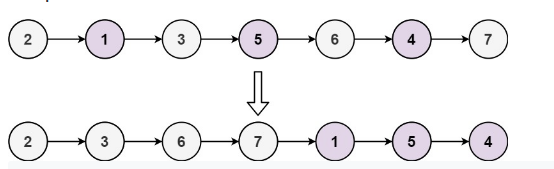
\includegraphics[scale=0.5]{images/oddEvenList.png}

\textbf{Entrada:} head = [2,1,3,5,6,4,7]

\textbf{Saída:} [2,3,6,7,1,5,4]


\begin{minted}{C++}

class ListNode {
    public:
    int val;
    ListNode *next;
    ListNode() : val(0), next(nullptr) {}
    ListNode(int x) : val(x), next(nullptr) {}
    ListNode(int x, ListNode *next) : val(x), next(next) {}

    
};


ListNode* oddEvenList(ListNode* head)
{
}
int main(){
    vector <int> v1({1,2,3,4,5});
    vector <int> v2({1,3,5,2,4});
    ListNode * head = toList(v1, 0, v1.size() - 1);
    head = oddEvenList(head);
    v1 = toVector(head);
    assert( v1 == v2 );
    return 0;    
}

\end{minted}


\item Dado o cabeça de uma lista encadeada simples ordenadas, exclua todas as duplicatas de forma que cada elemento apareça apenas uma vez. Retorne a lista encadeada ordenada também.

 
\textbf{Exemplo 1:}

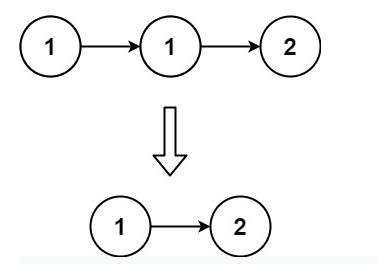
\includegraphics[scale=0.5]{images/deleteDuplicadas.png}


\textbf{Entrada:} head = [1,1,2]\\
\textbf{Saída:} [1,2]\\

\begin{minted}{C++}
class ListNode {
    public:
    int val;
    ListNode *next;
    ListNode() : val(0), next(nullptr) {}
    ListNode(int x) : val(x), next(nullptr) {}
    ListNode(int x, ListNode *next) : val(x), next(next) {}
};
ListNode* deleteDuplicates(ListNode* head) 
{
}
\end{minted}

\item Dados as cabeças de duas listas encadeadas, headA e headB, retorne o nó no qual as duas listas se cruzam. Se as duas listas encadeadas não tiverem nenhuma interseção, retorne nulo.

Por exemplo, as duas listas encadeadas a seguir começam a se cruzar no nó c1: 


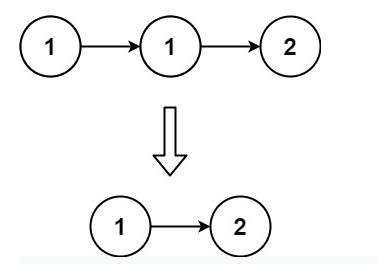
\includegraphics[scale=0.5]{images/deleteDuplicadas.png}

\textbf{Input:} headA = [4,1,8,4,5], headB = [5,6,1,8,4,5],

\textbf{Output:} list = [8,4,5]



\begin{minted}{C++}
class ListNode {
    public:
    int val;
    ListNode *next;
    ListNode() : val(0), next(nullptr) {}
    ListNode(int x) : val(x), next(nullptr) {}
    ListNode(int x, ListNode *next) : val(x), next(next) {}
};
ListNode *getIntersectionNode(ListNode *headA, ListNode *headB);
\end{minted}

\item Dada a cabeça de uma lista encadeada e um inteiro val, remova todos os nós da lista encadeada que possui Node.val == val e retorne a nova cabeça.

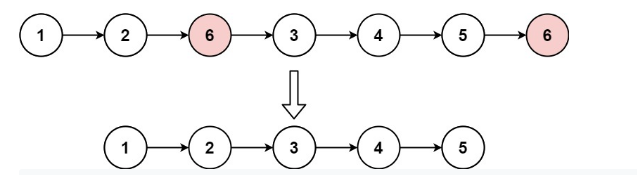
\includegraphics[scale=0.5]{images/removeElements.png}

Input: head = [1,2,6,3,4,5,6], val = 6

Output: [1,2,3,4,5]

\item Dado duas cabeças de duas listas encadeadas ordenadas, list1 e list2.

Mescle as duas listas em uma única lista ordenada. A lista deve ser feita juntando os primeiros nós das duas primeiras listas.

Retorne a cabeça da lista encadeada mesclada.

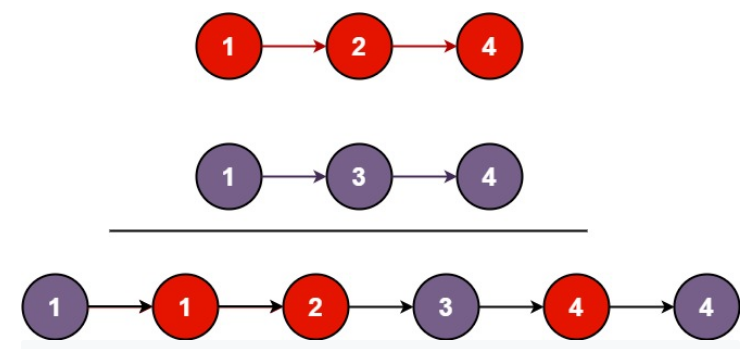
\includegraphics[scale=0.5]{images/mergelist.png}

Input: list1 = [1,2,4], list2 = [1,3,4]\\
Output: [1,1,2,3,4,4]\\

\item Dada a cabeça de uma lista encadeada simples, inverta a lista e retorne a lista invertida.

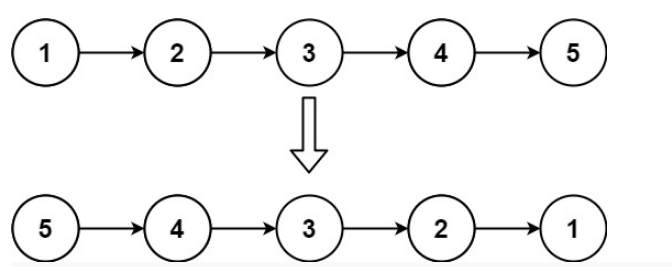
\includegraphics[scale=0.5]{images/reverseList.png}

Input: head = [1,2,3,4,5]\\
Output: [5,4,3,2,1]\\



\end{enumerate}


\section{Lista encadeada com descritores}

Um descritor de uma estrutura de dados é uma informação que ajuda a descrever a nossa estrutura e permite que algumas operações possam ser realizada de maneira mais eficiente.

A implementação da lista duplamente encadeada apresentada aqui possui os seguintes descritores:
\begin{itemize}
    \item Um nó sentinela chamado head que aponta para o primeiro elemento da nossa lista encadeada.
    \item Um nó sentinela chamado past\_last que é o próximo do último elemento da lista encadeada.
    \item a variável inteira count representando o tamanho da lista encadeada.
\end{itemize}

Observe que com esses descritores podemos facilmente adicionar um elemento no ínicio da lista encadeada e saber o tamanho da lista encadeada.

Além disso, temos duas classes aninhadas:

\begin{itemize}
    \item A classe Node que descreve o nó de uma lista encadeada.
    \item A classe Iterator utilizada para navegar pela lista encadeada sem expor sua representação interna.
\end{itemize}


\begin{listing}[!ht]
\caption{Definição da Lista encadeada simples com descritores}
\begin{minted}{C++}
template <typename T> 
class List{
    private:
        class Node;
        Node * head;
        Node * past_last;
        int count;
    public:        
        class Iterator;
        List() : count(0) { 
            head = new Node();
            past_last = new Node();
            head->next = past_last;
        }
        ~List(){   
        }    
        int size() { return count; }
        Iterator begin();
        Iterator before_begin();
        Iterator end();
        void pop_front();
        void insert_front(T val);
        T & front();
        void insert_after(Iterator it, T val); 
        void erase_after(Iterator it);
};
\end{minted}
\end{listing}

\begin{listing}[!ht]
\caption{Definição do nó de uma lista encadeada simples}
\begin{minted}{C++}
template <typename T>
class List<T>::Node{
    public:
    T val;
    Node * next;
    Node() : next(nullptr){}
    Node(T val, Node * ptr = nullptr) : val(val), next(ptr) {}
    
};
\end{minted}
\end{listing}

\begin{listing}[!ht]
\caption{Definição do iterador da lista encadeada simples}
\begin{minted}{C++}
template <typename T>
class List<T>::Iterator
{
    private:
    Node *atual;
    public:
    Iterator() : atual(nullptr){}
    
    Iterator(Node * atual) : atual(atual){ }
    
    Iterator next(){ return Iterator( atual->next); }
    
    T & value() { return atual->val; }
    
    bool operator!=(const Iterator & other) const{
        return atual != other.atual;
    }
    
    void insert_after(T val)
    {
        Node * ptr = new Node(val, atual->next);
        atual->next = ptr;
    }

    void erase_after()
    {
        Node * ptr = atual->next;
        atual->next = atual->next->next;
        delete ptr;
    }

};

\end{minted}
\end{listing}


\begin{listing}[!ht]
\caption{Definição dos métodos da lista encadeada simples}
\begin{minted}{C++}
template <typename T> 
T & List<T>::front()
{
    return head->next->val;
}
template <typename T> 
typename List<T>::Iterator List<T>::begin()
{
    return Iterator(head->next);
}
template <typename T> 
typename List<T>::Iterator List<T>::before_begin()
{
    return Iterator(head);
}
template <typename T> 
typename List<T>::Iterator List<T>::end()
{
    return Iterator(past_last);
}
template <typename T> 
void List<T>::pop_front(){
    if(count > 0){
        Node * ptr = head->next;
        head->next = head->next->next;
        count--;
        delete ptr;
    }
}
template <typename T> 
void List<T>::insert_front(T val)
{
    Node * ptr = new Node(val, head->next);
    head->next = ptr;
    count++;   
}
template <typename T> 
void List<T>::insert_after(Iterator it, T val)
{
    it.insert_after(val);
}
template <typename T> 
void List<T>::erase_after(Iterator it)
{
    it.erase_after();
}
\end{minted}
\end{listing}

% \section{STL List}

% Na STL do C++, temos dois tipos de listas:

% \begin{itemize}
%     \item forward\_list implementada como uma lista encadeada simples.
%     \item list implementada como uma lista duplamente encadeada.
% \end{itemize}

% \subsection{insertion\_sort}

% No código seguinte, comparamos insertion\_sort com a utilização de vector e list da STL.

% \begin{minted}{C++}
% #include <bits/stdc++.h>
% #include "debug.h"

% using namespace std;

% void insert(list <int> & l, int x){
%     auto it = l.begin();
%     for(; it != l.end(); ++it){
%         if(*it > x){
%             break;
%         } 
%     }
%     l.insert(it, x);
% }

% void insertion_sort(list <int> & l){
%     if(l.size() > 1){
%         int x = l.front();
%         l.pop_front();
%         insertion_sort(l);
%         insert(l, x);
%     }
% }

% void insert(vector<int> & v, int p, int r){
%     int x = v[p];
%     int j = p+1;
%     while( j <= r && v[j] < x){
%         v[j-1] = v[j];
%         j++;
%     }
%     v[j-1] = x;
% }


% void insertion_sort(vector <int> & v, int p,int r){    
%     if( r > p ){
%         int x = v[r];
%         insertion_sort(v, p+1, r);
%         insert(v, p, r);
%     }
% }


% vector <int> generate(int size, int limite_inferior = 0, int limite_superior = (int)1e9){
%     vector <int> output;
%     default_random_engine generator;
%     uniform_int_distribution<int> distribution(limite_inferior, limite_superior);

%     output.resize(size);
%     for(int i = 0; i < size; i++){
%         output[i] = distribution(generator);
%     }
%     return output;
% }



% int main(){

%     clock_t start, end;
%     vector <int> data = generate(10000, 0, 1000000);
    

%     list <int> l(data.begin(), data.end());
%     start = clock();
%     insertion_sort(l);
%     end = clock();
%     printf ("execution time %lf seconds.\n",((double) end-start)/CLOCKS_PER_SEC);
        
    
%     vector <int> A(data.begin(), data.end());
%     start = clock();
%     insertion_sort(A, 0 , A.size() - 1);
%     end = clock();
%     printf ("execution time %lf seconds.\n",((double) end-start)/CLOCKS_PER_SEC);    
% }

% //execution time 0.272482 seconds.
% //execution time 0.106265 seconds.


% \end{minted}

% Note que mesmo que com o tempo constante para a inserção e remoção da list da STL. O tempo de execução não é reduzido.


% \subsection{Josephus Problem}

% Nesta seção, vamos comparar três soluções para o problema Josephus:

% \begin{itemize}
%     \item JosephusArray: utiliza um array auxiliar para guardar as pessoas vivas, a operação de matar é realizada em tempo constante e a operação de buscar o próximo vivo é realizada em tempo linear.
%     \item JosephusVector: utiliza stl vector, a operação de matar é realizada em tempo linear e a operação de buscar o próximo vivo é realizada em tempo linear.
%     \item JosephusList: utiliza stl list, a operação de matar é realizada em tempo constante e a operação de buscar o próximo vivo é realizada em tempo constante.
% \end{itemize}


% \begin{center}
% \begin{tabular}{ccc}
% Implementação & matar & buscar o próximo vivo\\
% \hline 
% JosephusArray & $\mathcal{O}(1)$ & $\mathcal{O}(n)$\\
% JosephusVector & $\mathcal{O}(n)$ & $\mathcal{O}(1)$\\
% JosephusList & $\mathcal{O}(1)$ & $\mathcal{O}(1)$\\
% \end{tabular}
% \end{center}



% \begin{minted}{C++}

% #include <iostream>
% #include <bits/stdc++.h>
% using namespace std;

% int JosephusArray(int n, int k)
% {
%     k--;
%     int arr[n];
%     for (int i = 0; i < n; i++) {
%         arr[i] = 1; 
%     }
%     int cnt = 0, cut = 0, num = 1; // Cut = 0 gives the sword to 1st person.
%     while (cnt < (n - 1)) // Loop continues till n-1 person dies.
%     {
%         while (num <= k) // Checks next (kth) alive persons.
%         {
%             cut++;
%             cut = cut % n; // Checks and resolves overflow
%                           // of Index.
%             if (arr[cut] == 1) {
%                 num++; // Updates the number of persons
%                       // alive.
%             }
%         }
%         num = 1; // refreshes value to 1 for next use.
%         arr[cut] = 0; // Kills the person at position of 'cut'
%         if(num%100000==0)
%             printf("person %d died %d\n", num, cut );
%         cnt++; // Updates the no. of killed persons.
%         cut++;
%         cut = cut % n; // Checks and resolves overflow of Index.
%         while (arr[cut] == 0) // Checks the next alive person the
%                      // sword is to be given.
%         {
%             cut++;
%             cut = cut % n; // Checks and resolves overflow
%                           // of Index.
%         }
%     }
%     return cut + 1; // Output is the position of the last
%                     // man alive(Index + 1);
% }

% int JosephusVector(int n, int k){
%     vector <int> v;
%     for(int i = 0; i < n; i++)
%     {
%         v.push_back(i+1);
%     }

%     auto it = v.begin();

%     while(v.size()>1)
%     {
%         for(int i=1;i<k;i++)
%         {
%             it++;  
%             if(it==v.end()) it = v.begin();
%         }

%         it = v.erase(it);
          
%         if(it==v.end())
%         {
%             it = v.begin();
%         }
%     }
     
%     return v[0]; //returns front element of the list//
    



% }


% int JosephusList(int n, int k){
%     list<int>l; //creates a doubly linked list using stl container//
%     for(int i=0;i<n;i++)
%         l.push_back(i+1); //pushes i to the end of the doubly linked list//
      
%     auto it = l.begin(); 
%     while(l.size()>1){
         
%         for(int i=1;i<k;i++){
%             it++;
             
%             if(it==l.end()){
%               //if iterator reaches the end,then we change it to begin of the list//
%                 it = l.begin();
%             }
%         }

%         int num = n -l.size() + 1;    
%         if(num %100000 == 0)  
%         printf("person %d died %d\n", num , *it);

%          it = l.erase(it);
          
%          if(it==l.end()){
%           //if iterator reaches the end,then we change it to begin of the list//
%                 it = l.begin();
%             }
%     }
     
%     return l.front(); //returns front element of the list//
     
% }

% int main(){

%     int n = 1e5, k = 1e4, x;
%     clock_t start, end;

%     start = clock();
%     x = JosephusArray(n, k);
%     end = clock();
%     printf("sobrevivente %d\n", x);
%     printf("execution time %lf seconds.\n",((double) end-start)/CLOCKS_PER_SEC);

%     start = clock();
%     x = JosephusList(n, k);
%     end = clock();
%     printf("sobrevivente %d\n", x);
%     printf("execution time %lf seconds.\n",((double) end-start)/CLOCKS_PER_SEC);

%     start = clock();
%     x = JosephusVector(n, k);
%     end = clock();
%     printf("sobrevivente %d\n", x);
%     printf("execution time %lf seconds.\n",((double) end-start)/CLOCKS_PER_SEC);


%     return 0;

% }

% /*
% sobrevivente 45338
% execution time 41.915037 seconds.
% sobrevivente 45338
% execution time 7.246956 seconds.
% sobrevivente 45338
% execution time 9.671076 seconds.
% */
% \end{minted}





\chapter{Listas duplamente encadeadas}

No capítulo anterior, vimos que a lista encadeada simples é uma estrutura recursiva que contém pelo menos dois campos: um valor (val) e um ponteiro para o próximo nó. As listas encadeadas simples permitem a construção de lista com tamanho dinâmico sem acesso randômico. Essa estrutura permite um gerenciamento de memória mais flexível. Além disso, elas permitem que as operações de inserção e deleção possam ser feita em tempo constante. 


\begin{center}
\begin{tabular}{|l|ll|}
\hline
\multicolumn{1}{|c|}{\multirow{2}{*}{Estrutura de Dados}} & \multicolumn{2}{l|}{Inserção e deleção} \\ \cline{2-3} 
\multicolumn{1}{|c|}{}                                    & \multicolumn{1}{l|}{Início}    & Fim    \\ \hline
Lista Sequencial Dinâmica                                 & \multicolumn{1}{l|}{O(n)}      & O(1)   \\ \hline
Lista encadeada simples com nó cabeça                     & \multicolumn{1}{l|}{O(1)}      & O(n)   \\ \hline
Lista encadeada simples com nó cabeça e nó rabo           & \multicolumn{1}{l|}{O(1)}      & O(1)   \\ \hline
\end{tabular}
\end{center}

A principal desvantagem das listas encadeadas é permitir apenas a travessia em apenas uma direção. Além disso, só podemos inserir um novo elemento após um dado nó. Essa restrição pode tornar alguns problemas mais complicados.



Considere a seguinte definição do nó de uma lista encadeada simples:
\begin{listing}[!ht]
\caption{Definição do nó de uma lista encadeada simples}

\begin{minted}{C++}
template <typename T>
class Node {
    public:
    T val;
    Node *next;
    Node() : val( T() ), next(nullptr) {}
    Node(T x) : val(x), next(nullptr) {}
    Node(T x, Node *next) : val(x), next(next) {} 
};

\end{minted}
\end{listing}


Considere que você recebe o ponteiro para nó cabeça de uma lista encadeada simples e um nó da lista a ser removido. Para remover esse nó da lista precisamos encontrar o nó anterior a ele para que esse nó aponte para o próximo do nó removido.

\newpage 
\begin{listing}[!ht]
\caption{Deleção de um nó em uma lista encadeada simples}

\begin{minted}{C++}

template <typename T>
Node<T> * deleteNode(Node<T> * head, Node<T> * node){
    if(head == nullptr )
        return head;
    else if(head == node){
        auto ptr = head->next;
        delete head;
        return ptr;
    }else{
        auto prev = head;
        while( prev->next != node){
            prev = prev->next;
        }
        prev->next = node->next;
        delete node;
        return head;
    }
}
\end{minted}
\end{listing}

Considere agora a  seguinte definição de uma lista encadeada duplamente encadeada:


\begin{listing}[!ht]
\caption{Definição do nó de uma lista duplamente encadeada}
\begin{minted}{C++}
template <typename T>
class Node {
    public:
    T val;
    Node *next;
    Node *prev;
    Node() : val( T()  ), next(nullptr), prev(nullptr) {}
    Node(T x) : val(x), next(nullptr), prev(nullptr) {}
    Node(T x, Node *prev, Node *next) : val(x), prev(prev), next(next) {} 
};

\end{minted}
\end{listing}

O mesmo problema pode ser resolvido facilmente na lista duplamente encadeada. Como pode ser visto na Listagem \ref{listing::DeleteNodeDouble}.

\begin{listing}[!ht]
\caption{Deleção de um nó uma lista duplamente encadeada}
\label{listing::DeleteNodeDouble}
\begin{minted}{C++}
template <typename T>
Node<T> * deleteNode(Node<T> * head, Node<T> * node)
{
    node->prev->next = node->next;
    node->next->prev = node->prev;
    delete node;

    return head;
}
\end{minted}
\end{listing}



\section{Recursão em listas duplamente encadeada}

\subsection{Busca de um elemento}
Dado o nó cabeça de uma lista duplamente encadeada. Sua tarefa é
verificar se um elemento x está presente na lista duplamente encadeada.

Matematicamente, podemos expressar esse problema recursivamente da seguinte maneira:


\begin{equation}
search(head, x) = 
\begin{cases}
false           & , head == nullptr\\
true            & , head->val == x\\
search(head->next, x) & , \text{caso contrário}\\

\end{cases}
\end{equation}

\textbf{Caso Base}

Neste problema, temos dois casos bases:

\begin{enumerate}
    \item Quando a lista duplamente encadeada está vazia (head == nullptr). Neste caso, devolvemos o valor booleano falso.
    \item Quando o valor armazenado na cabeça da lista é igual ao valor x buscado (head->val == x). Neste caso, devolvemos o valor booleano true. 
\end{enumerate}


\textbf{Caso Recursivo}

Neste caso, podemos reduzir o problema para um caso menor, ou seja, buscar o elemento x na lista duplamente encadeada cuja cabeça é head->next.


\begin{listing}[!ht]
\caption{Busca de um elemento em uma lista duplamente encadeada}
\label{listing::DeleteNodeDouble}
\begin{minted}{C++}
template <typename T>
bool * searchNode(Node<T> * head, T x)
{
    if(head == nullptr)
        return false;
    else if(head->val == x)
        return true;
    else   
        return searchNode(head->next, x);
}
\end{minted}
\end{listing}


\subsection{Remover um elemento de uma lista encadeada}

Dado o nó cabeça de uma lista duplamente encadeada. Sua tarefa é
remover o nó com o valor x da lista duplamente encadeada.

Matematicamente, podemos expressar esse problema recursivamente da seguinte maneira:


\begin{equation}
remove\_element(head, x) = 
\begin{cases}
head            & , head == nullptr\\
head->next      & , head->val == x\\
ptr = remove\_element(head->next, x) & , \text{caso contrário}\\
head->next = ptr & , \text{caso contrário}\\
ptr->prev = head & , \text{caso contrário}\\
\end{cases}
\end{equation}

\textbf{Caso Base}

Neste problema, temos dois casos bases:

\begin{enumerate}
    \item Quando a lista duplamente encadeada está vazia (head == nullptr). Neste caso, devolvemos nullptr.
    \item Quando o valor armazenado na cabeça da lista é igual ao valor a ser removido. Neste caso, devolvemos head->next.  
\end{enumerate}

\textbf{Caso Recursivo}

Quando o valor armazenado na cabeça da lista é diferente ao valor a ser removido, reduziremos o problema a remove o elemento x da lista duplamente encadeada com a cabeça em head->next com resultado ptr. Em seguida, reconstruiremos a lista duplamente encadeada inicial com as seguintes operações:

\begin{enumerate}
    \item head->next = ptr
    \item ptr->prev  = head, se ptr != nullptr
\end{enumerate}

\begin{listing}[!ht]
\caption{Remover um elemento de uma lista duplamente encadeada}
\begin{minted}{C++}
template <typename T>
Node<T> * remove_element(Node<T> * head, T x){
    if(head == nullptr)
        return nullptr;
    else
    {
        if(head->val == x)
        {
           auto ptr  = head->next;
           delete head;
           return ptr;
        }
        else
        {
            head->next = remove_element(head->next, x);
            if( head->next )
                head->next->prev = head;
            return head;
        }
    }
}
\end{minted}
\end{listing}

\section{Lista Duplamente Encadeada com descritores}

Um descritor de uma estrutura de dados é uma informação que ajuda a descrever a nossa estrutura e permite que algumas operações possam ser realizada de maneira mais eficiente.

A implementação da lista duplamente encadeada apresentada aqui possui os seguintes descritores:
\begin{itemize}
    \item Um nó sentinela chamado head que aponta para o primeiro elemento da nossa lista encadeada.
    \item Um nó sentinela chamado past\_last que é o próximo do último elemento da lista encadeada.
    \item a variável inteira count representando o tamanho da lista encadeada.
\end{itemize}

Observe que com esses descritores podemos facilmente adicionar um elemento no ínicio e fim da lista encadeada e saber o tamanho da lista encadeada.

Além disso, temos duas classes aninhadas:

\begin{itemize}
    \item A classe Node que descreve o nó de uma lista encadeada.
    \item A classe Iterator utilizada para navegar pela lista encadeada sem expor sua representação interna.
\end{itemize}



\begin{listing}[!ht]
\caption{Definição da Lista duplamente encadeada com descritores}
\begin{minted}{C++}
template <typename T> 
class List;

template <typename T> 
class List{
    private:
        class Node;
        Node * head;
        Node * past_last;
        int count;
    public:        
        class Iterator;
        List();
        int size();
        void insert_front(T x);
        void insert_back(T x);
        void remove_front();
        void remove_back();
        T & front();
        T & back();
        auto begin();
        auto end();
        void insert_before(Iterator it, T x);
        void erase_before(Iterator it);
};
\end{minted}
\end{listing}


\begin{listing}[!ht]
\caption{Definição do nó de uma lista duplamente encadeada}
\begin{minted}{C++}
template <typename T> 
class List<T>::Node{
    public:
    T val;
    Node * next;
    Node * prev;
    Node() : next(nullptr), prev(nullptr){}
    Node(T val) : next(nullptr), prev(nullptr){}
    Node(T val, Node * prev, Node * next) : val(val), prev(prev), next(next) {}    
};


\end{minted}
\end{listing}



\begin{listing}[!ht]
\caption{Definição do iterador da lista duplamente encadeada}
\begin{minted}{C++}
template <typename T> 
class List<T>::Iterator{
    private:
        Node *atual;
    public:
        Iterator() : atual(nullptr){}
        Iterator(Node * atual) : atual(atual){ }
        Iterator next(){ return Iterator( atual->next); }
        T & value() { return atual->val; }
        bool operator!=(const Iterator & other) const{
            return atual != other.atual;
        }
        void insert_before(T x)
        {
            auto ptr = new Node(x, atual->prev, atual);
            atual->prev->next = ptr;
            atual->prev = ptr;
        }
        void erase_before()
        {
            auto ptr = atual->prev;

            ptr->prev->next = atual;
            atual->prev = ptr->prev;

            delete ptr;

        }
};
\end{minted}
\end{listing}



\begin{listing}[!ht]
\caption{Definição de algumas operações da lista encadeada}
\begin{minted}{C++}
template <typename T> 
void List<T>::remove_front(){
    if(count > 0){
        auto ptr = head->next;
        head->next = ptr->next;
        ptr->next->prev = head;
        delete ptr;
        this->count--;
    }
}
template <typename T> 
void List<T>::remove_back(){
    
    if(count > 0){
        auto last = past_last->prev;
        past_last->prev = last->prev;
        last->prev->next = past_last;
        delete last;
        this->count--;
    }
}
template <typename T> 
void List<T>::insert_front(T x){
    auto ptr = new Node(x, head, head->next);
    head->next->prev = ptr;
    head->next = ptr;
    this->count++;
}
template <typename T> 
void List<T>::insert_back(T x){
    auto ptr = new Node(x, past_last->prev, past_last);
    past_last->prev->next = ptr;
    past_last->prev = ptr;
    this->count++;
}

\end{minted}
\end{listing}



\chapter{Pilha}

A pilha é uma estrutura de dados que manipula uma coleção de elementos com duas operações principais:

\begin{itemize}
\item push: que adiciona um elemento na coleção.
\item pop: que remove o elemento que ainda não foi removido adicionado mais recentemente.
\end{itemize}

%Na pilha, a ordem em que os elementos saem da pilha é conhecida pelo acrônimo LIFO (Last in, First out). 

A ideia da estrutura de dados pilha começou a aparecer na literatura da ciência da computação em 1946 com Alan Turing no relatório com o título Propostas para Desenvolvimento na Divisão de Matemática de uma Máquina Automática de Computação\footnote{ \url{https://academic.oup.com/comjnl/article-pdf/20/3/269/2256995/200269.pdf}}.
Ele usou os termos enterrar (bury) and desenterrar (unbury) para o gerenciamento das subrotinas. Em 1957, Klaus Samuelson e Friedrich L. Bauer depositaram uma patente com a idéia da pilha. 



Frequentemente, as pilhas são apresentadas como uma pilha de pratos onde os pratos limpos são colocados no topo da pilha. Note que na pilha de pratos, os primeiros pratos que saem da pilha são os últimos que foram empilhados. Essa política de gerenciamento é conhecida como LIFO (Last in, First out).

As pilhas com tamanho dinâmico podem ser implementadas utilizado as listas sequencias com tamanho dinâmico ou listas encadeadas. 

Na linguagem C++, a classe stack suporta as seguintes operações:

\begin{itemize}
\item empty
\item pop
\item push
\item size
\item top
\end{itemize}


Em alguns casos, podemos implementar a classe stack como uma classe derivada diretamente da classe vector.

\begin{minted}{C++}
template <typename T> 
class stack : public std::vector <T>
{
  public:
  using base_type = std::vector <T> ;
  void  push ( const T& x ) { base_type::push_back( x ); }
  const T& top  ()             { return base_type::back(); }
  void  pop  ()             { base_type::pop_back(); }
  bool  empty()             { return base_type::empty(); }
};
\end{minted}

Podemos implementar a classe stack utilizando um vector internamente.

\begin{minted}{C++}
template <typename T> 
class stack 
{
  using base_type = std::vector <T> ;
  private:
    base_type data;
  public:
  void  push ( const T& x ) { data.push_back( x ); }
  const T& top  ()             { return data.back(); }
  void  pop  ()             {  data.pop_back(); }
  bool  empty()             { return data.empty(); }
};
\end{minted}

\section{Recursão}

As linguagens de programação que suportam recursão utilizam uma pilha de chamada (\textit{call stack}). Para cada chamada de um subprograma, um registro de ativação é criado na pilha de chamadas. No registro de ativação armazenamos algumas informações sobre o subprograma como:

\begin{itemize}
\item parâmetros
\item endereço de retorno
\item valor das variáveis locais 
\end{itemize}

Quando o subprograma não está mais ativo, essas informações deixam de ser armazenadas. 

Considere o seguinte programa recursivo:

\begin{minted}{C++}
int fact(int n){
    if(n==1)
        return 1;
    else
        return n*fact(n-1);
}
\end{minted}

A Figura abaixo mostra de maneira simplificada como a pilha de ativação é alterada para o cálculo de fact(3). 

\begin{figure}[htbp]
\centering
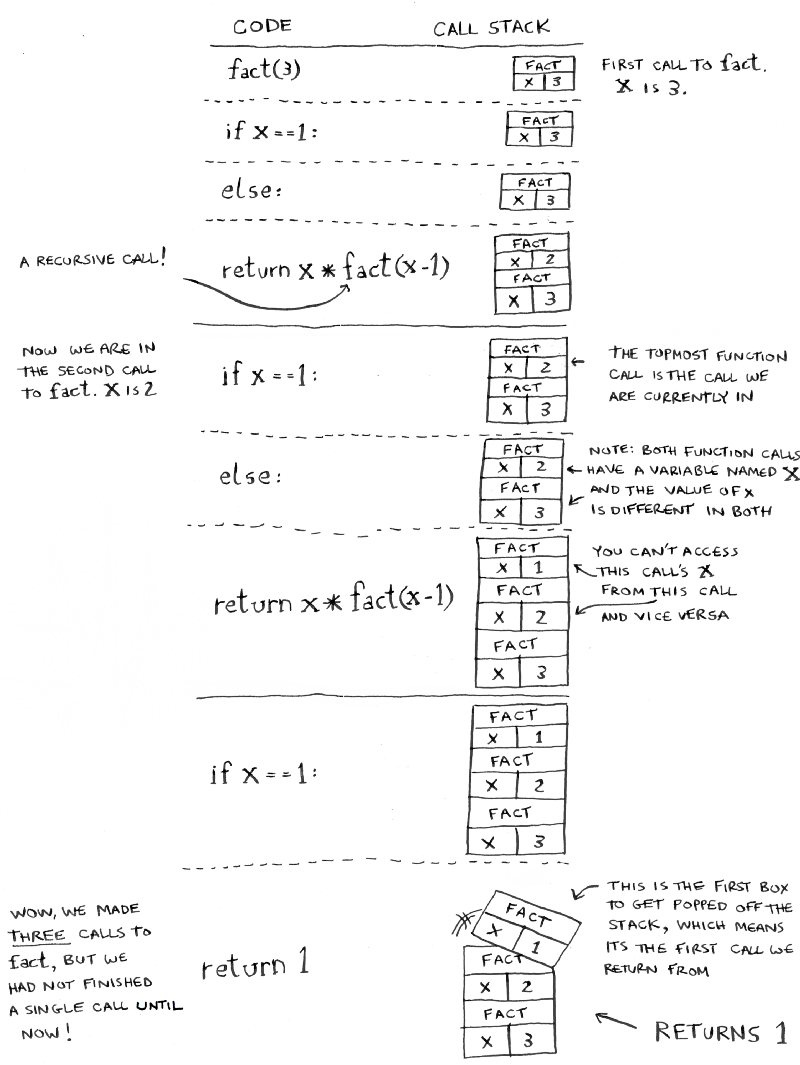
\includegraphics[scale=0.4]{images/callstack.png}
\caption{Image credit: Adit Bhargava} 
\end{figure}

\newpage 


O site Pythontutor permite também visualizar a pilha de chamadas de maneira simplificada.

\begin{figure}[htbp]
\centering
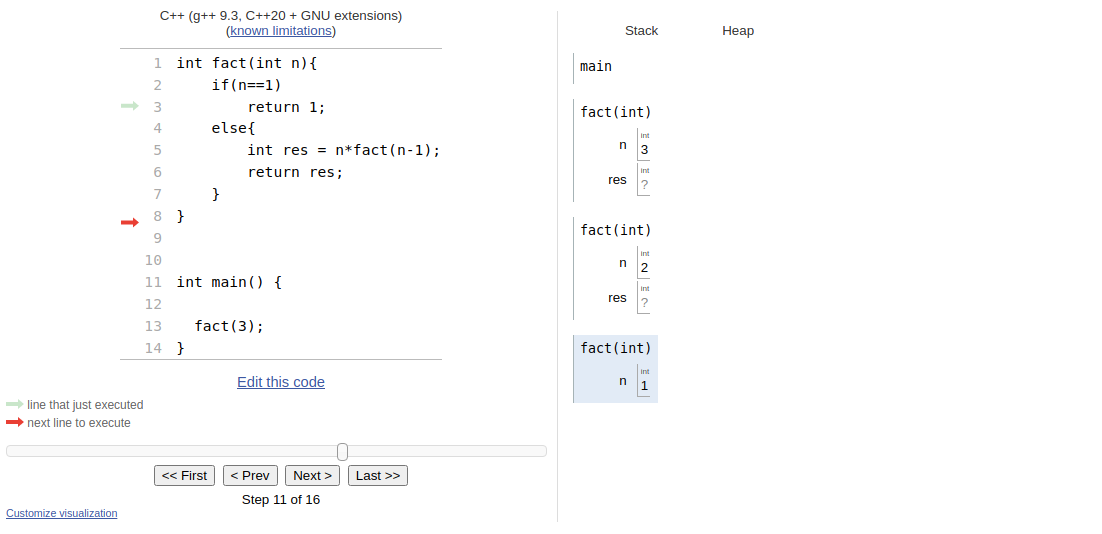
\includegraphics[scale=0.5]{images/pythontutor.png}
\caption{site pythontutor.com}
\end{figure}


Todo programa recursivo pode ser simulado utilizando uma pilha. Por exemplo, o programa fatorial pode ser simulado utilizando pilha da seguinte maneira:

\begin{minted}{C++}
int fact(int n){
    stack <int> s;
    while(n>1){
        s.push(n);
        n--;
    }
    int ret = 1; // caso base
    while( !s.empty() ){
        int u = s.top();
        ret = u*ret;
        s.pop();
    }
    return ret;
}
\end{minted}

No código seguinte, vamos simular o fatorial utilizando uma pilha de funções. Vamos empilhas as funções $n*,(n-1)*, \ldots ,2*$. Em seguida, vamos plugando o resultado obtido pela função desempilhada.

\begin{minted}{C++}

auto f(int a){
    return [=](int b){ return a*b; };
}
stack <  function<int(int)> > s;
void push(int n){
    while(n > 1){
        s.push(f(n)); // push n*
        n--;
    }
}
int calc_fact(int n){
    push(n);
    
    /*
    stacking
    2*
    .
    .
    .
    n-2*
    n-1*
    n*
    */

    int ret = 1;
    while( !s.empty() ){
        auto g = s.top();
        ret = g(ret); 
        s.pop();
    }
    return ret;
}
\end{minted}

\section{Fibonacci}

Considere o programa recursivo para o número de fibonacci:

\begin{minted}{C++}
int fibonacci(int n){
    if(n==1 || n == 2) return n;
    else return fibonacci(n-1) + fibonacci(n-2);
}
\end{minted}

Dessa vez, vamos simular o programa recursivo com duas pilhas. Uma pilha de operações que devem ser realizadas e uma pilha de valores de retorno.

\begin{minted}{C++}
enum class optype { sum, calc };
class Operation{
    public:
    optype op;
    int n;
    Operation(optype t, int v = 0): op(t), n(v) {} 
};

int calc_fibonacci(int n){
    stack <Operation> s;
    stack <int> ret;
    s.push( Operation(optype::calc, n) );
    while( !s.empty() ){
        auto u = s.top();
        s.pop();
        if( u.op == optype:: calc )
        {
            if( u.n == 1 || u.n == 2 ){
                ret.push(u.n);
            }else{
                s.push( Operation( optype::sum )      );
                cout << "pushing sum" << endl;
                s.push( Operation( optype::calc, u.n-1) );
                cout << "pushing calc " << u.n-1 << endl;
                s.push( Operation( optype::calc, u.n-2) );
                cout << "pushing calc " << u.n-2 << endl;   
            }
        } 
        else if( u.op == optype:: sum )
        {         
            int a,b;
            a = ret.top();
            ret.pop();
            cout << "popping " << a << endl;
            b = ret.top();
            cout << "popping " << b << endl;
            ret.pop();
            ret.push(a+b);
            cout << "pushing " << a+b << endl;
            
        }
        
    }
    return ret.top();
}
\end{minted}

No cálculo do fibonacci(6), temos o programa escreve as seguintes mensagens:

\begin{minted}{C++}
pushing sum
pushing calc 5
pushing calc 4
pushing sum
pushing calc 3
pushing calc 2
pushing sum
pushing calc 2
pushing calc 1
popping 2
popping 1
pushing 3
popping 3
popping 2
pushing 5
pushing sum
pushing calc 4
pushing calc 3
pushing sum
pushing calc 2
pushing calc 1
popping 2
popping 1
pushing 3
pushing sum
pushing calc 3
pushing calc 2
pushing sum
pushing calc 2
pushing calc 1
popping 2
popping 1
pushing 3
popping 3
popping 2
pushing 5
popping 5
popping 3
pushing 8
popping 8
popping 5
pushing 13


\end{minted}




\section{Algoritmo Shunting Yard}

O algoritmo Shunting Yard foi proposto por Edsger Dijkstra em 1961 para converter uma expressão infixa em uma expressão na notação polonesa reversa usando pilha. 

A notação polonesa foi proposta pelo lógico polonês Jan Łukasiewicz em 1924. Nessa notação, os operadores aparecem antes dos seus operandos.

Já a notação polonesa reversa foi proposta em 1954 por Arthur Burks, Don Warren e Jesse Wright e de maneira independente em 1961 por Friedrich L. Bauer e Edsger W. Dijkstra para auxiliar no processo de avaliação de expressões nas linguagens de programação.


Na notação polonesa reversa, primeiramente escrevemos os operandos em seguida os operadores. A notação polonesa reversa possui duas vantagens principais:

\begin{enumerate}
\item A expressão não precisa utilizar os parênteses uma vez que cada operador tem um número fixo de operandos.
\item As regras de associatividade e precedência não precisam ser definidas.
\end{enumerate}

Por exemplo, a expressão A + B * C fica A B C * +.

O processo de conversão da expressão infixa para a expressão na notação polonesa reversa pode ser realizada pela seguintes regras.

\begin{enumerate}
\item Se o símbolos da entrada forem um operando, imprima-o.

\item Se o símbolo da entrada for um parêntese esquerdo, empilhe-o na pilha.

\item Se o símbolo da entrada for um parêntese direito: descarte o parêntese direito, desempilhe e imprima os símbolos da pilha até ver um parêntese esquerdo. Desempilhe o parêntese esquerdo e descarte-o.

\item Se o símbolo da entrada for um operador e a pilha estiver vazia ou contiver um parêntese esquerdo no topo, empilhe o operador da entrada para a pilha.

\item Se o símbolo da entrada for um operador e tiver precedência mais alta do que o operador no topo da pilha, ou tiver a mesma precedência do operador no topo da pilha e for associativo à direita - empilhe-o na pilha.

\item Se o símbolo da entrada for um operador e tiver precedência inferior ao operador no topo da pilha, ou tiver a mesma precedência do operador no topo da pilha e for associativo à esquerda - continue a desempilhar da pilha até que seja verdade. Em seguida, empilhe o operador de entrada.

\item No final da expressão, desempilhe e imprima todos os operadores na pilha. (Nenhum parêntese deve permanecer.)

\end{enumerate}

Nos exemplos seguintes utilizaremos, o símbolo \$ para representar o final da expressão.

\begin{exemplo}
Considere o processo de conversão da seguinte expressão A + B * C\$.

\begin{tabular}{llll}
  &Símbolo da Entrada    & Pilha  & Notação Polonesa Reversa \\
1 & A     &    & A \\
2 & +     & +  & A \\
3 & B     & +  & A B\\
4 & *     & + *  & A B\\
5 & C     & + *  & A B C\\
6 & \$     &    & A B C * +\\

\end{tabular}


\end{exemplo}


\begin{exemplo}
Considere o processo de conversão da seguinte expressão A * (B + C * D) + E\$.

\begin{tabular}{llll}
  &Símbolo da Entrada    & Pilha  & Notação Polonesa Reversa \\
1 & A     &    & A \\
2 & *     & *  & A \\
3 & (     & * ( & A \\
4 & B     & * (  & A B\\
5 & +     & * ( +  & A B\\
6 & C     & * ( +   & A B C\\
7 & *     & * ( + *   & A B C\\
8 & D     & * ( + *   & A B C D\\
9 & )     & *    & A B C D * + *\\
10 & +    & +    & A B C D * + * \\
11 & E    & +    & A B C D * + * E\\ 
12 & \$   &     & A B C D * + * E +\\ 

\end{tabular}


\end{exemplo}


\textbf{Exercício:}

\begin{enumerate}
    \item Dado uma expressão na notação polonesa reversa com os operadores +,-,*,/ calcule o valor da expressão utilizando uma pilha.
\end{enumerate}




\section{Stack-Insertion Sort}

O algoritmo Stack-Insertion Sort pode ser implementado utilizando duas pilhas chamadas esquerda e direita. A pilha esquerda é usada para empilhar os itens em ordem crescente, enquanto a pilha da direita é usada para empilhar os elementos em ordem decrescente. O topo de cada pilha no passo i representa o ponto de inserção do elemento i. A pilha da esquerda começa empilhando o menor valor ($-\infty$) e pilha direita começa empilhando o maior valor ($+ \infty$).  


O algoritmo Stack-Insert Sort pode ser implementado da seguinte maneira:

\begin{algorithm}
\caption{Stack-Insert Sort}
\begin{algorithmic}

\State $i \gets 1$
\State esquerda.push($-\infty$)
\State direita.push($+\infty$)

\While{ $i \leq n$}
    
    \If{$a_i$ $<$ esquerda.top()}
    \While{ $a_i < $ esquerda.top()}
    \State direita.push(esquerda.top())
    \State esquerda.pop()
    \EndWhile
    \State esquerda.push($a_i$)
    \Else
        \If{$a_i$ $<$ direita.top()}
        \State direita.push($a_i$)
        \Else
            \While{ $a_i > $ direita.top()}
            \State esquerda.push(direita.top())
            \State direita.pop()
            \EndWhile
            \State direita.push($a_i$)
        \EndIf
    \EndIf
    
    
    \State $i \gets i + 1$
    
\EndWhile

\While { direita.top() $\neq +\infty$ }
\State esquerda.push(direita.top())
\State direita.pop()
\EndWhile 
\end{algorithmic}
\end{algorithm}

\begin{exemplo}
Execução do algoritmo Stack-Insert Sort para o vetor a = [20,67,07,31,53,11,6,55]

\begin{tabular}{lll}
\hline
         & a        &   20 67 07 31 53 11 6 55        \\
passo 0  &   esquerda & $-\infty$                                \\
         & direita  & $+\infty$\\
\hline
         & a        &   67 07 31 53 11 6 55        \\
passo 1  &   esquerda & $-\infty$                                \\
         & direita  & $+\infty$ 20\\
\hline
         & a        &   07 31 53 11 6 55        \\
passo 2  &   esquerda & $-\infty$ 20                               \\
         & direita  & $+\infty$ 67\\
\hline
         & a        &   31 53 11 6 55        \\
passo 3  &   esquerda & $-\infty$ 07                                \\
         & direita  & $+\infty$ 67 20\\
\hline
         & a        &   53 11 6 55        \\
passo 4  &   esquerda & $-\infty$ 07 20                               \\
         & direita  & $+\infty$ 67 31\\
\hline
         & a        &   11 6 55        \\
passo 5  &   esquerda & $-\infty$ 07 20 31                               \\
         & direita  & $+\infty$ 67 53\\
\hline
         & a        &   6 55        \\
passo 6  &   esquerda & $-\infty$ 07 11                                \\
         & direita  & $+\infty$ 67 53 31 20 \\
\hline
         & a        &   55        \\
passo 7  &   esquerda & $-\infty$ 06                                \\
         & direita  & $+\infty$ 67 53 31 20 11 07\\
\hline
         & a        &   -        \\
passo 8  &   esquerda & $-\infty$ 06 07 11 20 31 53                                 \\
         & direita  & $+\infty$ 67 55\\
\hline
         & a        &   -        \\
passo 9  &   esquerda & $-\infty$ 06 07 11 20 31 53 55 67                                 \\
         & direita  & $+\infty$ \\
\hline

\end{tabular}
\end{exemplo}

\chapter{Fila}

Na ciência da computação, uma fila é um estrutura de dados que mantém uma coleção de elementos de maneira que a operação de dequeue remove o elemento mais antigo da fila e operação enqueue adiciona um novo elemento na fila preservando a ordem de tempo na fila. Uma maneira fácil de implementar é manter descritores para o ínicio e o fim da fila. Esses descritores serão importantes para manter a corretude das operações enqueue e dequeue.

Na linguagem C++, a fila pode ser implementada estendendo a classe list (que por sua vez são implementadas como listas duplamente encadeadas) implementando as operações push\_back, pop\_front, front.

\begin{minted}{C++}
template <typename T> 
class queue : private list <T>
{
  public:
    using base_type = list <T> ; 
  void  enqueue ( const T& x ) { base_type::push_back( x ); }
  const T& front  ()             { return base_type::front(); }
  void  dequeue  ()             {  base_type::pop_front(); }
  bool  empty()             { return base_type::empty(); }
};
\end{minted}

Uma desvantagem de implementar a fila herdando da STL list é que a STL list é implementada como uma lista duplamente encadeada. Podemos implementar a fila usando uma lista encadeada simples guardando um ponteiro para o primeiro e o último elemento da lista. Na seção \ref{sec::queue_single_linked_list}, apresentamos a implementação da fila usando uma lista encadeada simples.


De igual modo, a fila também pode ser implementada estendendo a classe vector da linguagem C++. 

\begin{minted}{C++}

template <typename T> 
class queue : private vector <T>
{
  public:
    using base_type = vector <T> ; 
  void  enqueue ( const T& x ) { base_type::push_back( x ); }
  const T& front  ()             { return base_type::front(); }
  void  dequeue  ()             {  base_type::erase( base_type::begin() ); }
  bool  empty()             { return base_type::empty(); }
};

\end{minted}

Contudo, nessa implementação, a operação dequeue passa a ter complexidade linear. Lembrando que no vector a operação remove o primeiro elemento do vetor possui complexidade linear. Na seção \ref{sec::circular_ queue}, apresentamos uma implementação de uma fila circular utilizando um vetor de tamanho fixo em que a operação dequeue é realizada em tempo constante.









\section{Fila com lista encadeada simples com dois descritores}
\label{sec::queue_single_linked_list}

Nessa implementação, iremos implementar a fila utilizando dois ponteiros para o primeiro elemento e para o último. Na classe Node, teremos apenas um ponteiro para o próximo. Lembrando que na fila não temos uma travessia bidirecional.

\begin{minted}{C++}
template <typename T> 
class queue{
    private:
        class Node;
        Node * first;
        Node * last;
        int cnt;
    public:
        queue();
        ~queue();
        bool empty();
        void enqueue(T key);
        void dequeue();
        T front();
        int size();
};

template <typename T> 
class queue<T>::Node{
    public:
    T key;
    Node * next; 
    Node(T key, Node * next = nullptr) : key(key), next(next) {};
};
\end{minted}


As operações da lista podem ser implementadas facilmente:

\begin{minted}{C++}
template <typename T> 
queue<T>::queue()
{
    first = last = nullptr;
    cnt  = 0;
}
template <typename T> 
queue<T>::~queue(){
    auto ptr = first;
    while(ptr){
        auto temp = ptr;
        ptr = ptr->next;
        delete temp;
    }
    first = last = nullptr;
    cnt = 0;
}

template <typename T> 
bool queue<T>::empty()
{
    return cnt == 0;
}

template <typename T> 
int queue<T>::size()
{
    return cnt;
}

template <typename T> 
void queue<T>::enqueue(T key){
    auto ptr = new Node(key);
    if(last != nullptr)
        last->next = ptr;
    else
        first = ptr;
    last = ptr;
    cnt++;
}

template <typename T> 
void queue<T>::dequeue()
{
    if( first != nullptr)
    {
        auto temp = first;
        first = first->next;

        if(first == nullptr)
            last = nullptr;
        
        delete temp;

        cnt--;
    }
}

template <typename T> 
T queue<T>::front()
{
    if (first)
        return first->key;
    else
        return T();
}

\end{minted}


\section{Fila Circular}
\label{sec::circular_ queue}

\begin{minted}{C++}
template <typename T> 
class circular_queue{
    private:
        T * data;
        int length;
        int capacity;
        int first;     
    public:
        circular_queue(int total);
        ~circular_queue();
        bool empty();
        void enqueue(T key);
        T dequeue();
        T front();
        bool full();
        int size();
};
\end{minted}

Construtor da classe
\begin{minted}{C++}
template <typename T> 
circular_queue<T>::circular_queue(int total)
{
    data = new T[total];
    capacity = total;
    first = 0;
    length = 0;
}
\end{minted}

Método empty e full
\begin{minted}{C++}
template <typename T> 
bool circular_queue<T>::empty()
{
    return length == 0;
}

template <typename T> 
bool circular_queue<T>::full()
{
    return length == capacity;
}

\end{minted}

Método enqueue
\begin{minted}{C++}
template <typename T> 
void circular_queue<T>::enqueue(T key)
{
    if( length == capacity )
    {
        cerr << "fila cheia";
        return ;
    }
    else
    {
        int fim = (first + length ) % capacity;
        data[fim] = key;
        length++;
    }
}
\end{minted}


Método dequeue
\begin{minted}{C++}
template <typename T> 
T circular_queue<T>::dequeue()
{
    if( empty() )
    {
        cerr << "fila vazia";
        return T();
    }
    else
    {
        T val = data[first];
        first = (first + 1)%capacity;
        length--;
        return val;
    }
}

\end{minted}

\section{Revisitando o Josephus Problem}


\begin{minted}{C++}
int josephus_queue(int n, int k){

  queue <int> q;

  for(int i = 0; i < n; i++) q.push(i);

  while( q.size() > 1){
    //skip k-1
    for(int i = 0; i < k-1; i++){
      auto x = q.front();
      q.push(x);
      q.pop();
    }

    //cout << "kill " << q.front() << endl;
    q.pop();
  }  

  return q.front();

}
\end{minted}


\begin{minted}{C++}
int josephus_circular_queue(int n, int k)
{
  circular_queue <int> q(n);

  for(int i = 0; i < n; i++) q.enqueue(i);

  while( q.size() > 1){
    //skip k-1
    for(int i = 0; i < k-1; i++){
      auto x = q.front();
      q.dequeue();
      q.enqueue(x);
    }

    //cout << "kill " << q.front() << endl;
    q.dequeue();
  }  

  return q.front();

}

\end{minted}

\begin{center}
\begin{tabular}{lll}
\hline
$(n,k)$ & circular\_queue & queue \\
\hline
$(10^6, 6)$ & 0.104795 & 0.165802\\
$(10^7, 6)$ & 0.715600 & 1.658800\\
$(10^7, 6)$ & 0.715600 & 1.658800\\
$(10^8, 6)$ & 6.759660 & 16.751390\\
  
\end{tabular}
\end{center}




\chapter{Estrutura de Dados Hierárquica }

As árvores são estruturas de dados que são bastante apropriadas para representar dados dispostos de maneira hierárquica. Por exemplo, podemos representar a hierarquia do sistema de arquivos no sistema operacional linux usando uma árvore.


\begin{figure}[htbp]
\centering
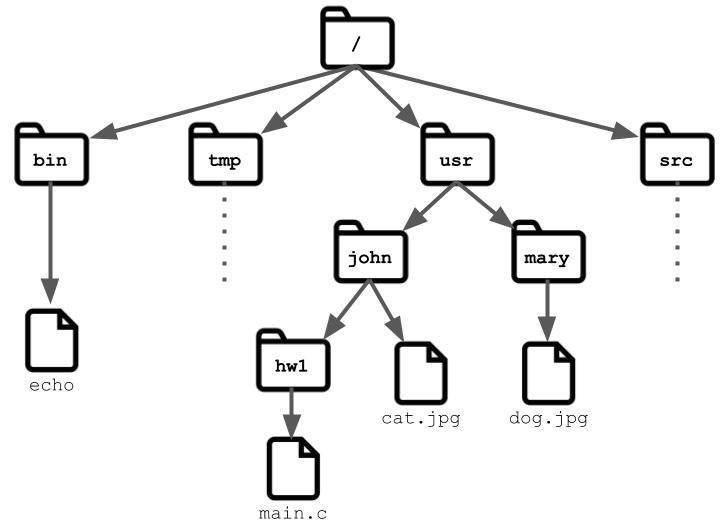
\includegraphics[width=.6\textwidth]{images/file_system.png}
\label{fig:exampleFig2}
\end{figure}

Expressões matemáticas com operadores binários podem ser representados utilizando árvores de expressões. Na figura \ref{fig::tree_expression}, mostra a árvore de expressão da (a+b)*c+7.

\begin{figure}[htbp]
\centering
\label{fig::tree_expression}
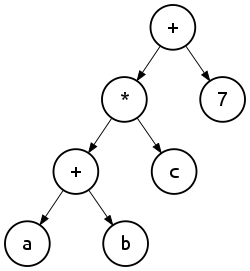
\includegraphics[scale=0.5]{images/250px-Exp-tree-ex-11.svg.png}
\label{fig:exampleFig2}
\caption{Árvore de expressão da expressão (a+b)*c+7}
\end{figure}

A representação de uma expressão no formato de árvore tem algumas vantagens importantes:

\begin{itemize}
    \item A árvore de expressão não precisa guardar delimitadores e símbolos de pontuação.
    \item A representação hierárquica deixa claro a ordem de avaliação dos operadores.
    \item Você pode guardar informações extra sobre os operandos e operadores na árvore de expressão.
\end{itemize}



\section{Árvore de Expressão}

Uma expressão aritmética é uma sequência de texto que possui estrutura de recursiva de formação. Uma expressão aritmética pode ser construída a partir de números, variáveis, operadores binários como +,-,* e / e alguns símbolos de pontução como '(' e ')'. 

Uma expressão aritmética (EXP) pode ser definida da seguinte maneira:

\begin{itemize}
\item Seja $\alpha$ uma sequência de texto representando um número então $\alpha \in EXP$.
\item Seja $\alpha$ uma sequência de texto representando uma variável então $\alpha \in EXP$.
\item Seja $\alpha, \beta \in EXP$  então $\alpha + \beta \in EXP, \alpha - \beta \in EXP, \alpha * \beta \in EXP$ e $\alpha / \beta \in EXP$.
\end{itemize} 


Para construir uma estrutura de dados para representar uma expressão dada, precisamos construir uma árvore onde cada nó da árvore pode ser qualquer uma das diferentes formas que essa expressão pode assumir. Por exemplo, em um árvore de expressão aritmética, um nó pode representar uma constante, uma variável ou uma operação binária como a soma, subtração, multiplicação ou divisão. Observe que cada esses tipos de nós tem uma quantidade de filhos diferentes.

Uma maneira de definir essa estrutura de dados é construir uma única classe para os nós com todas as informações para os diferentes tipos de nós como um rótulo para indicar cada tipo de nó da seguinte maneira:

\begin{minted}
[
frame=lines,
bgcolor=LightGray,
fontsize=\footnotesize,
linenos
]
{C++}
class exp {
    public:
    typedef enum { NUM, VAR, BINOP} exp_type;
    exp_type type;
    int value;
    string name;
    char op;
    exp * left;
    exp * right;
    exp(int value);
    exp(string name);
    exp(char op, exp * left, exp * right);
};
\end{minted}

A função para imprimir uma árvore de expressão seria da seguinte maneira:


\begin{minted}
[
frame=lines,
bgcolor=LightGray,
fontsize=\footnotesize,
linenos
]
{C++}
void print(exp * e){
    switch(e->type){
        case exp::NUM:
            cout << e->value;
            break;
        case exp::VAR:
            cout << e->name;
            break;
        case exp::BINOP:
            print(e->left);
            cout << e->op;
            print(e->right);
            break;
    }

}
\end{minted}

Essa implementação possui algumas desvantagens:

\begin{itemize}
\item Como temos apenas uma classe para representar os diferentes tipos de nós, qualquer alteração ou extensão precisar alterar essa classe.
\item A quantidade de filhos não interfere na quantidade de memória utilizada para cada nó.
\item Ao usar um nó, precisamos sempre checar seu rótulo para realizar as operações de maneira adequada.
\end{itemize}

Uma outra maneira de implementar uma árvore de expressão é utilizando uma hierarquia de herança dos diferentes tipos de nós de uma árvore de expressão. Vamos definir uma classe base e em seguida adicionar as subclasses, uma para cada tipo de nó.

Classe Base:

\begin{minted}
[
frame=lines,
bgcolor=LightGray,
fontsize=\footnotesize,
linenos
]
{C++}
class exp {
    public:
    virtual void print() = 0; // Pure virtual
};
\end{minted}

Hierarquia de Herança:

\begin{minted}
[
frame=lines,
bgcolor=LightGray,
fontsize=\footnotesize,
linenos
]
{C++}
class exp_num : public exp {
    int value;
    public:
    exp_num(int value);
    virtual void print() {
        cout << value;
    }
};

class exp_var : public exp {
    
    string name;
    public:
    exp_var(string name);
    virtual void print() {
        cout << name;
    }
};


struct exp_op : public exp {
    char op;
    exp* left;
    exp* right;
    public:
    exp_op(char op, exp * left, exp * right);
    virtual void print() {
        left->print();
        cout << op;
        right->print();
    }
};

\end{minted}

Uma árvore de expressão pode ser construída da seguinte maneira:
\begin{minted}
[
frame=lines,
bgcolor=LightGray,
fontsize=\footnotesize,
linenos
]
{C++}
    exp * e =   new exp_op('+', 
                new exp_num(2),
                new exp_num(3)
                );
    e->print();

\end{minted}

\section{Construindo uma árvore de expressão}

Considere uma expressão na notação polonesa reversa (notação pós-fixa). A construção da árvore de expressão pode ser realizada com as seguintes regras:

\begin{enumerate}
    \item Se o símbolo é operando então crie um ponteiro para nó da árvore para o operando e empilhe um ponteiro para um nó representado pelo operando.
    \item Se o símbolo é um operador binário, desempilhe dois ponteiros para nós e empilhe na pilha um ponteiro para um nó representando o operador binário com dois filhos.
\end{enumerate}

Considere o processo de criação da árvore de expressão para a seguinte expressão: a b + c d e + * * 


\begin{enumerate}

\item Dois ponteiros para nós são criados para os dois primeiros operandos e empilhados na pilha.

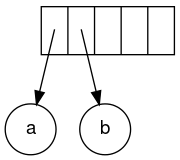
\includegraphics[scale=0.5]{images/passo1.png}

\item Um operador é encontrado, dois ponteiros são retirados da pilha e um novo nó é empilhado.

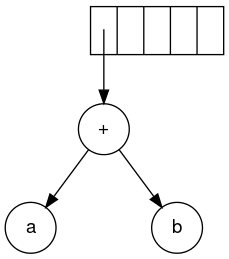
\includegraphics[scale=0.5]{images/passo2.png}

\item Três ponteiros para nós são criados para os próximos três operandos e eles são empilhados na pilha.

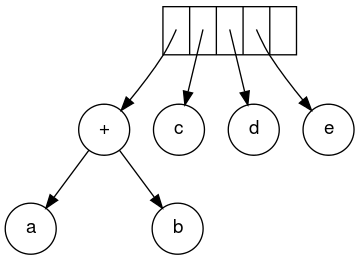
\includegraphics[scale=0.5]{images/passo3.png}

\item Um operador é encontrado, dois ponteiros são retirados da pilha e um novo ponteiro nó é empilhado.

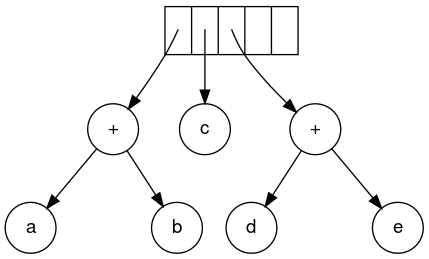
\includegraphics[scale=0.5]{images/passo4.png}

\item Um operador é encontrado, dois ponteiros são retirados da pilha e um novo ponteiro nó é empilhado.

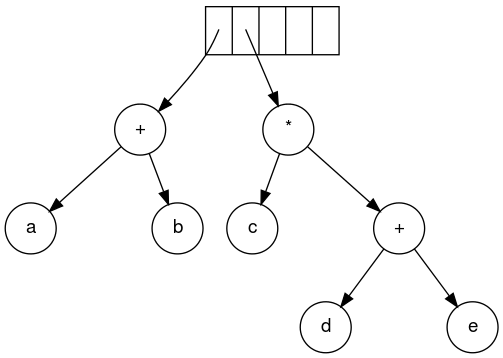
\includegraphics[scale=0.5]{images/passo5.png}

\item Um operador é encontrado, dois ponteiros são retirados da pilha e um novo ponteiro para nó é empilhado.

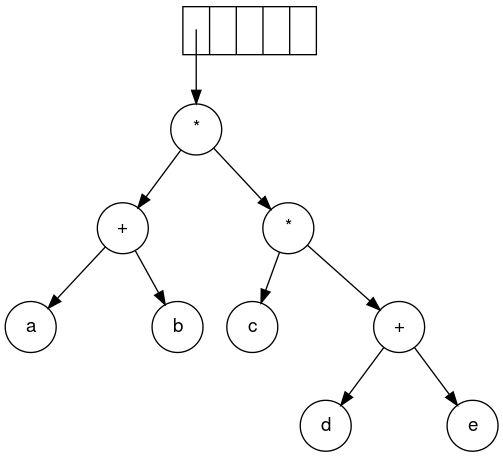
\includegraphics[scale=0.5]{images/passo6.png}


\end{enumerate}



\begin{minted}
[
frame=lines,
bgcolor=LightGray,
fontsize=\footnotesize,
linenos
]
{C++}
exp * read_postfix(vector <string> tokens){
    stack <exp *> st;

    for(string t : tokens){
        if( is_numeric(t) ){
            st.push( new exp_num(stoi(t)) );
        }
        else if( is_variable(t) ){
            st.push( new exp_var(t) );
        }else if( is_op(t) ){
            exp * r = st.top(); st.pop();
            exp * l = st.top(); st.pop();
            st.push( new exp_op(t.front(), l, r) );
        } 
    }
    return st.top();
}
\end{minted}



\section{Expressão Lógica}

Uma expressão lógica é uma sequência de texto que utiliza constantes (true, false), variáveis proposicionais e operadores lógicos como ($\neg, \wedge, \vee, \to, \leftrightarrow$).

O conjunto da expressões lógicas (EXPLOG) bem-formadas pode ser definido da seguinte maneira:

\begin{itemize}
    \item Se $\alpha$ é uma constante, então $ \alpha\in  EXPLOG$.
    \item Se $\alpha$ é uma variável proposicional, então $ \alpha\in  EXPLOG$.
    \item Se $\alpha \in EXPLOG$ então 
    $$\neg \alpha \in EXPLOG$$.
    \item Se $\alpha,\beta \in EXPLOG$ então 
    $$\alpha \vee \beta, \alpha \wedge \beta, \alpha \to \beta, \alpha \leftrightarrow \beta$$.
\end{itemize}

Novamente, vamos recorrer uma hierarquia de herança para representar uma expressão lógica da seguinte maneira:


\begin{minted}
[
frame=lines,
bgcolor=LightGray,
fontsize=\footnotesize,
linenos
]
{C++}
class logical {
  public:
    virtual void print() = 0;
    
};

class log_const : public logical {
  public:
    log_const(bool value) : value(value) {}
    void print() { 
        cout << value ? "true" : "false";
    }
  private:
    bool value;
};

class log_prop : public logical {
  public:
    log_prop(string name) : name(name) {}
    
    void print() {
        cout << name;
    }
  private:
    string name;
};

class log_neg : public logical {
  public:
    log_neg(logical * inner) : inner(inner) {}
    void print() {
        cout << "~";
        inner->print();
    }
    
  private:
    logical* inner;
};

class log_op : public logical {
  public:
    log_op(string op, logical * l, logical * r) : op(op), left(l), right(r) {}
    void print() {
        cout << "("; left->print(); cout << op; right->print(); cout << ")";
    }
  private:
    string op;
    logical * left;
    logical * right;
};

\end{minted}

O processo de construção de uma árvore de expressão lógica a partir de uma expressão na notação pós-fixa segue o mesma ideia:


\begin{minted}
[
frame=lines,
bgcolor=LightGray,
fontsize=\footnotesize,
linenos
]
{C++}
logical * read_postfix(vector <string> tokens){
    stack <logical *> st;

    for(string t : tokens){
        
        if( is_bool(t) ){
            
            st.push( new log_const( t == "true" ) );
        }
        else if( is_variable(t) ){
            
            st.push( new log_prop(t) );
        }else if( t == "~"){
            logical * inner = st.top(); st.pop();
            st.push( new log_neg(inner) );
        }
        else if( is_op(t) ){
            logical * r = st.top(); st.pop();
            logical * l = st.top(); st.pop();

           
            st.push( new log_op(t , l, r) );
        } 
    }
    return st.top();
}
\end{minted}

Imagine que você queira encontrar uma expressão lógica equivalente sem a utilização do operador $\to$. Você pode utilizar a seguinte regra de equivalência:

$$
\alpha \to \beta \equiv \neg \alpha \vee \beta
$$

O processo de remoção do implicação pode ser definido de maneira recursiva. Seja REMOVE\_IMPLIES($\alpha$) uma função que devolve uma expressão lógica equivalente a $\alpha$ sem o operador $\to$.

\begin{itemize}
    \item Se $\alpha$ é uma constante, então $REMOVE\_IMPLIES(\alpha) = \alpha$.
    \item Se $\alpha$ é uma variável proposicional, então $REMOVE\_IMPLIES(\alpha) = \alpha$.
    \item Se $\neg \alpha \in EXPLOG$ então 
    $$REMOVE\_IMPLIES(\neg \alpha) = \neg REMOVE\_IMPLIES(\alpha)$$
    \item Se $\alpha \vee \beta \in EXPLOG$ então 
    $$REMOVE\_IMPLIES(\alpha \vee \beta) = REMOVE\_IMPLIES(\alpha) \vee REMOVE\_IMPLIES(\beta)$$.
    \item Se $\alpha \wedge \beta \in EXPLOG$ então 
    $$REMOVE\_IMPLIES(\alpha \wedge \beta) = REMOVE\_IMPLIES(\alpha) \wedge REMOVE\_IMPLIES(\beta)$$.
    \item Se $\alpha \leftrightarrow \beta \in EXPLOG$ então 
    $$REMOVE\_IMPLIES(\alpha \leftrightarrow \beta) = REMOVE\_IMPLIES(\alpha) \leftrightarrow REMOVE\_IMPLIES(\beta)$$.
    \item Se $\alpha \to \beta \in EXPLOG$ então 
    $$REMOVE\_IMPLIES(\alpha \to \beta) = \neg REMOVE\_IMPLIES(\alpha) \vee REMOVE\_IMPLIES(\beta)$$.
\end{itemize}

Essa função pode ser implementada sem utilizar a hierarquia de herança da seguinte maneira:

\begin{minted}
[
frame=lines,
bgcolor=LightGray,
fontsize=\footnotesize,
linenos
]
{C++}
logical * remove_implies(logical * exp){

  log_neg * exp_neg = dynamic_cast<log_neg*>(exp);

  if( exp_neg != nullptr){
    
    return new log_neg( remove_implies( exp_neg->inner) );
  }
  else{
    log_op * exp_op = dynamic_cast<log_op*>(exp);

    if( exp_op == nullptr)
    {
      return exp;
    }
    else
    {
      logical * l = remove_implies( exp_op->left );
      logical * r = remove_implies( exp_op->right);
        
      if( exp_op->op == "->")
      {  
        return new log_op("\\/", new log_neg(l), r);
      }
      else
        return new log_op(exp_op->op, l, r);
    }
  }

}

\end{minted}


\section{Árvore Binária}

Uma árvore binária é uma estrutura de dados genéricas para representar uma relação hierárquica em que cada nó tem no máximo 2 filhos. Na nossa modelagem, uma árvore binária será representada por um classe TreeNode com um valor que chamaremos key e dois ponteiros para TreeNode chamado left, right. 


\begin{minted}
[
frame=lines,
bgcolor=LightGray,
fontsize=\footnotesize,
linenos
]
{C++}
template <typename T> 
class NodeTree{
    public:
    T key;
    NodeTree<T> * left;
    NodeTree<T> * right;
    NodeTree(T key) : key(key), left(nullptr), right(nullptr) {};
    NodeTree(T key, NodeTree * l, NodeTree * r) : key(key), left(l), right(r) {};    
};
\end{minted}


A primeira função que criaremos será a função \texttt{createTree}. Essa função vai receber um vector keys com as chaves que serão armazenadas na árvore e um outro vector parent guardando o índice do nó pai para nó da árvore. Inicialmente, criaremos um vetor de nós da árvore. Para cada valor no vector keys, criaremos uma nó de uma árvore. Note que os dois ponteiros dos filhos da esquerda (left) e direita (right) vão ser inicializados com nullptr. A medida que fomos processando o vector parent, colocaremos o primeiro nó filho na esquerda e o segundo ó filho na direita.


\begin{minted}
[
frame=lines,
bgcolor=LightGray,
fontsize=\footnotesize,
linenos
]
{C++}
template <typename T> 
NodeTree<T> * createTree( vector<T> keys, vector<int> parent){

    NodeTree<T>* tree[keys.size()];
    NodeTree<T>* root;
    for(int i = 0; i < keys.size(); i++){
        tree[i] = new NodeTree<T>(keys[i]);
    }
    for(int i = 0; i < keys.size(); i++){
        if( parent[i] == -1)
            root = tree[i];
        else
        {
            NodeTree<T>* ptr = tree[ parent[i] ];
            if( ptr->left ){
                ptr->right = tree[i];
            }else{
                ptr->left = tree[i];
            }
        }
    }
    return root;
} 

\end{minted}

Em seguida, construíremos uma função \tetxtt{dotfile} para escrever um arquivo no formato dot para facilitar a visualização da nossa árvore binária:

\begin{minted}
[
frame=lines,
bgcolor=LightGray,
fontsize=\footnotesize,
linenos
]
{C++}

template <typename T>
void dotfileaux(ofstream & ofs, NodeTree<T> * ptr);


template <typename T>
void dotfile(NodeTree<T> * ptr)
{
    ofstream ofs ("bt.dot", ofstream::out);

    ofs << "digraph G {" << endl;

    dotfileaux(ofs, ptr);

    ofs << "}" << endl;

    ofs.close();

}

template <typename T>
void dotfileaux(ofstream & ofs, NodeTree<T> * ptr){
    static int nullcount = 0;
    if(ptr != nullptr){
        if(ptr->left){
            ofs << ptr->key << "->" << ptr->left->key  << ";" << endl;
            dotfileaux(ofs, ptr->left);
        }else{
            ofs << "null" << nullcount << " [shape=point];" << endl;
            ofs << ptr->key << "->" << "null" << nullcount << ";" << endl; 
            nullcount++;
        }
        if(ptr->right != nullptr){
            ofs << ptr->key << "->" << ptr->right->key  << ";" << endl;
            dotfileaux(ofs, ptr->right);
        }else{
            ofs << "null" << nullcount << " [shape=point];" << endl;
            ofs << ptr->key << "->" << "null" << nullcount << ";" << endl; 
            nullcount++;
        }
    }
} 

\end{minted}

Considerando a seguinte programa principal:


\begin{minted}
[
frame=lines,
bgcolor=LightGray,
fontsize=\footnotesize,
linenos
]
{C++}

int main(){
    vector<int> keys( {0,1,2,3,4,5,6,7});
    vector<int> parent({-1,0,0,1,2,2,4,4});
    auto root = createTree(keys, parent);
    dotfile(root);
}
\end{minted}

O programa principal acima escreve o seguinte arquivo dot:


\begin{minted}
[
frame=lines,
bgcolor=LightGray,
fontsize=\footnotesize,
linenos
]
{C++}

digraph G {
0->1;
1->3;
null0 [shape=point];
3->null0;
null1 [shape=point];
3->null1;
null2 [shape=point];
1->null2;
0->2;
2->4;
4->6;
null3 [shape=point];
6->null3;
null4 [shape=point];
6->null4;
4->7;
null5 [shape=point];
7->null5;
null6 [shape=point];
7->null6;
2->5;
null7 [shape=point];
5->null7;
null8 [shape=point];
5->null8;
}
\end{minted}

Você pode utilizar algum visualizador online de arquivos no formato dot \footnote{ \url{ https://dreampuf.github.io/GraphvizOnline/}} obtendo a seguinte imagem:

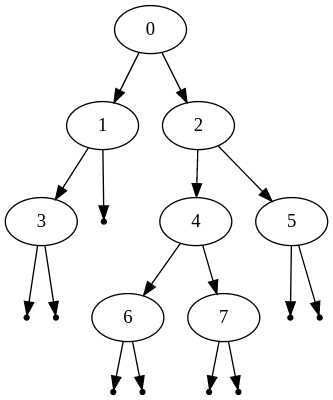
\includegraphics[scale=0.5]{images/graphviz.png}

Podemos implementar algumas funções para responder algumas perguntas sobre a nossa árvore. Por exemplo, podemos calcular o número de nós da nossa árvore.

\begin{minted}
[
frame=lines,
bgcolor=LightGray,
fontsize=\footnotesize,
linenos
]
{C++}

template <typename T> 
int btsize(NodeTree<T> * ptr){
    if(ptr == nullptr)
        return 0;
    else
        return 1 + btsize(ptr->left) + btsize(ptr->right);
}
\end{minted}


Um nó é dito ser um nó folha quando ele não possui nenhum filho (as subárvores da esquerda e direita apontam para nullptr).
A altura de um nó $v$ é o número de nós do maior caminho do nó $v$ até um nó folha descendente de $v$. A altura de uma árvore é a altura do nó raiz da árvore. 
\begin{minted}
[
frame=lines,
bgcolor=LightGray,
fontsize=\footnotesize,
linenos
]
{C++}

template <typename T> 
int btheight(NodeTree<T> * ptr){
    if(ptr == nullptr)
        return 0;
    else
        return 1 + max( btheight(ptr->left), btheight(ptr->right) );
}
\end{minted}

A profundidade de um nó $v$ é o número de nó no caminho do nó $v$ até o nó raiz. A seguinte Figura mostra uma árvore a altura e a profundidade de cada nó da árvore:

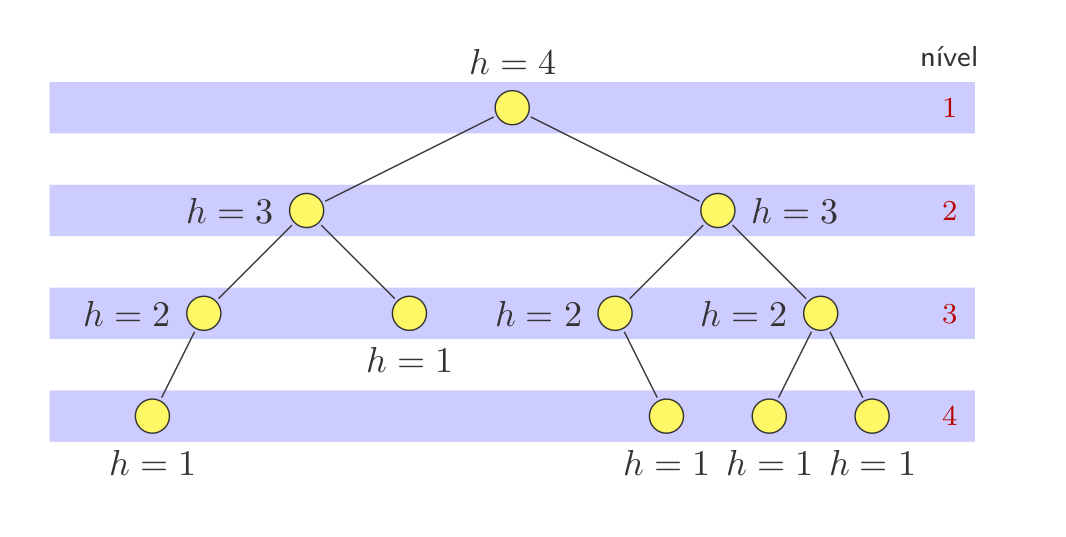
\includegraphics[scale=0.3]{images/altura.png}

\subsection{Árvore Binária Estrita}

Uma árvore binária é dita estrita quando todos os nós possuem 0 ou 2 filhos.

Seja i o número de nós internos de uma árvore binária T, n o número total de nós, l o número de folhas e $\lambda$ o número de níveis. As seguintes propriedades valem para uma árvore binária estrita:

\begin{itemize}
    \item $l = i+1$
    \item  $n = 2*i + 1$
    \item $i = (n-1)/2$
    \item $n = 2l - 1$
    \item $i = l-1$
    \item $l \leq 2\lambda - 1$
\end{itemize}





\subsection{Árvore Binária Perfeita}

Uma árvore binária é dita cheia ou perfeita se todos os nós internos tem duas folhas e todas as folhas estão no último nível.

As seguintes propriedades valem para uma árvore binária cheia:

\begin{enumerate}
    \item Se uma árvore binária cheia tem altura h então ela possui $2^{h-1}$ folhas.
    \item Se uma árvore binária cheia tem altura h então possui $2^{h} - 1$ nós.
\end{enumerate}


\fcolorbox{black}{lightblue}{
\begin{minipage}{\textwidth}
\begin{theorem}
Seja $T$ uma árvore binária cheia com altura $h$ então $T$ possui $2^{h} - 1$ nós folhas.
\end{theorem}

\begin{proof}
Considere que folhas(T) é uma função que devolve a quantidade de folhas de uma árvore de uma árvore binária T qualquer. Vamos provar por indução na altura da árvore binária cheia $T$. Se T tem altura 1, então T possui $2^{1-0}$ folhas. Por hipótese, sabemos que uma árvore binária cheia T de altura k possui $2^{k-1}$ folhas. Seja $T'$ uma árvore com altura k+1. Pela construção de uma árvore binária cheia, sabemos que as duas subárvores da esquerda e direita, respectivamente, $T_1$ e $T_2$ são cheias e possuem altura k. Por hipótese, temos que $folhas(T_1)= 2^{k-1}$ e $folhas(T_2)= 2^{k_1-1}$. Assim, 

$$folhas(T) = folhas(T_1) + folhas(T_2)$$

Dessa maneira, $folhas(T) = 2^{k} = 2^{k+1-1}$
\end{proof}


\begin{theorem}
Seja $T$ uma árvore binária cheia com altura $h$ então $T$ possui $2^{h} - 1$ nós.
\end{theorem}

\begin{proof}
Sabemos que:
\begin{itemize}
    \item Uma árvore de cheia possui $2^{0}$ nó no nível 1.
    \item Uma árvore de cheia possui $2^{2-1}$ nós no nível 2.
    \item $\ldots$
    \item Uma árvore de cheia possui $2^{h-1}$ nós no nível h.
\end{itemize}
Logo, o total de nós é $1 + 2 + \ldots 2^{h-1} = 2^h -1$
\end{proof}


\end{minipage}
}


Nós podemos usar a propriedade (2) para verificar se uma árvore binária é cheia utilizando as funções btheight e btsize.

\begin{minted}
[
frame=lines,
bgcolor=LightGray,
fontsize=\footnotesize,
linenos
]
{C++}

template <typename T>
bool is_perfect_binary(NodeTree<T> * ptr)
{
    int h = btheight(ptr);
    int n = btsize(ptr);
    return n == (1 << h) - 1;
}
\end{minted}

A seguinte árvore binária é cheia:


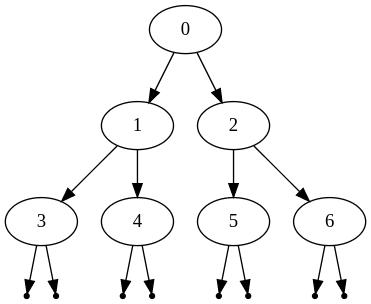
\includegraphics[scale=0.3]{images/cheia.png}

Analisando a árvore binária acima, podemos fazer uma bijeção entre a posição de um nó na árvore e a sua posição em um vetor unidimensional da seguinte maneira:

\begin{itemize}
    \item A chave da raiz será colocado na posição 0.
    \item Se a chave de um nó está na posição $i$, então a chave do filho da esquerda será colocado na posição $2i+1$ e o filho da direita será colocado na posição $2i+2$.
\end{itemize}

\subsection{Árvore Binária Completa}

Em alguns casos, a quantidade de nós não é suficiente para formar uma árvore binária cheia. Neste caso, podemos construir uma árvore binária completa. Uma árvore binária completa é uma árvore binária em que todos os níveis estão completo exceto o último nível que é preenchido da esquerda para a direita. A seguir, temos uma imagem de uma árvore completa:


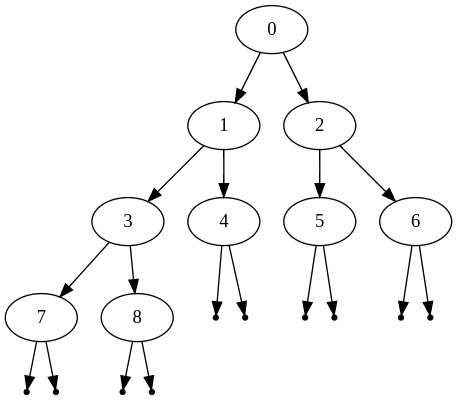
\includegraphics[scale=0.3]{images/completa.png}

Para checar se uma árvore é completa, exploraremos a relação entre a posição do nó e o seu índice em um vetor unidimensional.

\begin{minted}
[
frame=lines,
bgcolor=LightGray,
fontsize=\footnotesize,
linenos
]
{C++}

template <typename T>
bool is_complete_binary(NodeTree<T> * ptr, int index, int numnodes)
{
    if(ptr == nullptr)
        return true;
    if( index > numnodes-1)
        return false;
    else
        return  is_complete_binary(ptr->left, 2*index+1, numnodes) &&
                is_complete_binary(ptr->right, 2*index+2, numnodes);
}
\end{minted}





\chapter{Árvore binária de busca }

Uma árvore binária de busca é uma estrutura de dados de árvore binária enraizada tal que para cada nó interno da árvore armazena uma chave maior que todos os nós da esquerda e menor que os todos os nós da direita. Como um mesmo conjunto de valores de chaves podemos construir várias árvore de busca binária. No exemplo abaixo, temos duas árvore de busca binária formada pelos valores de chaves \{5,10,12,15,20,25\}:

\includegraphics[width=.6\textwidth]{images/9-5.png}

Uma árvore binária de busca com $n$ nós pode ter uma altura h variando entre  $ \lceil log~ (n+1)  \rceil \leq h \leq n$.

Nessa estrutura de dados, a complexidade de tempo para realizar as operações de busca, inserção e remoção são proporcionais a altura da árvore. Por isso, estamos interessados em trabalhar com uma árvore de busca com a altura próxima de $log~ n$. No exemplo acima, as operações de busca, inserção e remoção são mais demorado na árvore binária de busca da direita do que na esquerda. Contudo, as alturas das duas árvores estão próximas de $log ~n$. O nosso primeiro problema será construir uma árvore binária de busca com uma altura próxima $log~ n$ a partir de um conjunto de chaves.

Inicialmente, vamos realizar uma ordenação do nosso conjunto de chaves. 

\begin{minted}
[
frame=lines,
bgcolor=LightGray,
fontsize=\footnotesize,
linenos
]
{C++}
template <typename T> 
NodeTree<T>* createCompleteTree(vector <T> keys){
    sort(keys.begin(), keys.end() );
    return createCompleteTreeAux(keys);
}
\end{minted}


Durante o processo de criação da nossa árvore binária de busca, escolheremos o elemento do meio como raiz da nossa árvore de busca. Em seguida, as chaves $keys[0..mid-1]$ serão usadas para criar a subárvore da esquerda e as chaves $keys[mid+1, keys.size()-1]$ serão usadas para criar a subárvore da direita.

\begin{minted}
[
frame=lines,
bgcolor=LightGray,
fontsize=\footnotesize,
linenos
]
{C++}

template <typename T> 
NodeTree<T>* createCompleteTreeAux(vector <T> keys){
    int n = keys.size();
    if(n == 0){
        return nullptr;
    }else if(n == 1){
        return  new NodeTree<T>( keys[0] );
    }else{
        int mid = n/2;

        NodeTree<T>* root = new NodeTree<T>( keys[mid] );

        vector <T> leftkeys;
        vector <T> rightkeys;

        leftkeys.assign( keys.begin(), keys.begin() + mid);
        rightkeys.assign( keys.begin() + mid + 1, keys.end() );

        root->left  = createCompleteTreeAux(leftkeys);
        root->right = createCompleteTreeAux(rightkeys);

        return root;
    }
}
\end{minted}

Dessa maneira, conseguimos construir uma árvore de busca com a complexidade de tempo $O(n~ log~ n)$.

A operação de busca em um árvore binária de busca pode tirar proveito da estrutura da árvore binária de busca para realizar uma busca baseada no mesmo princípio da busca binária.

\begin{minted}
[
frame=lines,
bgcolor=LightGray,
fontsize=\footnotesize,
linenos
]
{C++}
template <typename T> 
NodeTree<T> * search(NodeTree<T> * root, T key){
    if(root == nullptr)
        return nullptr;
    else{
        if( root->key == key )
            return root;
        else if( key < root->key)
            return search(root->left, key);
        else 
            return search(root->right, key);
    }
}
\end{minted}

Note que se a nossa chave de busca (key) for menor que a chave da raiz da árvore (root->key) então o nó contendo a chave key (se ela existir) estará na subárvore da esquerda. Se a chave for maior que a chave da raiz da árvore, então o nó com essa chave deve estar na subárvore da direita.

A operação de inserção na árvore de busca segue uma idéia semelhante do processo de busca contudo o algoritmo de inserção apresentado não é capaz de manter a altura da árvore no seu valor mínimo.


\begin{minted}
[
frame=lines,
bgcolor=LightGray,
fontsize=\footnotesize,
linenos
]
{C++}
template <typename T> 
template <typename T> 
NodeTree<T>* insert(NodeTree<T> * root, T key){
    if(root == nullptr)
        return new NodeTree<T>(key);
    else{
        if( key < root->key ){
            root->left = insert(root->left, key);
        }else{
            root->right = insert(root->right, key);
        }
        return root;
    }
}
\end{minted}

Considere a seguinte árvore construída com o seguinte conjunto de chaves \{4,6,7,2,3,10,12,9,-5, 8\} utilizando o algoritmo acima:

\begin{figure}
    \centering
    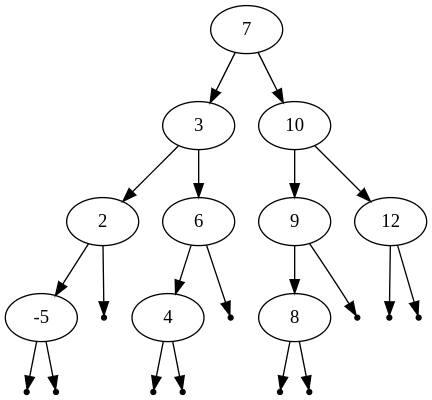
\includegraphics[scale=0.5]{images/bst.png}

    \caption{Árvore binária de busca formada pelas chaves \{4,6,7,2,3,10,12,9,-5, 8\} }
    \label{fig::bst1}
\end{figure}

Se você inserir as chaves {-4,-3}, aumentaremos a altura da árvore em duas unidades.

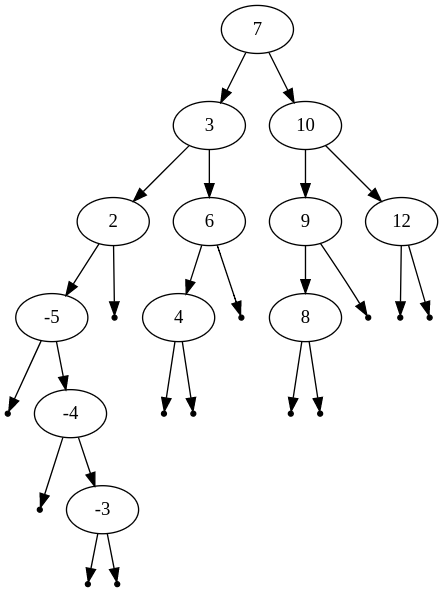
\includegraphics[scale=0.5]{images/bst2.png}

Esse problema será resolvido desenvolvendo uma função de inserção na árvore de busca capaz de manter a altura da árvore em  $O(log ~n)$

A operação de remoção em uma árvore binária de busca pode ser realizada da seguinte maneira:

\begin{enumerate}
    \item Primeiramente, encontraremos o nó raiz da subárvore (node) que será alterada.
    \begin{enumerate}
    \item Se node->right for nullptr, então salvamos o node->left em q, deletamos node e devolvemos q. Note que se  node->left for nullptr então significa que node não tem filhos e que node pode ser simplesmente removida e árvore resultante é vazia. Se node->left for diferente de nullptr, então node->left será a raiz da árvore resultante da remoção de node.
    \item Se node->right for diferente de nullptr, precisamos encontrar o sucessor de node e o seu pai para encontrar a árvore resultante da remoção de node. O nó sucessor será o nó com o menor valor da subárvore da direita. O nó com o menor valor será o nó que está mais à esquerda da subárvore da direita. Na Figura \ref{fig::bst1}, o sucessor do nó com chave 7 é o nó com chave 8 que é o nó mais à esquerda da subárvore da direita do nó com chave 7.
    
    
    Temos que considerar dois novos casos:
        \begin{enumerate}
        \item Se o nó pai do sucessor for igual ao nó a ser removido, então precisamos colocar o nó sucessor como raiz da árvore resultante da remoção de node e a esquerda do nó sucessor será ajustada para a esquerda do nó a ser removido.
        \item Se o nó pai do sucessor for diferente ao nó a ser removido, ajustaremos a esquerda do nó pai para a direita do nó sucessor. Em seguida, colocaremos o nó sucessor como raiz da subárvore resultante da remoção de nó node.
        
        \end{enumerate}
        
    \end{enumerate}
\end{enumerate}

O código que reflete a ideia acima é o seguinte:

\begin{minted}
[
frame=lines,
bgcolor=LightGray,
fontsize=\footnotesize,
linenos
]
{C++}
template <typename T> 
NodeTree<T> * removeRoot(NodeTree<T> * node){

    if( node->right == nullptr){
        NodeTree<T> * q = node->left;
        delete node;
        return q;
    }else{
        
        NodeTree<T> * pai  = node; 
        NodeTree<T> * succ = node->right;

        while( succ->left != nullptr){
            pai = succ;
            succ = succ->left;
        }

        if( pai == node ){
            succ->left = node->left;
            delete node;
            return succ;
        }else{
            pai->left = succ->right;
            succ->right = node->right;
            succ->left  = node->left;
            delete node;
            return succ;
        }
        
    }
}

template <typename T> 
NodeTree<T> * remove(NodeTree<T> * root, T key){
    
    if(root == nullptr)
        return nullptr;
    else if( root->key == key ){
        return removeRoot(root);
    }else if( key < root->key ){
        root->left = remove(root->left, key);
    }else {
        root->right = remove(root->right, key);
    }
    return root;
}
\end{minted}

Podemos adicionar o campo size a nossa NodeTree e garantir que as operações de inserção e remoção da árvore mantenham esse campo bem calculado.

\begin{minted}
[
frame=lines,
bgcolor=LightGray,
fontsize=\footnotesize,
linenos
]
{C++}
template <typename T> 
NodeTree<T>* insert(NodeTree<T> * root, T key){
    if(root == nullptr)
        return new NodeTree<T>(key);
    else{
        if( key < root->key ){
            root->left = insert(root->left, key);
            root->size++;
        }else{
            root->right = insert(root->right, key);
            root->size++;
        }
        return root;
    }
}
\end{minted}

O mesmo pode ser realizado na função remove:

\begin{minted}
[
frame=lines,
bgcolor=LightGray,
fontsize=\footnotesize,
linenos
]
{C++}

template <typename T> 
NodeTree<T> * remove(NodeTree<T> * root, T key){
    
    if(root == nullptr)
        return nullptr;
    else if( root->key == key ){
        return removeRoot(root);
    }else if( key < root->key ){
        root->left = remove(root->left, key);
        root->size--;
    }else {
        root->right = remove(root->right, key);
        root->size--;
    }
    return root;
}
\end{minted}

As alterações que devem ser realizadas na função removeRoot serão deixadas para o leitor.



\chapter{Heap}

A estrutura de dados \textbf{heap} pode ser entendida como uma vetor de chaves que podem ser visto como uma árvore binária completa com uma propriedade adicional. Cada nó dessa árvore corresponde a um elemento do vetor $keys$ que armazena o valor.  Dado um vetor, podemos construir uma árvore binária completa da seguinte maneira:

\begin{minted}
[
frame=lines,
bgcolor=LightGray,
fontsize=\footnotesize,
linenos
]
{C++}
#define left(i) 2*i + 1 
#define right(i) 2*i + 2
#define parent(i) ((i-1)/2)

template <typename T> 
NodeTree<T> * createCompleteTree(vector<T> keys, int index = 0){
    if( index > keys.size()-1 )
        return nullptr;
    else{
        auto left  = createCompleteTree(keys, left(index)); 
        auto right = createCompleteTree(keys, right(index));
        return new NodeTree(keys[index], left, right);
    }
} 
\end{minted}

Utilizando o algoritmo acima, o conjunto de chaves $keys = \{30,10,45,78,12,63,36\}$

\includegraphics[width=.6\textwidth]{images/heap.png}

Queremos que o valor associado a cada nó da árvore binária seja menor que o valor do associado ao seu nó pai.

Essa propriedade pode ser verificada checando:

$$
keys[ parent(i) ] \geq keys[i] \quad \forall i \in [1,\ldots, keys.size()-1]
$$

\section{Função heapify}

A função heapify é uma subrotina responsável para construção de um heap máximo. Ela recebe como entrada um vetor arr, o tamanho atual do heap (heapsize) e um inteiro $i$. Assumimos que as árvores binárias com raiz left(i) e right(i) são heap máximos, mas que $arr[i]$ pode estar violando a propriedade de heap máximo. Se a propriedade de heap máximo for violada, colocamos o maior valor para a raiz da árvore com raiz no índice $i$ e descemos o valor $arr[i]$ para um dos seus filhos. Com a descida do valor $arr[i]$ para um dos filhos, a subárvore com a raiz nesse filho pode ter a sua propriedade violada. Como a árvore binária induzida pelo vetor de valores possui uma altura $O(log n)$. A função heapify executa no tempo $O(log~ n)$


\begin{minted}
[
frame=lines,
bgcolor=LightGray,
fontsize=\footnotesize,
linenos
]
{C++}
void heapify(vector<int> & arr, int heapsize, int i){
    int l = left(i);
    int r = right(i);
    int maior;
    cout << "heapify" << i << endl;
    if( l < heapsize && arr[l] > arr[i]){
        maior = l;
    }else{
        maior = i;
    }
    
    if(r < heapsize && arr[r] > arr[maior]){
        maior = r;
    }
    if(maior != i ){
        swap(arr[maior], arr[i]);
        heapify(arr, heapsize, maior);
    }
}
\end{minted}

\section{build heap}

A função build heap é uma função responsável por converter um vector arr de tamanho arr.size() em um heap máximo. Como a função heapify assume que as subárvores binárias construídas pelos índices left(i) e right(i) precisam ser heap máximos. O processo de construção será realizado de baixo para cima. Na árvore binária completa inicial, temos que $\lceil n/2 \rceil$ são folhas, ou seja, são subárvores que representam heap máximos. A quantidade de nós internos em uma árvore binária completa é $\lfloor n/2 \rfloor$.

\begin{minted}
[
frame=lines,
bgcolor=LightGray,
fontsize=\footnotesize,
linenos
]
{C++}
void build_heap(vector <int> & arr, int heapsize)
{
    for(int i = floor(heapsize/2); i >= 0; i--){
        heapify(arr, heapsize, i);
    }
}

\end{minted}

\fcolorbox{black}{lightblue}{
\begin{minipage}{\textwidth}
Prove que em uma árvore binária completa com $n$ nós possui $\lceil n/2 \rceil$ folhas.
\begin{proof}
Vamos provar por indução no número de nós da nossa árvore completa. Uma árvore binária completa com 1 nó possui $\lceil n/2 \rceil$ folhas. Por hipótese, assumimos que uma árvore de k nós possui $\lceil k/2 \rceil$.Seja $T$ uma árvore binária completa de k+1 nós. Seja $T_1$ e $T_2$ as subárvores binárias de T. Seja r o número de nós de $T_1$ e s o número de nós de $T_2$. Como T é uma árvore binária completa então $T_1$ ou $T_2$ são árvore binárias completas perfeitas, ou seja, todos os níveis estão completos. O número de nós de uma árvore binária completa perfeita é sempre ímpar (Cheque isso!!). Precisamos considerar 3 casos:
\begin{enumerate}
    \item r é ímpar ou s é impar.
    \item r á par e s ímpar
    \item r é impar e s á par.
\end{enumerate}

O número de folhas de uma árvore T é igual ao número de folhas da árvore $T_1$ somado ao número de folhas de $T_2$. Logo, 

$$n(T) = n(T_1) + n(T_2) = \lceil r/2 \rceil + \lceil s/2 \rceil$$

Considerando r e s ímpares, temos: 

\begin{tabular}{lll}

$\lceil r/2 \rceil$ + $\lceil s/2 \rceil$     &  = & $\lceil (r+1)/2 \rceil$ + $\lceil (s+1)/2 \rceil$\\
                                              &  = & (r+1)/2  +  (s+1)/2 \\
                                              &  = & (r+s+2)/2 \\
                                              &  = & $\lceil (r+s+1)/2 \rceil$\\
                                              &  = & $\lceil (k+1)/2 \rceil$\\
                                              &  = & $\lceil n(T)/2 \rceil$\\
                                              
                                              
\end{tabular}

Considerando r par e s ímpar, temos:

\begin{tabular}{lll}

$\lceil r/2 \rceil$ + $\lceil s/2 \rceil$     &  = & r/2  + $\lceil (s+1)/2 \rceil$\\
                                              &  = & r/2  +  (s+1)/2 \\
                                              &  = & (r+s+1)/2\\
                                              &  = & $\lceil (r+s+1)/2 \rceil$\\
                                              &  = & $\lceil (k+1)/2 \rceil$\\
                                              &  = & $\lceil n(T)/2 \rceil$\\
                                              
                                              
\end{tabular}

\end{proof}/

\end{minipage}
}
\section{heapsort}


A função heapsort recebe como entrada um vetor a ser ordenado. Inicialmente, a função build\_heap modifica o vetor para que a propriedade de heap máximo seja satisfeita. Quando a propriedade do heap é satisfeita, o elemento no índice 0 possui o maior valor. Em cada iteração, colocamos o elemento da posição zero na posição final do heap atual e decrementamos o tamanho do heap. Em seguida, utilizamos a função heapify para restaurar a propriedade de heap máximo.


\begin{minted}
[
frame=lines,
bgcolor=LightGray,
fontsize=\footnotesize,
linenos
]
{C++}
void heapsort(vector <int> & arr){
    int heapsize = arr.size();
    build_heap(arr, heapsize);
    for(int i = heapsize-1; i >= 1; i--){
        swap(arr[0], arr[i]);
        heapsize--;
        heapify(arr, heapsize, 0);
    }

}

\end{minted}

\section{Fila de prioridade}

O heap pode ser utilizado para a implementação da estrutura de dados fila de prioridade. A fila de prioridade é uma estrutura de dados que mantém um conjunto S de elementos em que cada elemento possui uma chave associada. Uma fila de prioridade $q$ máxima admite as seguintes operações:

\begin{itemize}
    \item push(x) insere um elemento x no conjunto S.
    \item top() devolve o elemento de S com a maior chave
    \item pop() remove o elemento com a maior chave
\end{itemize}

A classe priority\_queue pode ser definida da seguinte maneira:

\begin{minted}
[
frame=lines,
bgcolor=LightGray,
fontsize=\footnotesize,
linenos
]
{C++}
template <typename T>
class priority_queue{
    private:
        vector <T> arr;
        int heapsize;
        void build_heap();
        void heapify(int i);
    public:
        priority_queue() : heapsize(0){};
        priority_queue(vector <T> & v);
        void push(T value);
        void pop();
        T top();
        int size();
        bool empty();
};
\end{minted}


A função push() pode ser implementada da seguinte maneira:

\begin{minted}
[
frame=lines,
bgcolor=LightGray,
fontsize=\footnotesize,
linenos
]
{C++}
template <typename T>
void  priority_queue<T>::push(T value)
{
    if( heapsize < arr.size() ){
        arr[heapsize++] = value;
    }
    else{
        arr.push_back(value);
        heapsize++;
    }

    int i = heapsize-1;
    while( i > 0 && arr[parent(i)] < arr[i]){
        swap(arr[parent(i)], arr[i]);
        i = parent(i);
    }

}

\end{minted}

A função pop() pode ser implementada da seguinte maneira:

\begin{minted}
[
frame=lines,
bgcolor=LightGray,
fontsize=\footnotesize,
linenos
]
{C++}
template <typename T>
void priority_queue<T>::pop()
{
    if( heapsize > 0 )
    {
        arr[0] = arr[ heapsize - 1];
        heapsize--;
        heapify(0);
    }
}
\end{minted}










%\input{chapters/maintenance}

\nextpage

% After the \backmatter command, sections will not be numbered.
\backmatter

%%%
\chapter{About the Author}

Dominic Widdows is a mathematician, computational linguist, and software engineer.
He has worked on differential geometry and Oxford, natural language processing at Stanford,
and many projects at MAYA Design, Google, Microsoft, Grab, and LivePerson, where he works
particularly on conversational AI and internationalization.

As an author, his work includes the book \href{https://www.amazon.com/-/dp/B00J4FZOOY/}{Geometry and Meaning},
and over 50 scientific papers, in areas including pure mathematics,
computer science, language processing, bioinformatics, information extraction, logistics, and quantum computing.
As a developer, his open source contributions include work on the
\href{https://github.com/sky-map-team/stardroid}{SkyMap Planetarium App},
the \href{https://github.com/semanticvectors}{SemanticVectors} project, and
\href{https://github.com/dwiddows/pilmaps}{PILMaps} for drawing maps.

Enthusiasm for scientific publishing and open source development combined to make this book. 






%\bibliographystyle{apalike}
%\bibliography{bibliography.bib}

\end{document}
